\documentclass[11pt,a4paper]{article}

% Generall setup like date, language
\usepackage[utf8]{inputenc}
\usepackage{datetime}
\newdateformat{germandate}{\THEDAY.\ \monthname[\THEMONTH] \THEYEAR}
\usepackage[ngerman, english]{babel} % brauchen wir für die französischen anführungszeichen für die Zitate
\usepackage{float} % Add this line to include the float package

% Header and Footer Setup
\usepackage[a4paper, margin=2.5cm, top=3cm, bottom=3cm]{geometry}
\usepackage{fancyhdr, lastpage} 
\pagestyle{fancy}
\fancyfoot[C]{{\thepage} von
\pageref{LastPage}}
\setlength{\headheight}{15pt}
\usepackage{parskip}
\usepackage{csquotes}

% For citations with apa or ieee
\usepackage[style=ieee,urldate=comp,backend=biber]{biblatex}
\usepackage[hidelinks]{hyperref}
%\usepackage[style=apa, backend=biber]{biblatex}
\addbibresource{02-literatur/references.bib} %Imports bibliography file

% Graphics and Tabluars
\usepackage[usenames,dvipsnames]{color}
\usepackage{graphics}
\usepackage{graphicx}
\graphicspath{ {./Images/} }
\usepackage{tabularx}
\usepackage{multirow}	
\usepackage{multicol}	
\usepackage{hyperref}
\usepackage[inkscapelatex=false]{svg}

% Todo Package
\usepackage{todonotes} % Load the todonotes package
\setlength{\marginparwidth}{2cm} % Set marginparwidth to at least 2cm

% Lipusm package
\usepackage{lipsum}

% Math package
\usepackage{amsmath}
\usepackage{amssymb}
\usepackage{dsfont}

% Table Package
\usepackage{booktabs}

% No new pages created
\nopagebreak

% Remove dots in tableofcontents
% \usepackage{tocloft}
% \renewcommand{\cftdot}{}

% Für Code Blöcke
\usepackage{listings}

% Um Code zu Framen
\usepackage{mdframed}
\usepackage{graphicx}

% glossaries
\usepackage[acronym]{glossaries}
\makeglossaries

% algorithm
\usepackage{algorithm}
\usepackage{algorithmic}


% cross referencing
\usepackage{nameref}

% 4 section depth
\usepackage{titlesec}
\setcounter{secnumdepth}{4}
\titleformat{\paragraph}
{\normalfont\normalsize\bfseries}{\theparagraph}{1em}{}
\titlespacing*{\paragraph}
{0pt}{3.25ex plus 1ex minus .2ex}{1.5ex plus .2ex}

\begin{document}

\selectlanguage{ngerman} %ngerman or english      
%%---TITLEPAGE---------------------------------------------------------------------------
\title{\textbf{Bericht}\break \\ 24FS\_I4DS27: Adversarial Attacks \\ Wie kann KI überlistet werden?} %Project Title
%\author{}  
%\date{Windisch, \germandate\today}      

\begin{titlepage}
    \textcolor{white}{Easteregg: Team Secondos}
    \vfill
    \centering
    \vspace{0.5cm}
    \huge{\textbf{Bachelor Thesis}}
    
    \vspace{0.5cm}
    \huge{24FS\_I4DS27: Adversarial Attacks \\ Wie kann KI überlistet werden?}
    \vspace{0.5cm}
    
    \Large{Windisch, \germandate\today}      

    \vfill

    \begin{figure}[H]
        \centering
        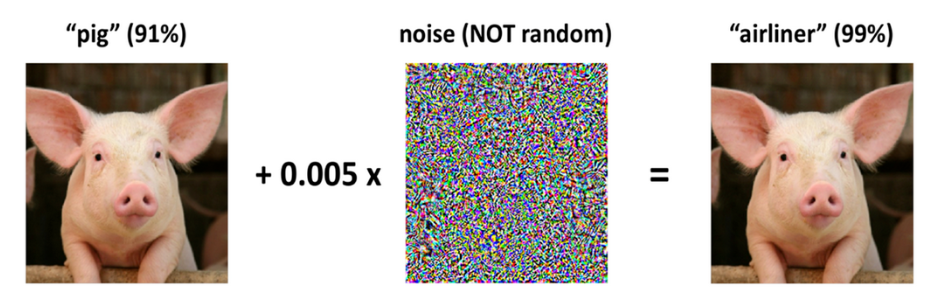
\includegraphics[width=\columnwidth]{01-images/01-titleimage.png}
        \caption{Dieses Bild soll noch ersetzt werden}
        \label{01-titleimage}
    \end{figure}
    
    \vfill

    \large{
    \begin{tabular}{@{}p{7cm}l}
        Studenten                  &    Si Ben Tran\\
                                   &    Gabriel Torres Gamez\\[2ex]
        
        Fachbetreuer               &    Daniel Perruchoud\\
                                   &    Stephan Heule\\[2ex]
                                   
        Auftraggeber               &    i4Ds\\
        Projektnummer              &    24FS\_I4DS\\[4ex]
        
        \multicolumn{2}{@{}l}{Fachhochschule Nordwestschweiz, Hochschule für Technik} %Hochschule für Informatik
    \end{tabular}
    }
    
    % Logo
    \begin{tikzpicture}[remember picture,overlay,every node/.style={anchor=north east}]
      \node at (current page.north east) [xshift=-1cm, yshift=-0.4cm] {
\includegraphics[width=4cm]{01-images/02-logo.png}};
    \end{tikzpicture}
    
    \begin{tikzpicture}[remember picture,overlay,every node/.style={anchor=north west}]
      \node at (current page.north west) [xshift=1cm, yshift=-1.2cm] {
\includegraphics[width=9cm]{01-images/03-fhnwlogo.pdf}};
    \end{tikzpicture}
    
    \clearpage
    
\end{titlepage}

\section*{Abstract} 

abstract

\todo{eigenleistung uap alg}

\clearpage
\section*{Vorwort und Dank}

danke

    

\tableofcontents{}

% Einleitung
\section{Einleitung}
Die Entwicklung von Deep Learning Modellen führte in den letzten Jahren zu signifikanten Fortschritten in der Bildklassifikation. Jedoch zeigen Studien \cite{szegedy_intriguing_2014}\cite{goodfellow_explaining_2015}, dass diese Modelle anfällig für sogenannte Adversarial Attacks sein können. Eine besondere Form solcher Angriffe sind Universal Adversarial Perturbations (\acrshort{uap}s) \cite{moosavi-dezfooli_universal_2017}, gezielt erzeugtes Rauschen, das auf verschiedene Eingabebilder addiert werden kann, um Fehlklassifikationen zu verursachen. Die vorliegende Thesis untersucht die Auswirkungen von \acrshort{uap}s auf Deep Learning Modelle im Kontext der binären Klassifikation medizinischer Bilder sowie Methoden zur Erhöhung der Robustheit dieser Modelle.

Das Hauptziel dieser Thesis ist, die Robustheit von Deep Learning Modellen gegenüber \acrshort{uap}s zu untersuchen und zu verbessern. Dabei werden insbesondere die Modelle ResNet, DenseNet und EfficientNet analysiert. Ein weiteres Ziel ist die Entwicklung und Implementierung eines anwendungsspezifischen Algorithmus zur Generierung von \acrshort{uap}s sowie die Evaluierung von Adversarial Training als Verteidigungsmechanismus.

Zur Erreichung dieser Ziele wird ein mehrstufiger Ansatz verfolgt. Zunächst werden die genannten Modelle auf zwei medizinischen Datensätzen (COVIDx CXR-4 und Brain Tumor) trainiert. Anschliessend wird ein angepasster Algorithmus zur Generierung von \acrshort{uap}s implementiert, der auf die Erhöhung der Falsch-Negativ-Rate abzielt. Die Robustheit der Modelle wird dann durch wiederholtes Adversarial Training verbessert. Für die technische Umsetzung kommen die Deep Learning Frameworks PyTorch und PyTorch-Lightning zum Einsatz, während der Trainingsprozess mit Weights \& Biases überwacht wird.

Die Untersuchungen zeigen, dass \acrshort{uap}s in der Lage sind, die Leistung der Modelle signifikant zu beeinträchtigen, insbesondere hinsichtlich der Recall-Metriken. Obwohl Adversarial Training die Robustheit der Modelle verbessern kann, bleiben diese weiterhin anfällig für neu generierte \acrshort{uap}s. Eine wichtige Erkenntnis ist, dass die \Gls{robustifizierung} in einigen Fällen dazu führt, dass grössere Perturbationen erforderlich sind, um die Modelle zu täuschen, was die Zeitintensität der \acrshort{uap}-Generierung erhöht.

Die vorliegende Thesis ist wie folgt strukturiert: Nach dieser Einleitung werden in Kapitel 2 die theoretischen Grundlagen von Adversarial Attacks und \acrshort{uap}s erläutert. Kapitel 3 beschreibt die verwendeten Datensätze. In Kapitel 4 wird die angewandte Methodik detailliert dargestellt, einschliesslich der Modellarchitekturen, des \acrshort{uap}-Algorithmus und des Adversarial Trainings. Kapitel 5 präsentiert und interpretiert die Ergebnisse der Untersuchungen, während Kapitel 6 diese diskutiert und einen Ausblick auf zukünftige Forschungsrichtungen gibt.

% Grundlagen 
\section{Grundlagen, Stand der Forschung}
\subsection{Adversarial Attacks}

Adversarial Attacks sind ein faszinierendes Phänomen im Bereich des Deep Learning, das in den letzten Jahren zunehmend an Bedeutung gewonnen hat. Diese Angriffe beziehen sich auf gezielte Manipulationen von Eingabedaten, die darauf abzielen, neuronale Netzwerke zu täuschen und falsche Vorhersagen zu erzwingen. Sie werfen wichtige Fragen zur Robustheit und Sicherheit von Deep-Learning-Modellen auf und haben weitreichende Implikationen für deren praktische Anwendungen. 
\todo{Erste Paper mit Perturbationen z.B. Paper von Goodfellow}

\subsubsection{Grundlagen}


\subsubsection{Allgemeine Beispiele für Adversarial Attacks}
\subsubsection{Adversarial Attacks auf Bildklassifikation}

\subsection{Universal Adversarial Attacks auf Bildklassifikation}
\subsubsection{Grundlagen}
\subsubsection{Unser Hauptpaper}
\subsubsection{Bisherige Herausforderungen bei der Verteidigung}

% Daten
\section{Daten}\label{chap:Daten}

In unserer Arbeit konzentrieren wir uns primär auf zwei Datensätze, die jeweils medizinische Bilder von Patienten enthalten, die entweder an COVID-19 erkrankt sind (im COVIDx CXR-4 Datensatz) oder an Gehirntumoren leiden (im Brain Tumor Datensatz). Diese Datensätze weisen die Gemeinsamkeit auf, dass sie medizinische Bildinformationen enthalten. 

\subsection{COVIDx CXR-4} \label{chap:COVIDX-CXR4}
\subsubsection{COVID-19} \label{chap:covid19 allgemein}
COVID-19, verursacht durch das Coronavirus SARS-CoV-2, ist eine hochansteckende Atemwegserkrankung, die erstmals Ende 2019 identifiziert wurde. Die Symptome reichen von milden Anzeichen wie Husten und Fieber bis hin zu schweren Krankheitsverläufen, wie Lungenentzündung und akutem Atemnotsyndrom. Aufgrund der hohen Übertragbarkeit und der potenziell schweren Verläufe hatte die Pandemie weitreichende Auswirkungen auf das globale Gesundheitssystem, die Wirtschaft und das tägliche Leben der Menschen. 

\todo{Quelle}

\subsubsection{Datensatz}
\textbf{COVIDx CXR-4} \cite{wu_covidx_2023} ist ein öffentlicher Datensatz für COVID-19-Diagnostik mit Röntgenbildern, der 84,818 Bilder von 45,342 Patienten enthält. COVIDx CXR-4 ist, nach Kenntnisstand der Autoren, der grösste und vielfältigste öffentlich verfügbare COVID-19-Datensatz für Röntgenbilder und soll die Forschung unterstützen, um Klinikern im Kampf gegen COVID-19 zu helfen.

Patienten, mit einem negativen Befund erhalten das Klassenlabel Null, bei einem positiven Befund das Klassenlabel Eins. Diese Unterscheidung ist wichtig und relevant für unsere binäre Klassifikation. Die Röntgenbilder beschränken sich auf den Brustkorb des jeweiligen Menschen.

\begin{figure}[H]
    \centering
    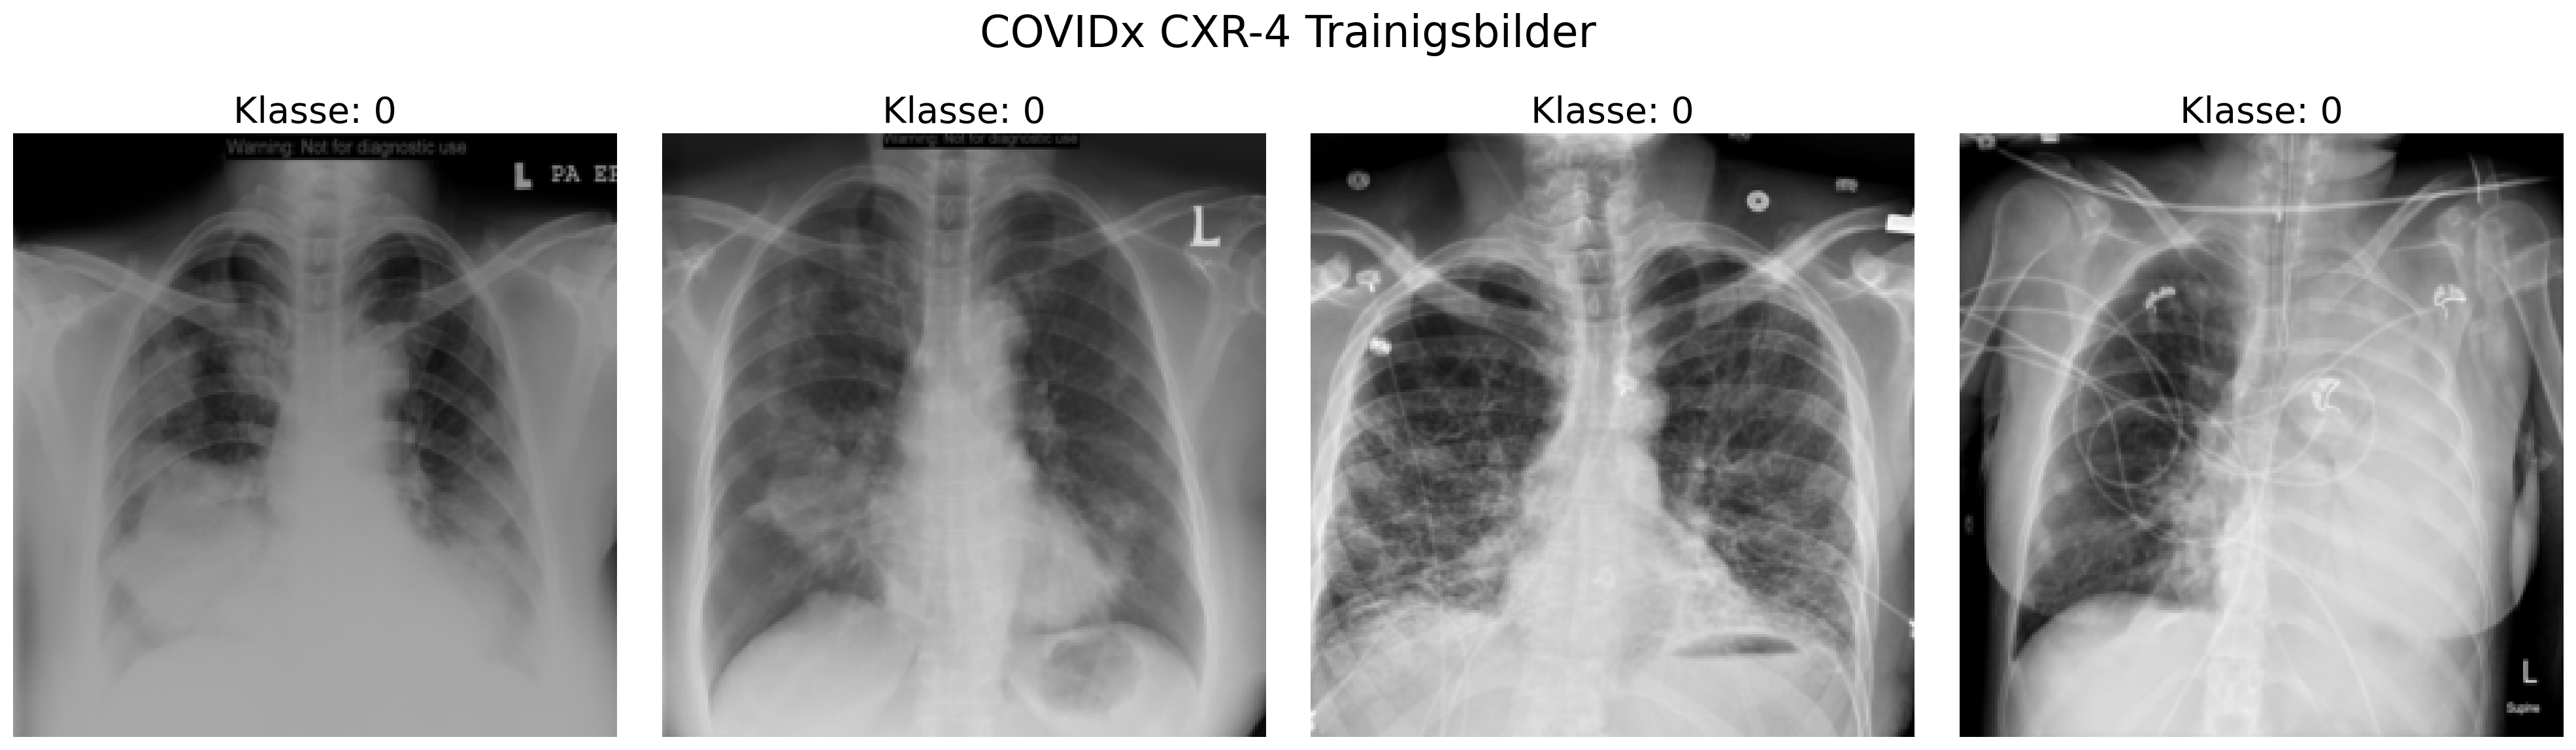
\includegraphics[width=\linewidth, height=4cm]{01-images/03-data/covid19-klasse0.png}
    \caption{Beispiele von negativen Covid Patienten vom COVIDx CXR-4 Datensatz}
    \label{fig:covid19-klasse0}
\end{figure}

\begin{figure}[H]
    \centering
    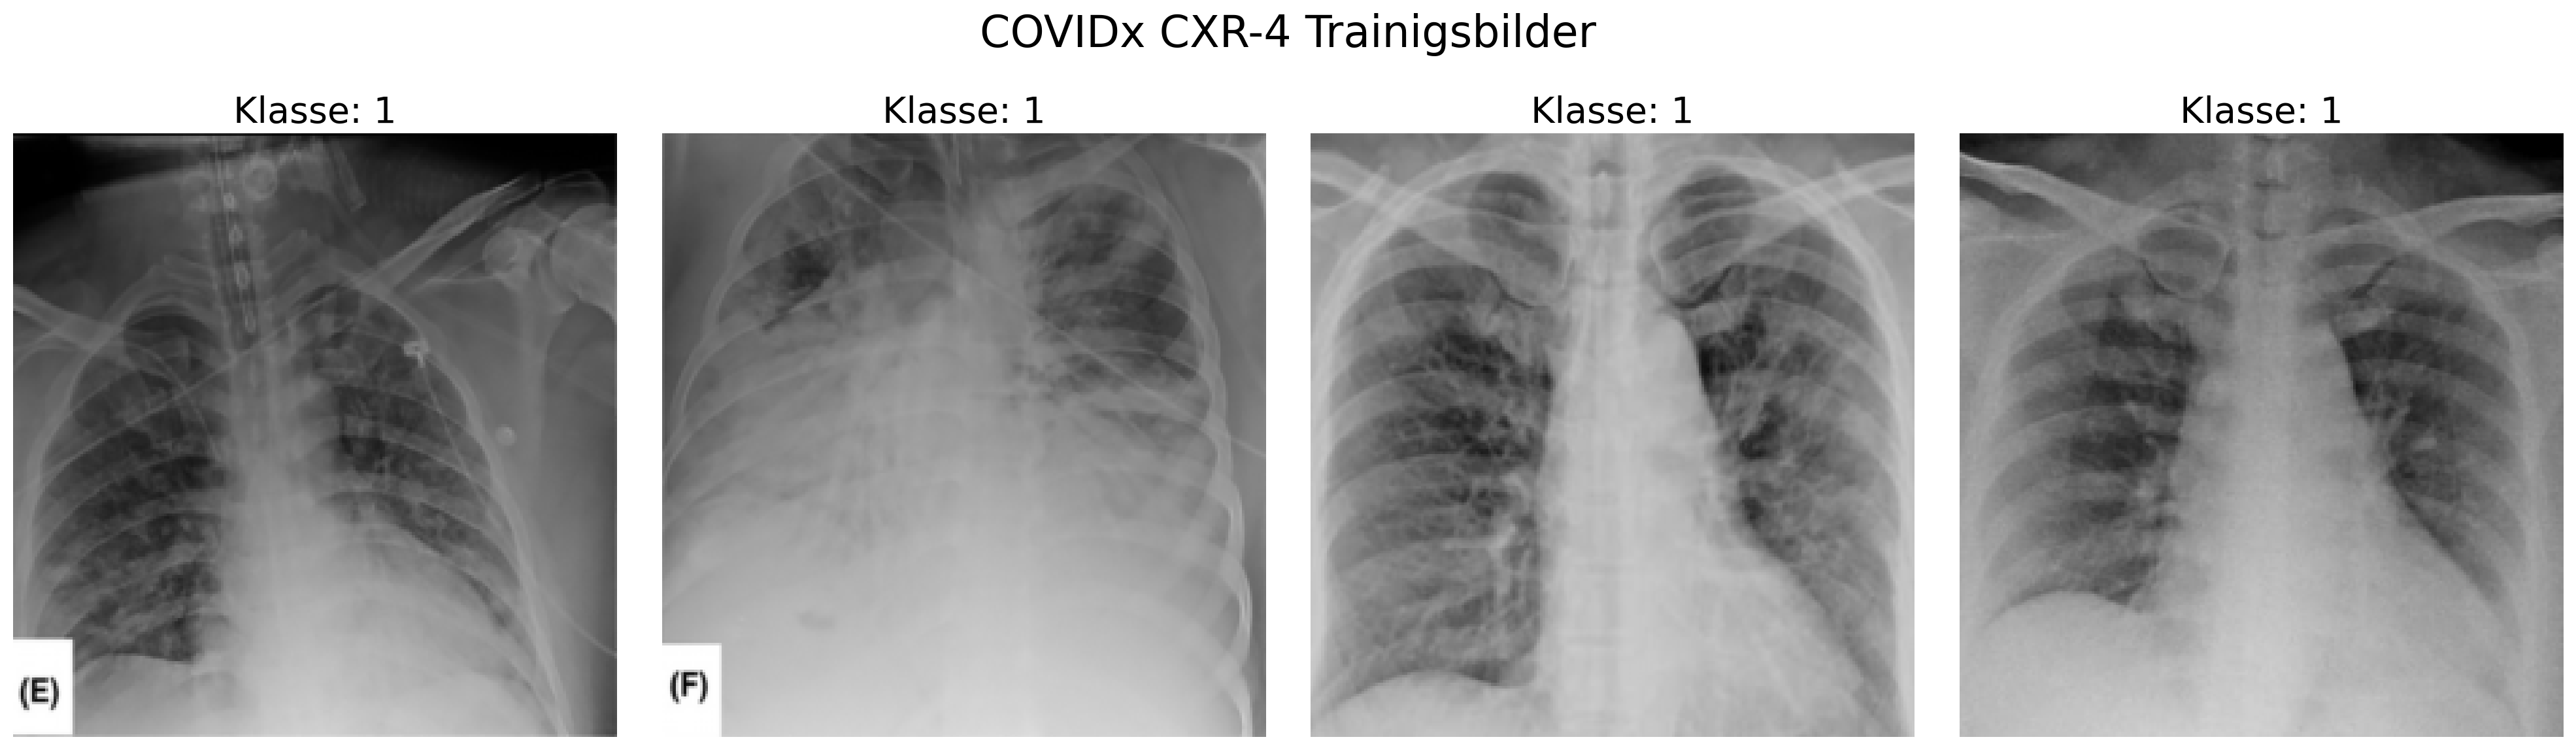
\includegraphics[width=\linewidth, height=4cm]{01-images/03-data/covid19-klasse1.png}
    \caption{Beispiele von positiven Covid Patienten vom COVIDx CXR-4 Datensatz}
    \label{fig:covid19-klasse1}
\end{figure}


\subsubsection{Datenpartitionierung} \label{chap:COVIDX-Partition}

Die Datenpartitionierung ist bereits durch die Struktur vorgegeben. Wir stellen fest, dass die Klassenverteilung von positiven und negativen Labels für die Validierung und den Testdatensets fast gleich verteilt ist, mit einem Verhältnis von 50\% positive sowie 50\% negative Fälle. 

\begin{table}[h]
\centering
\begin{tabular}{@{}cccccc@{}}
\toprule
Partition & \multicolumn{2}{c}{Anzahl Bilder} & \multicolumn{2}{c}{Klassenverteilung} & Positiv-Verhältnis\\ 
\cmidrule(lr){2-3} \cmidrule(lr){4-5} 
          & Absolut & Relativ & Positiv & Negativ & \\ 
\midrule
Train      & 67863 & 0.8001 & 57199 & 10664 & 0.8429 \\
Validation & 8473  & 0.0999 & 4241  & 4232  & 0.5005 \\
Test       & 8482  & 0.1000 & 4241  & 4241  & 0.5000 \\ 
\bottomrule
\end{tabular}
\caption{Klassenverteilung von COVIDX-CXR4}
\label{tab:covidx-klassenverteilung}
\end{table}

\subsubsection{Datenexploration}


In den dargestellten Histogrammen sehen wir die Pixelverteilung der Röntgenbilder von positiven \ref{fig:covid19-klasse1} und negativen \ref{fig:covid19-klasse0} Patienten. Jedes Histogramm repräsentiert die Intensitätsverteilung der Pixelwerte in den jeweiligen Röntgenaufnahmen. Die x-Achse jedes Histogramms zeigt die Grauwertintensität von 0 bis 255, während die y-Achse die Anzahl der Pixel für jede Intensität darstellt. 

\begin{figure}[ht]
    \centering
    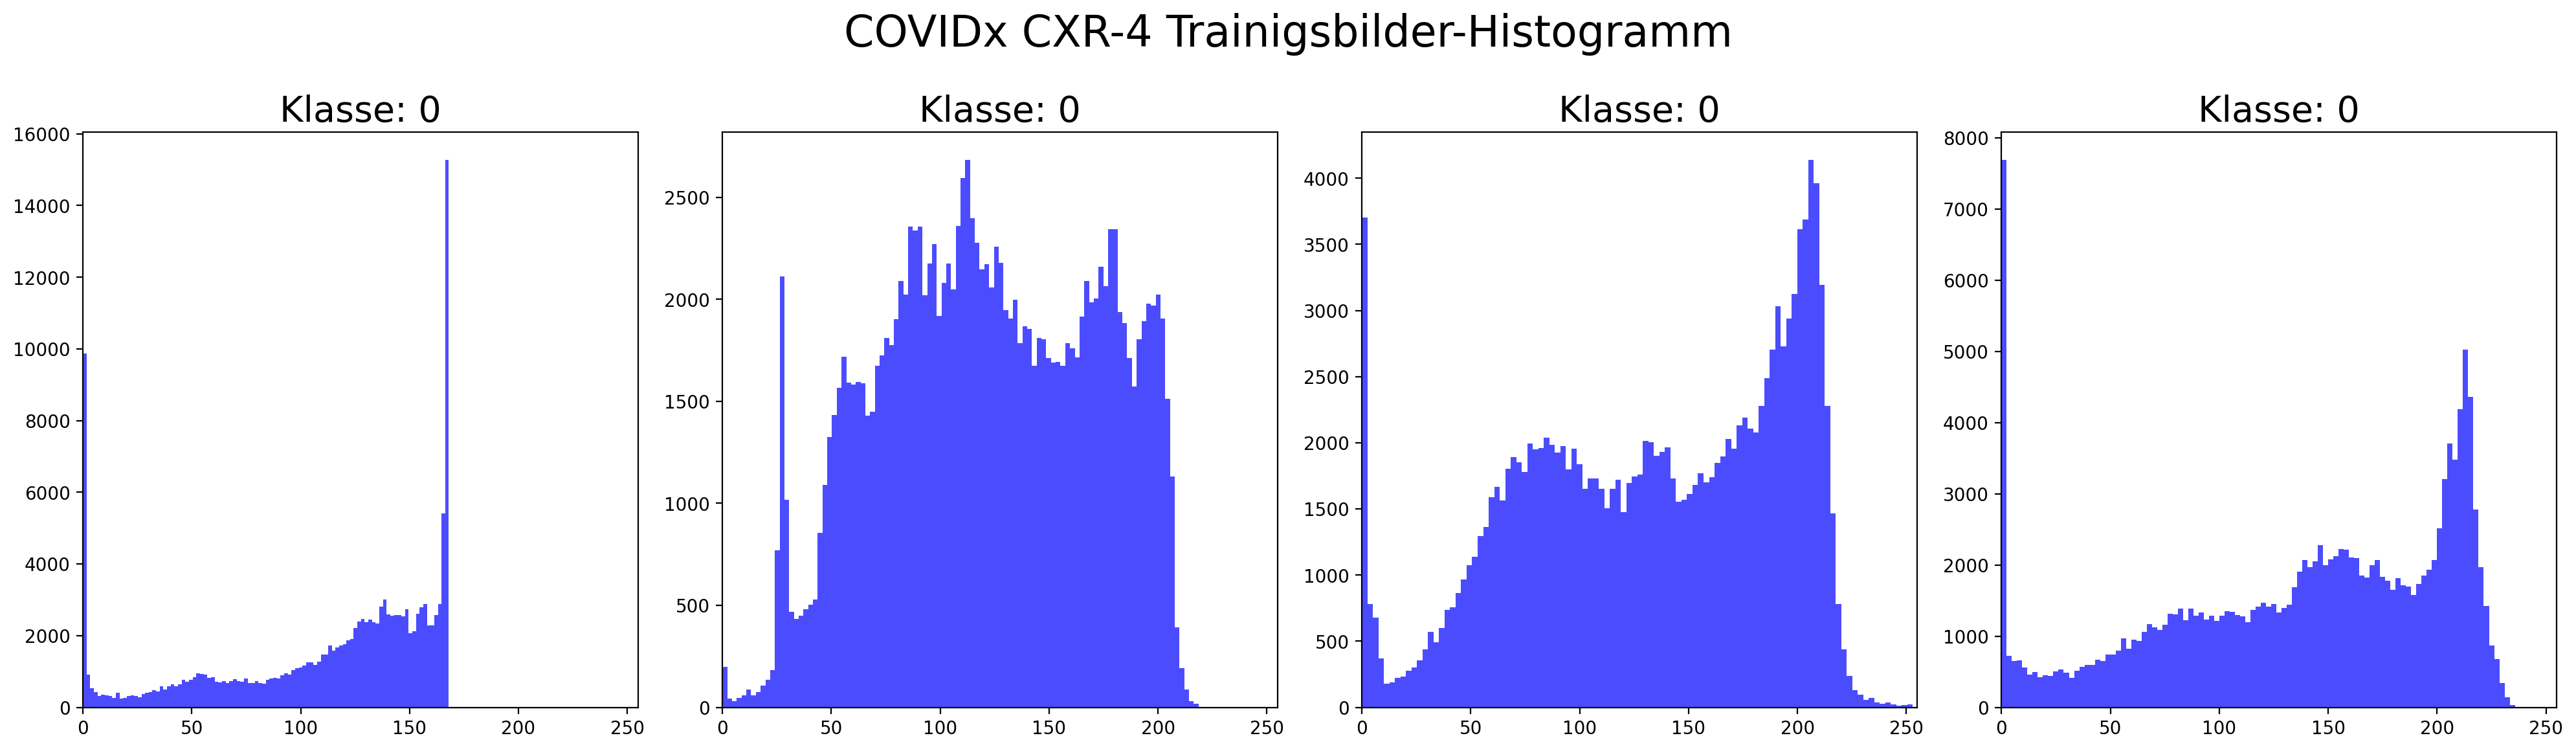
\includegraphics[width=\linewidth, height=4cm]{01-images/03-data/covid19-klasse0-hist.png}
    \caption{Histogramm der Pixelverteilung von Abbildung \ref{fig:covid19-klasse0}}
    \label{fig:covid19-klasse0-hist}
\end{figure}

\begin{figure}[ht]
    \centering
    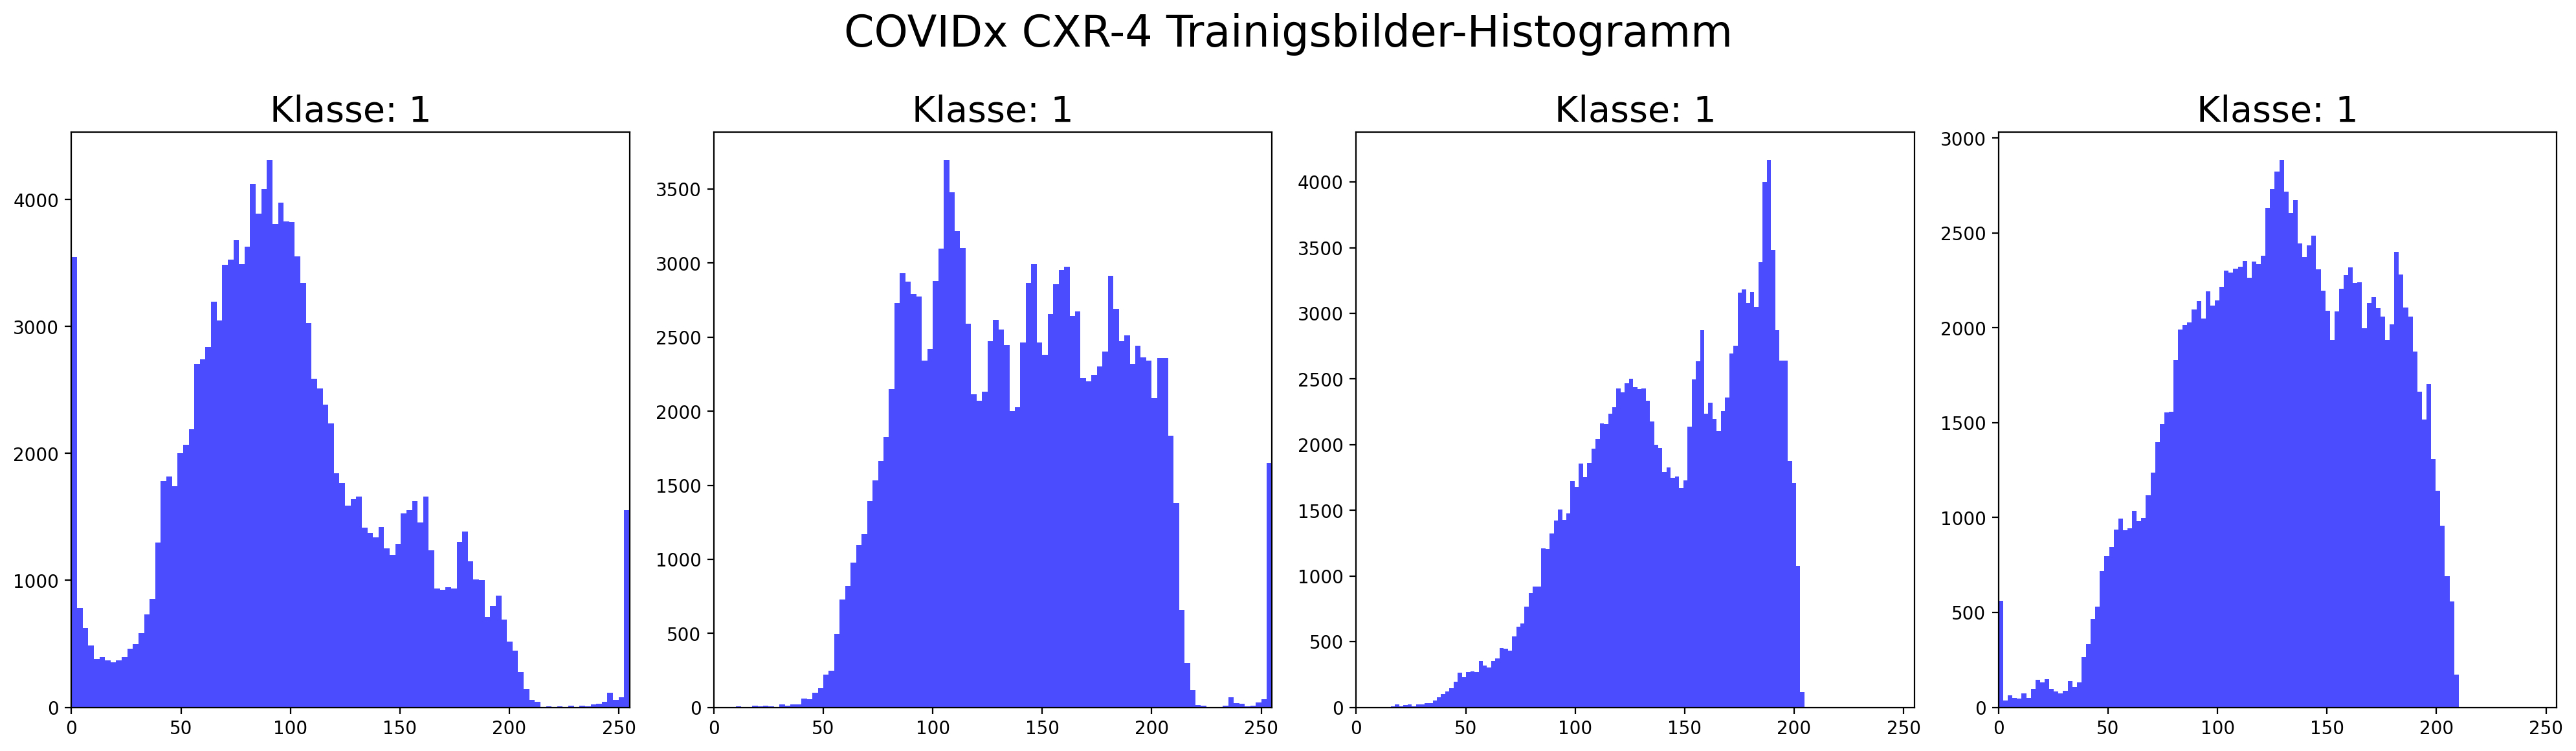
\includegraphics[width=\linewidth, height=4cm]{01-images/03-data/covid19-klasse1-hist.png}
    \caption{Histogramm der Pixelverteilung von Abbildung \ref{fig:covid19-klasse1}}
    \label{fig:covid19-klasse1-hist}
\end{figure}

Die Histogramme der Röntgenbilder variieren stark von Bild zu Bild. Tiefe Pixelwerte repräsentieren vermutlich Weichgewebe, während höhere Pixelwerte harte Knochengewebe darstellen

\subsection{Datenverteilung \& Testperofmance} \label{chap:Datenverteilung-Testperformance-covidx}

Im Verlauf unserer Arbeit stellten wir fest, dass die Performance-Metriken der Testdaten von Covidx nicht den erwarteten Werten entsprechen. Daher führten wir eine umfassende explorative Analyse der Trainings-, Validierungs- und Testdaten durch, um potenzielle Ursachen für diese Diskrepanzen zu identifizieren. In den folgenden Kapiteln \ref{chap:Pixelverteilung-TestProblemEda1-covidx}, \ref{chap:Differenzenbilder-TestProblemEda2-covidx} und \ref{chap:FeatureMaps-TestProblemEda3-covidx} zeigen wir die Resultate der Untersuchungen.

\todo{vorab weg die Resultate schon hier erwaehnen}

\subsubsection{Pixelverteilung} \label{chap:Pixelverteilung-TestProblemEda1-covidx}

Um die Verteilung der Pixelwerte zu analysieren, flachen wir die Bilder zu einem eindimensionalen Vektor ab. Diese Vektoren repräsentieren alle Bilder einer jeweiligen Datenpartition. Die resultierenden Daten visualisieren wir mithilfe von Histogrammen, wie in Abbildung \ref{fig:hist-datapartition-covid} dargestellt.

\begin{figure}[ht]
    \centering
    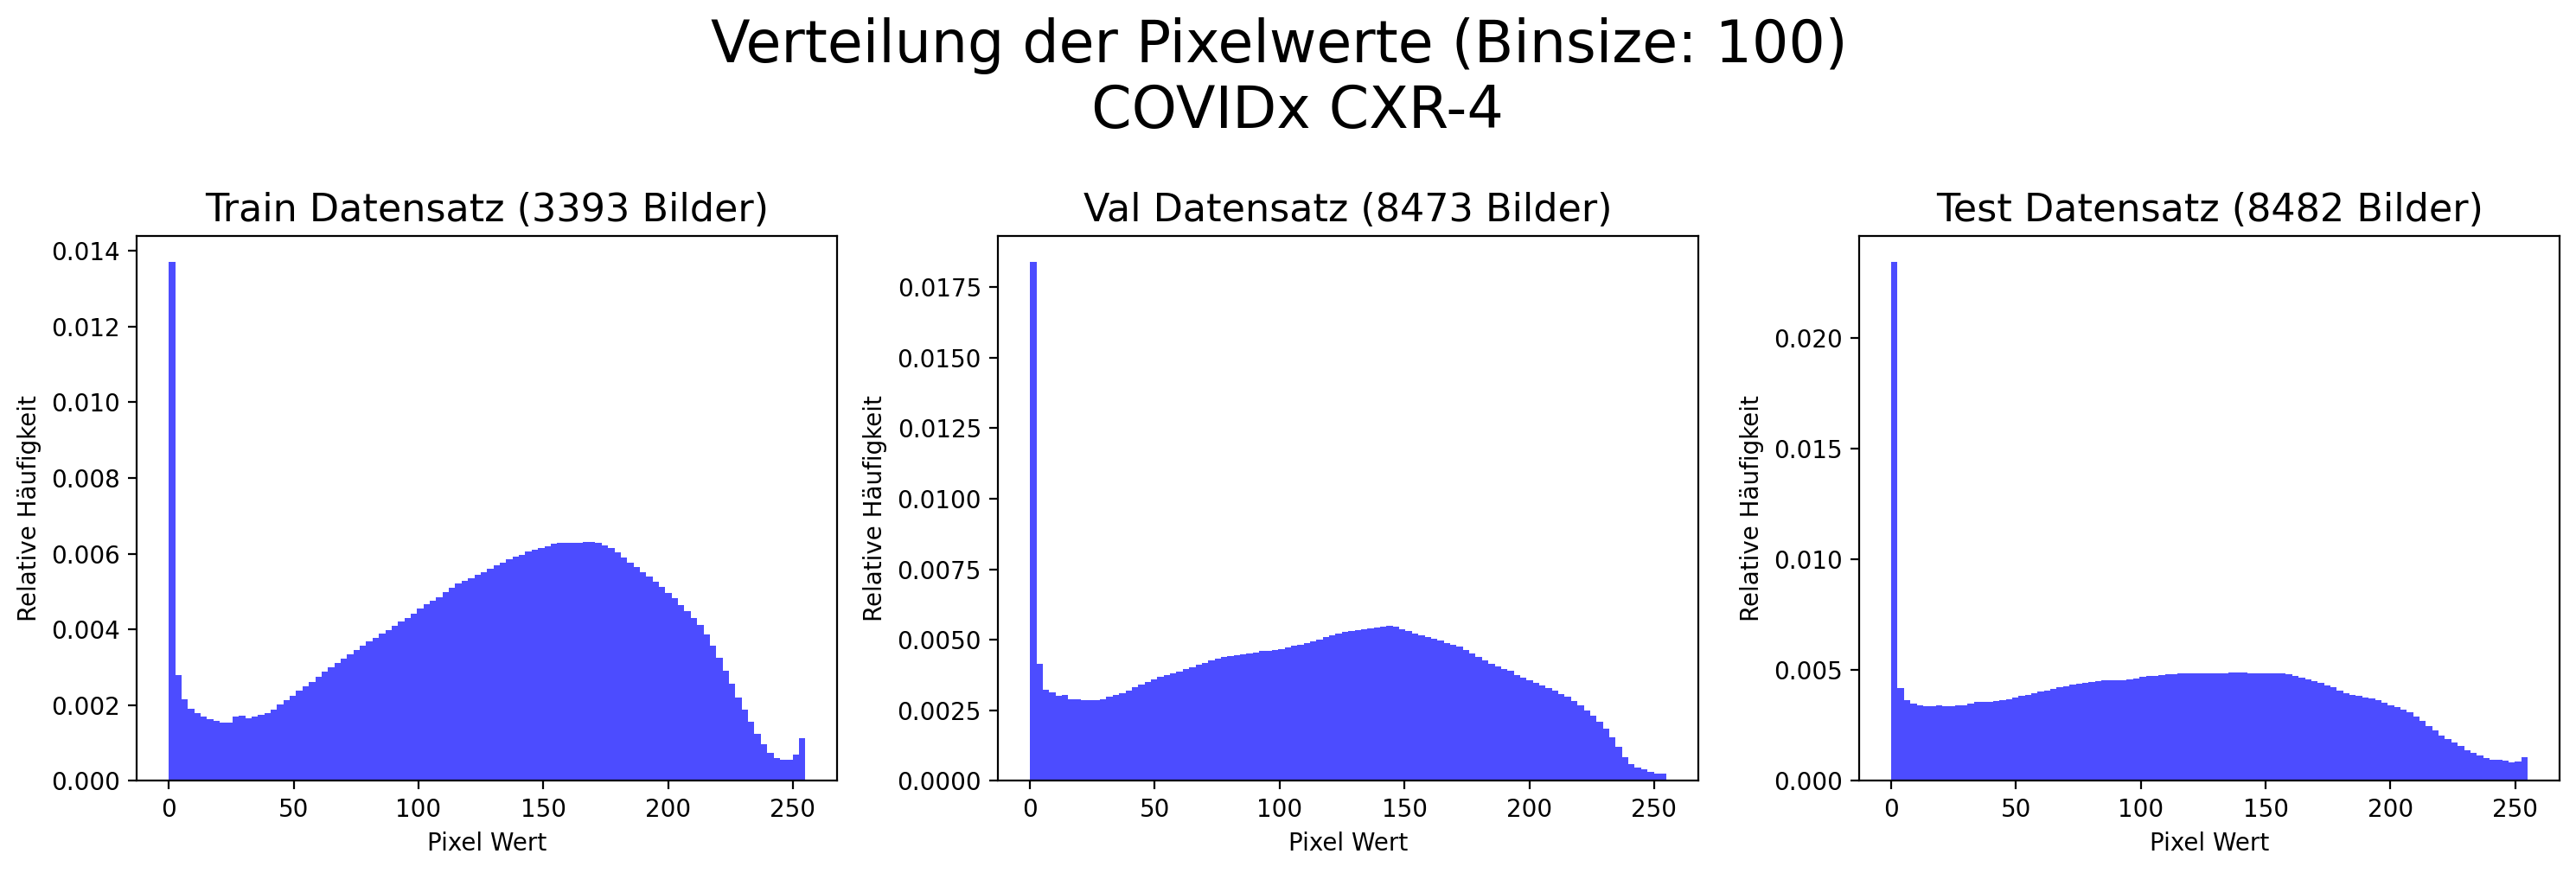
\includegraphics[width=\linewidth, height=5cm]{01-images/03-data/covid-Pixelverteilung-Partitionen.png}
    \caption{Histogramme der Pixelverteilung von Covid in jeder Datenpartition}
    \label{fig:hist-datapartition-covid}
\end{figure}

Die Histogramme verdeutlichen, dass Pixelwerte nahe null, welche schwarzen Pixeln entsprechen, häufig auftreten, was bei Röntgenaufnahmen üblich ist. Besonders auffällig ist der Gipfel, der seinen Höhepunkt bei einem Pixelwert von etwa 180 erreicht. Dieser Gipfel ist auch im Validierungsdatensatz vorhanden, allerdings weniger ausgeprägt und abgeflacht. Im Testdatensatz ist dieser Gipfel nahezu nicht vorhanden. Stattdessen ist am Ende der Verteilung ein leichter Anstieg zu beobachten, der auf die Präsenz von weissen Pixelwerten hinweist. Die Verteilung der Pixelwerte in den Trainings- und Validierungsdaten weisen ein ähnliches Muster auf, jedoch mit unterschiedlichen Intensitäten. Dies könnte auf eine Variation in der Bildaufnahme  zwischen den Partitionen deuten. Der deutliche Unterschied im Testdatensatz, insbesondere das fast völlige Fehlen des typischen Gipfels, könnte auf eine unterschiedliche Charakteristik der Bilder oder eine andere Verteilung in dieser Partition hindeuten. Es lässt sich nicht definitiv ausschliessen oder bestätigen, dass die Testpartitionen einer anderen Verteilung folgen. Dies könnte auf verschiedene Faktoren wie Belichtungszeiten, Sensoreinstellungen oder sogar auf die Art und Weise der Datensammlung, beispielsweise durch unterschiedliche Maschinen zurückzuführen sein.

\subsubsection{Differenzbilder} \label{chap:Differenzenbilder-TestProblemEda2-covidx}

Differenzbilder werden verwendet, um den durchschnittlichen Pixelwert innerhalb jeder Datenpartition in einer festgelegten Dimension von 224 x 224 Pixeln zu berechnen. Diese spezifische Dimension wurde aufgrund der Anforderungen des Preprocessing-Schrittes in unserer Analyse gewählt. Durch die Berechnung des Mittelwerts über alle Bilder einer Partition können diese Bilder dann als Heatmaps visualisiert werden. Ziel dieser Visualisierungsmethode ist es, die Unterschiede zwischen den Partitionen auf eine visuell zugängliche Weise darzustellen und dadurch potenzielle Auffälligkeiten oder Muster zu identifizieren.

\begin{figure}[ht]
    \centering
    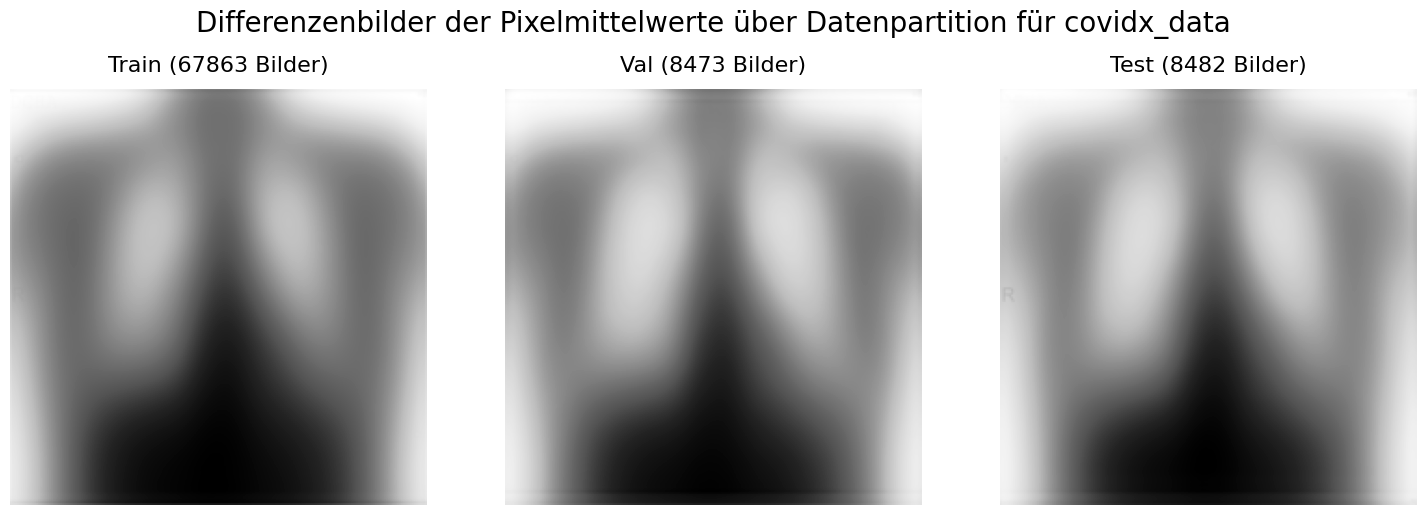
\includegraphics[width=\linewidth, height=5cm]{01-images/03-data/covid-Differenzenbilder-Partition.png}
    \caption{Differenzbilder von Covid in jeder Datenpartition}
    \label{fig:differenzenbilder-datapartition-covid}
\end{figure}

In der Analyse der Differenzbilder der Pixelmittelwerte über die verschiedenen Datenpartitionen für den Covid Datensatz zeigt sich, dass Unterschiede zwischen Trainings,- Validierung,- Testpartition vorhanden sind. Dies ist jedoch nicht verwunderlich, da die Bilder von unterschiedlichen Personen stammen und der Datensatz eine Sammlung von Covid Bilder ist. Die anatomischen Strukturen, wie die Rippenknochen, sind über alle Partitionen hinweg deutlich zu erkennen. 

\subsubsection{Feature Maps \& PCA} \label{chap:FeatureMaps-TestProblemEda3-covidx}

Im Rahmen unserer Analyse nutzen wir ein ResNet50-Modell, das zum einen durch PyTorch vorab trainiert und zum anderen speziell auf unseren Datensatz angepasst wurde. Besonderes Augenmerk liegt auf der Featureextraktion aus dem vorletzten Layer des Modells, direkt vor dem Klassifikationslayer. Die in diesem Schritt gewonnenen Vektoren, auch als Feature Maps bekannt, durchlaufen einer PCA Dimensionsreduktion. Ziel dieser Reduktion ist es, die Dimensionalität der Daten auf zwei Dimensionen zu reduzieren, um eine Visualisierung der verschiedenen Datenpartitionen zu ermöglichen. Die Interpretation erweist sich als sehr komplex und die Ergebenisse sind nur schwer zu interpretieren. 


\newpage
\subsection{Brain Tumor Datenset} \label{chap:Brain-Tumor}

\subsubsection{Hirntumor} \label{chap:Hirntumor}
Hirntumoren sind abnormale Wucherungen von Zellen im Gehirn, die entweder gutartig oder bösartig sein können. Diese Tumoren können sowohl im Gehirn selbst entstehen als auch als Metastasen von anderen Krebsarten in den Kopf wandern. Die Symptome variieren je nach Tumorart, -grösse und -lokalisation und können Kopfschmerzen, Übelkeit, Sehstörungen, Krampfanfälle und kognitive Beeinträchtigungen umfassen. Aufgrund ihrer Komplexität und der sensiblen Lage im zentralen Nervensystem stellen Hirntumoren eine erhebliche Herausforderung für die medizinische Diagnostik und Behandlung dar und haben oft weitreichende Auswirkungen auf die Lebensqualität der Betroffenen. 

\todo{Quelle}

\subsubsection{Datensatz}
Der \textbf{Brain Tumor Classification (MRI)-Datensatz} \cite{bhuvaji_brain_2020} umfasst 3.260 bereinigte und augmentierte, T1-gewichtete, kontrastverstärkte MRI-Bilder zur Identifikation und Klassifikation von Hirntumoren. 

Die MRI-Bilder in der Abbildung zeigen Beispiele von Gehirnscans, die zur Klassifikation von Hirntumoren verwendet werden. Positive Fälle werden mit der Klasse 1 und negative Fälle mit der Klasse 0 gekennzeichnet. Eine genaue Beschreibung der Klassenzusammenfassung findet sich in Kapitel \ref{chap:Brain-Tumor-Partition}. In den Beispielabbildungen \ref{fig:brain-klasse0} und \ref{fig:brain-klasse1} erkennen wir, dass im Datensatz Saggital-, Frontal- und Transversalebenen des Kopfes enthalten sind.

\begin{figure}[ht]
    \centering
    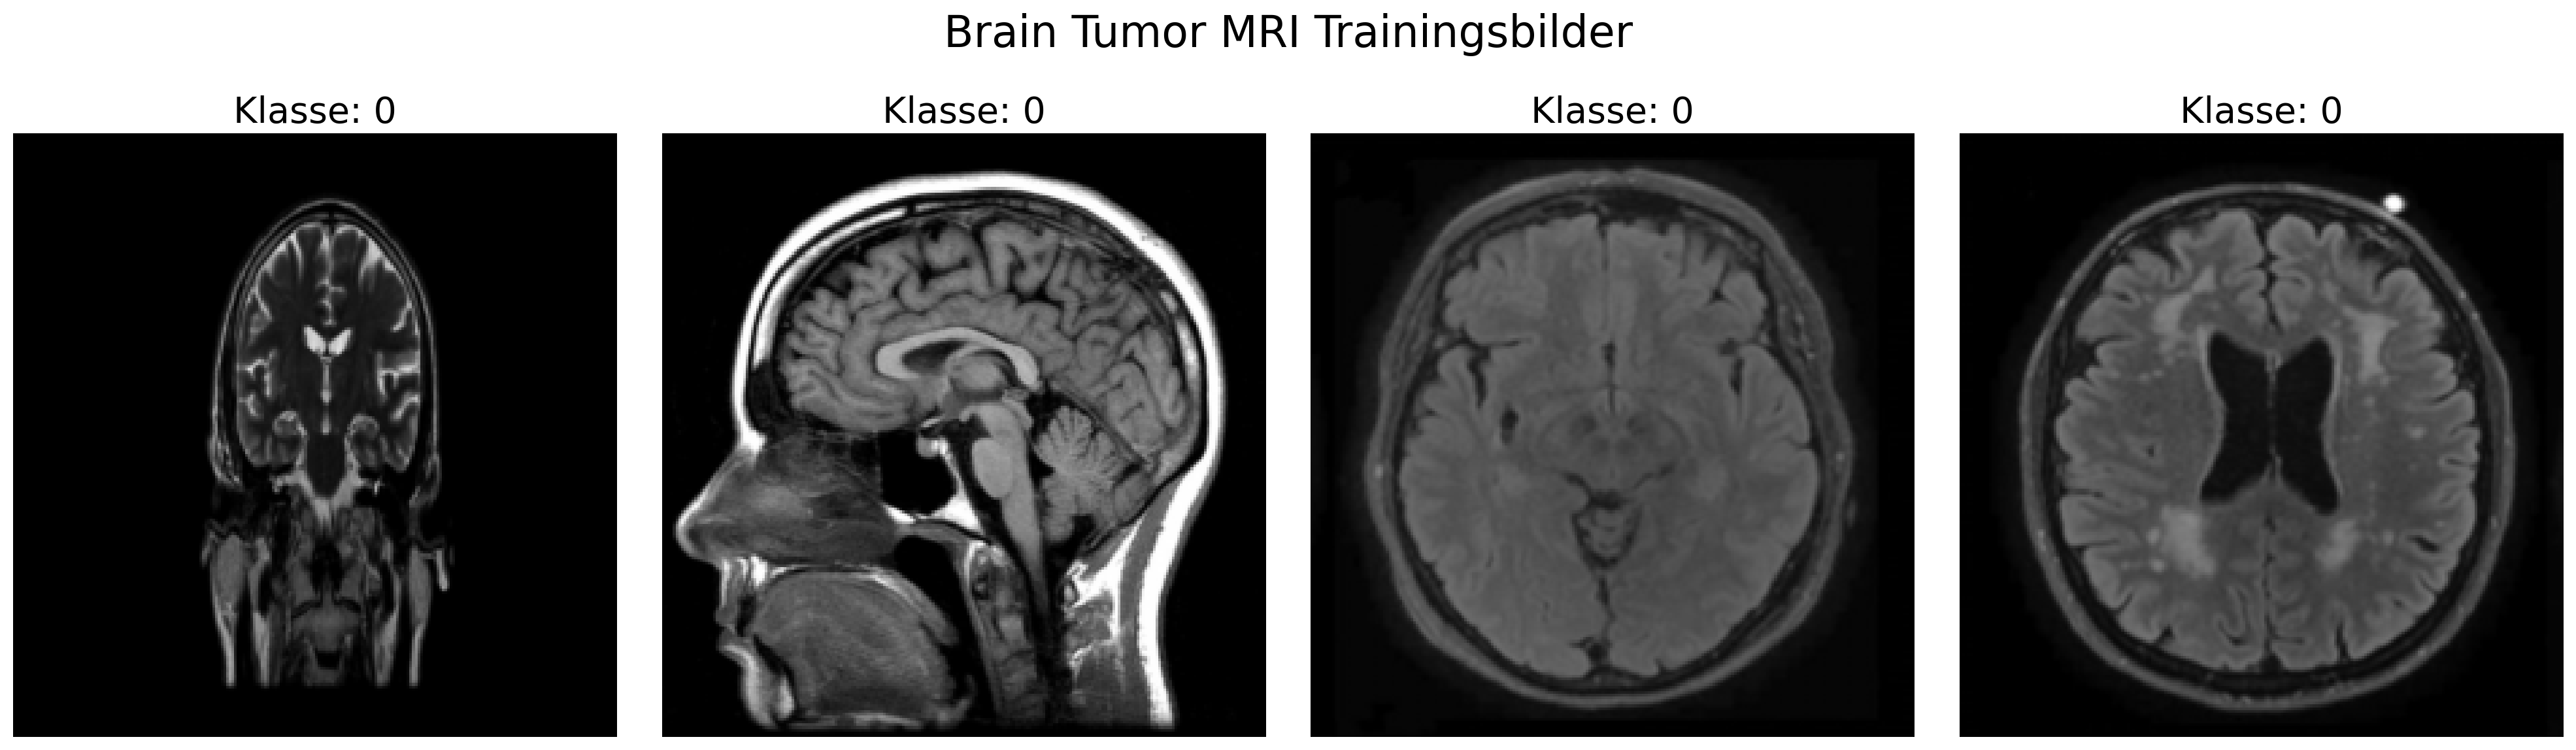
\includegraphics[width=\linewidth, height=4cm]{01-images/03-data/brain-klasse0.png}
    \caption{Beispiele von negativen Hirntumor Patienten vom Brain Tumor Datensatz}
    \label{fig:brain-klasse0}
\end{figure}

\begin{figure}[ht]
    \centering
    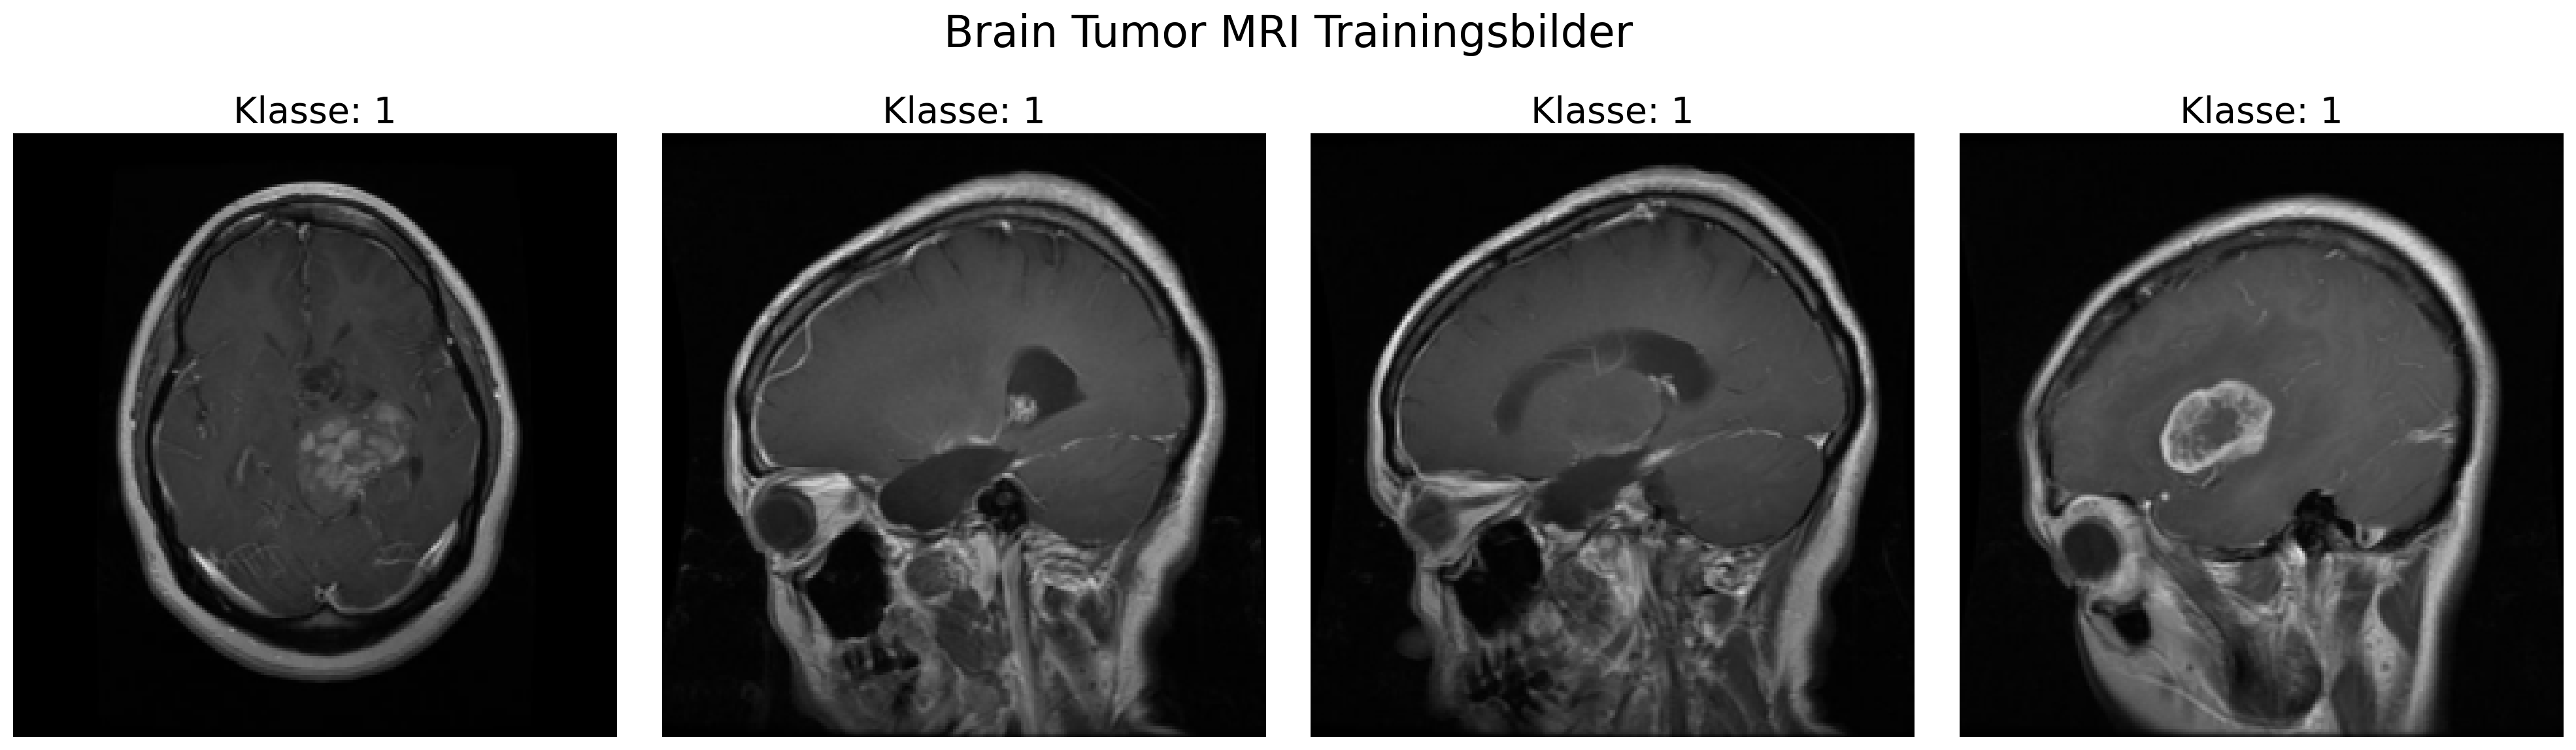
\includegraphics[width=\linewidth, height=4cm]{01-images/03-data/brain-klasse1.png}
    \caption{Beispiele von positiven Hirntumor Patienten vom Brain Tumor Datensatz}
    \label{fig:brain-klasse1}
\end{figure}

\newpage

\subsubsection{Hirntumorarten im Datensatz}
Im Datensatz für Hirntumoren gibt es vier Klassen. Drei davon sind positive Fälle, in denen Hirntumoren vorhanden sind. Eine Klasse ist negativ und beinhaltet keine Hirntumoren. Die drei positiven Klassen sind Gliome, Maligne Tumoren und Pituary.


\paragraph{Gliome}
Gliome sind eine Gruppe von Hirntumoren, die im Glia-Gewebe (Gewebe im Nervensystem) entstehen. Sie sind die häufigsten primären Hirntumoren bei Erwachsenen. Gliome werden nach ihren Ursprungszellen in Astrozytome, Oligodendrogliome und Ependymome unterteilt. Die Symptome variieren je nach Lage und Grösse des Tumors und können Kopfschmerzen, Anfälle und neurologische Defizite umfassen. Die Behandlung erfolgt in der Regel durch eine Kombination von Operation, Strahlentherapie und Chemotherapie.

\paragraph{Malignent}
Maligne Tumoren sind bösartige Wucherungen, die unkontrolliert wachsen und in umliegendes Gewebe eindringen können. Sie haben die Fähigkeit, Metastasen zu bilden, was bedeutet, dass sie sich auf andere Teile des Körpers ausbreiten können. Die Behandlung von malignen Tumoren umfasst in der Regel eine Kombination aus Operation, Strahlentherapie und Chemotherapie. Die Prognose hängt von der Art, dem Stadium und der Lage des Tumors ab.

\paragraph{Pituary}
Hypophysenadenome sind gutartige Tumoren der Hypophyse, einer kleinen Drüse im Gehirn, die wichtige Hormone produziert. Obwohl sie meist nicht bösartig sind, können sie aufgrund ihrer Lage und Hormonproduktion erhebliche gesundheitliche Probleme verursachen. Symptome können Kopfschmerzen, Sehstörungen und hormonelle Ungleichgewichte umfassen. Die Behandlung umfasst in der Regel eine Operation und, in einigen Fällen, medikamentöse Therapie oder Strahlentherapie.

\subsubsection{Datenpartitionierung} \label{chap:Brain-Tumor-Partition}

Der Datensatz enthält ursprünglich nur ein Trainings- und ein Testset. Da uns ein Validierungsset fehlt, erstellen wir dieses aus dem gegebenen Trainingsset. Der Datensatz umfasst vier Klassen, drei davon sind Tumorklassen und eine Klasse ist kein Tumor. Die Verteilung der Klassen ist in der Tabelle \ref{tab:mri-orginale-klassenverteilung} zu sehen. Ersichtlich ist, dass in dem Datensatz positive Tumorklassen deutlich mehr vertreten sind als keine Tumore. Da wir uns für unsere These auf die binäre Klassifikation stützen, fassen wir die drei Hirntumoren Klassen Pituitary, Glioma, Meningioma zu einem positiven Gehirn Tumor Klasse und kein Tumor als negative Klasse und erhalten somit die Tabelle \ref{tab:mri-binaere-klassenverteilung}.

\begin{table}[ht]
\centering
\begin{tabular}{@{}ccccc@{}}
\toprule
 Partition & \multicolumn{4}{c}{Klassenverteilung}        \\ 
\cmidrule(l){2-5}
           & Pituitary & Glioma & Meningioma & kein Tumor \\ 
\midrule 
Train      & 662 & 661 & 658 & 317 \\
Validation & 165 & 165 & 164 & 78  \\
Test       & 74  & 100 & 115 & 105 \\ 
\bottomrule
\end{tabular}
\caption{Ursprüngliche Klassenaufteilung von Hirntumoren}
\label{tab:mri-orginale-klassenverteilung}
\end{table}

Die Verteilungsverhältnisse waren ursprünglich 70.4\% Trainings- und 29.6\% Testbilder. Da ein analoger Datensatz, wie beim COVIDx, einfacher zu handhaben ist, haben wir den ursprünglichen Testdatensatz weiter unterteilt, und zwar in 17.5\% Validierungs- und 12.1\% Testdaten. Bevor wir die positiven Klassen zusammengefasst haben, herrschte eine Klassenimbalance, die wir bei der Partitionierung in Train-, Validierung, und Testset mitberücksichtigt haben. Die Tabelle \ref{tab:mri-binaere-klassenverteilung} zeigt die Anzahl an Bilder in absolut, relativ und die Klassenverteilung von positive, negative Tumorbilder für jede Datenpartition auf.

\begin{table}[ht]
\centering
\begin{tabular}{@{}cccccc@{}}
\toprule
Partition & \multicolumn{2}{c}{Anzahl Bilder} & \multicolumn{2}{c}{Klassenverteilung} & Positiv-Verhältnis\\ 
\cmidrule(lr){2-3} \cmidrule(lr){4-5} 
           & Absolut & Relativ & Positiv & Negativ \\ 
\midrule
Train      & 2298 & 0.704 & 1981 & 317 & 0.862 \\
Validation & 572  & 0.175 & 494  & 78  & 0.864 \\
Test       & 394  & 0.121 & 289  & 105 & 0.736 \\ 
\bottomrule
\end{tabular}
\caption{Binäre Klassenverteilung von Hirntumoren}
\label{tab:mri-binaere-klassenverteilung}
\end{table}

\subsubsection{Datenexploration}

Die Histogramme der Hirntumor-Klassifikation sehen im Vergleich zum COVIDx CXR-4-Datensatz deutlich unterschiedlich aus. So ist klar in den Beispielen ersichtlich, dass die Intensität von niedrigeren Pixelwerten sehr hoch.

\begin{figure}[ht]
    \centering
    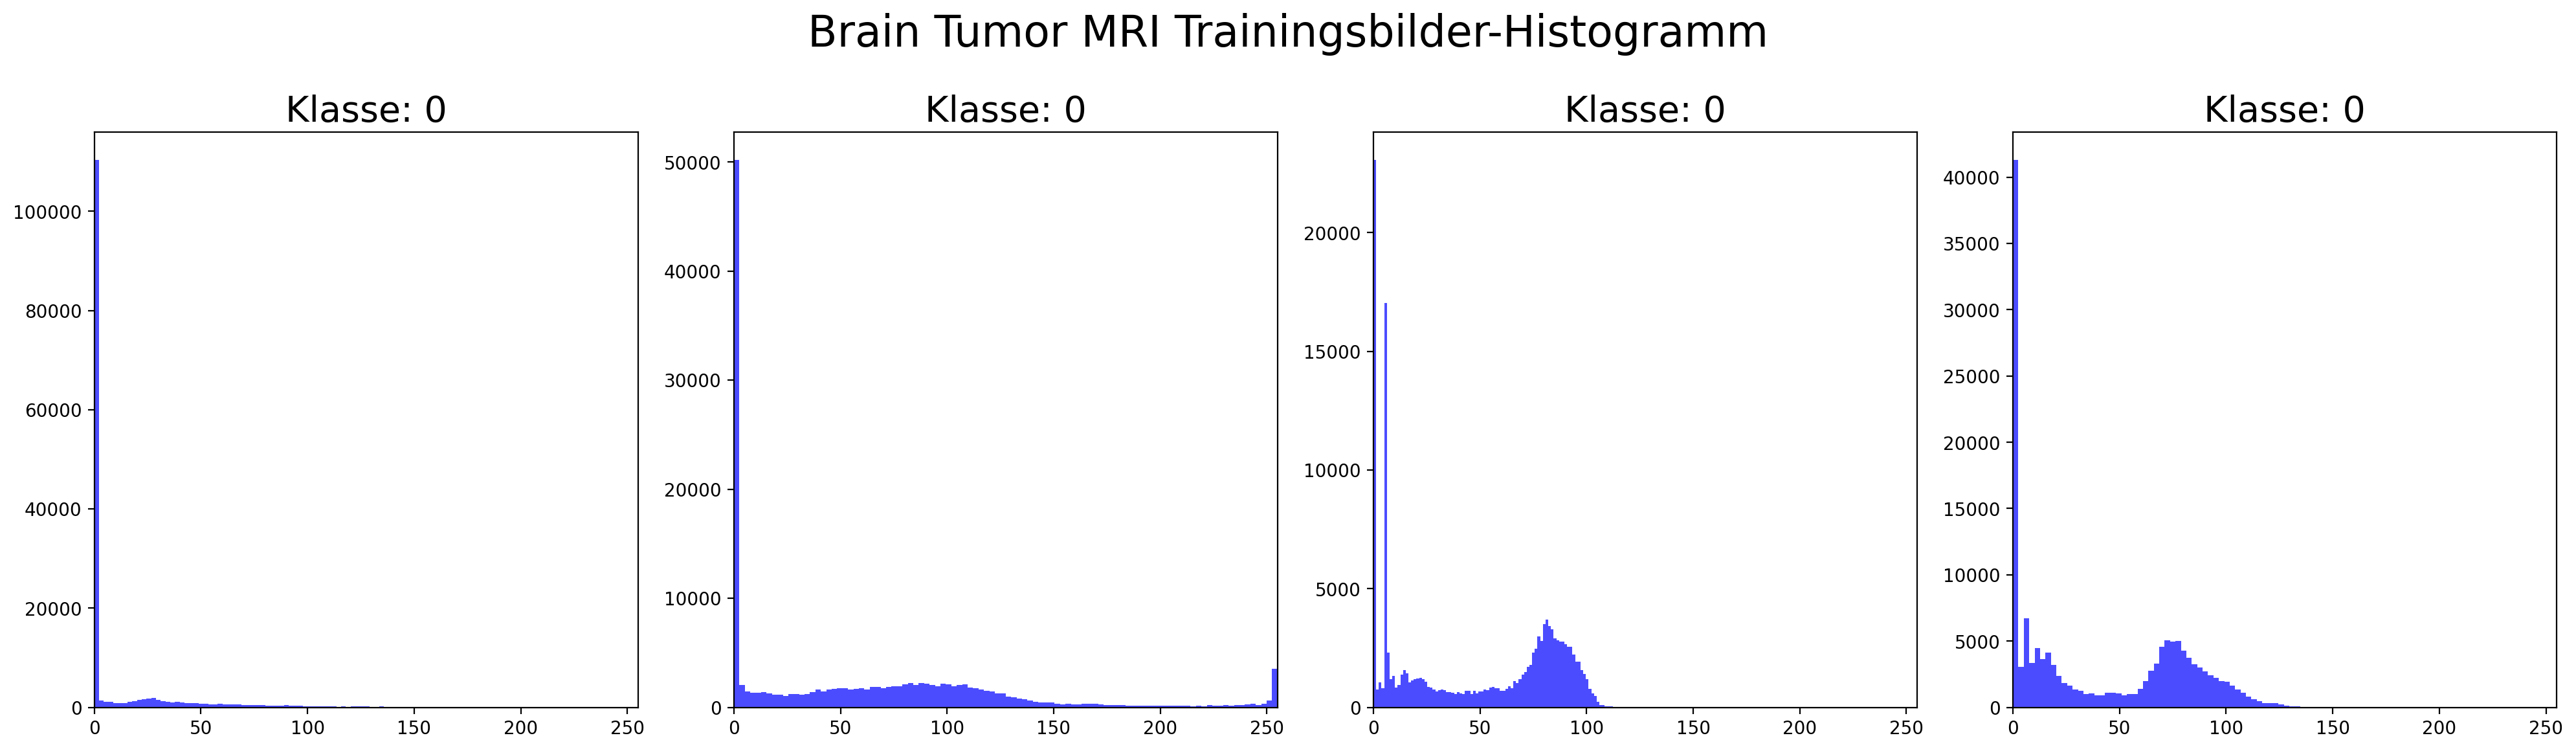
\includegraphics[width=\linewidth, height=4cm]{01-images/03-data/brain-klasse0-hist.png}
    \caption{Histogramm der Pixelverteilung von Abbildung \ref{fig:brain-klasse0}}
    \label{fig:brain-klasse0-hist}
\end{figure}

\begin{figure}[ht]
    \centering
    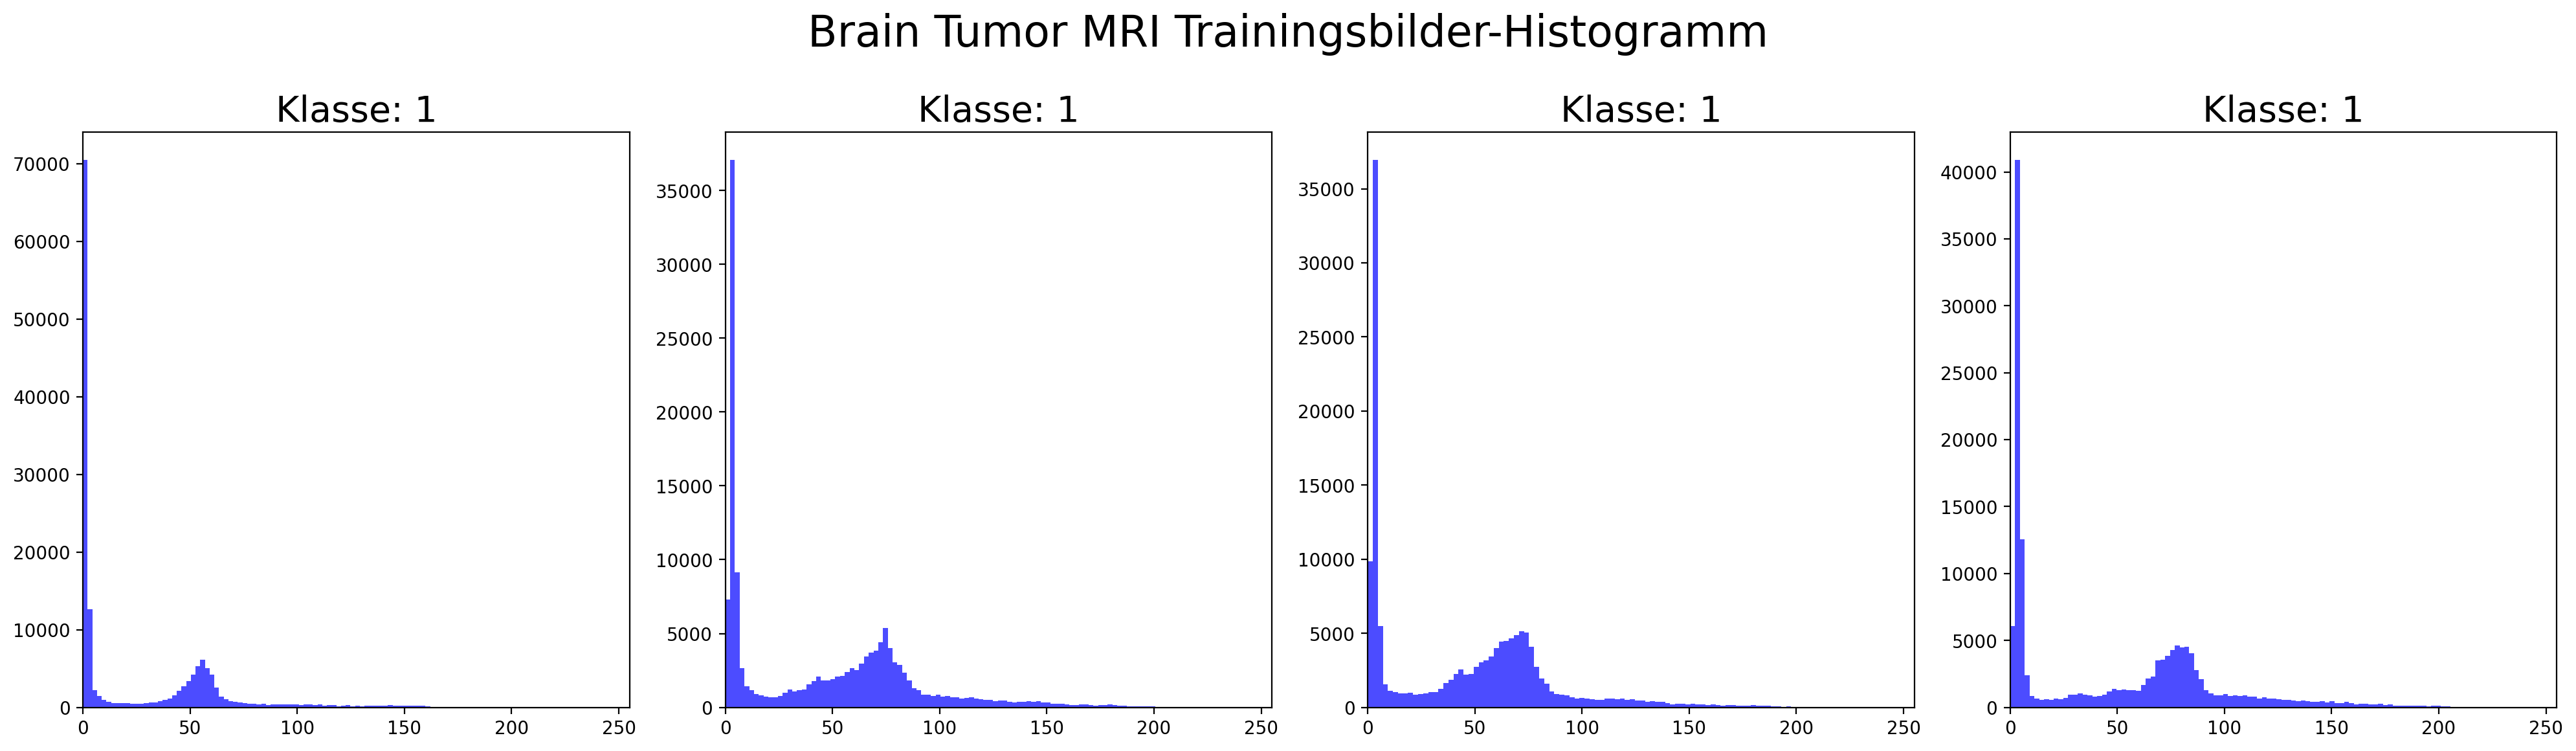
\includegraphics[width=\linewidth, height=4cm]{01-images/03-data/brain-klasse1-hist.png}
    \caption{Histogramm der Pixelverteilung von Abbildung \ref{fig:brain-klasse1}}
    \label{fig:brain-klasse1-hist}
\end{figure}

Die niedrigen Pixelwerte in einem Bild deuten darauf hin, dass viele dunkle Bereiche vorhanden sind. Es liegt nahe, dass dies der Hintergrund der MRI-Bilder ist und somit einen Grossteil der Informationen ausmacht, die keine relevanten Details enthalten.



\subsection{Datenverteilung \& Testperofmance} \label{chap:Datenverteilung-Testperformance-mri}

Wie im Kapitel \ref{chap:Datenverteilung-Testperformance-covidx} haben wir das Problem der Performance auf den Testmetriken ebenfalls auf den MRI Datensatz. 

\subsubsection{Pixelverteilung} \label{chap:Pixelverteilung-TestProblemEda1-mri}


Das Vorgehen, analog zu dem im Kapitel \ref{chap:Pixelverteilung-TestProblemEda1-covidx} beschriebenen, nutzen wir für unseren Hirntumor Datenpartitionen. In der Abbildung \ref{fig:hist-datapartition-brain} zeigt die Histogramme der Pixelwerte für jede Datenpartition.

\begin{figure}[ht]
    \centering
    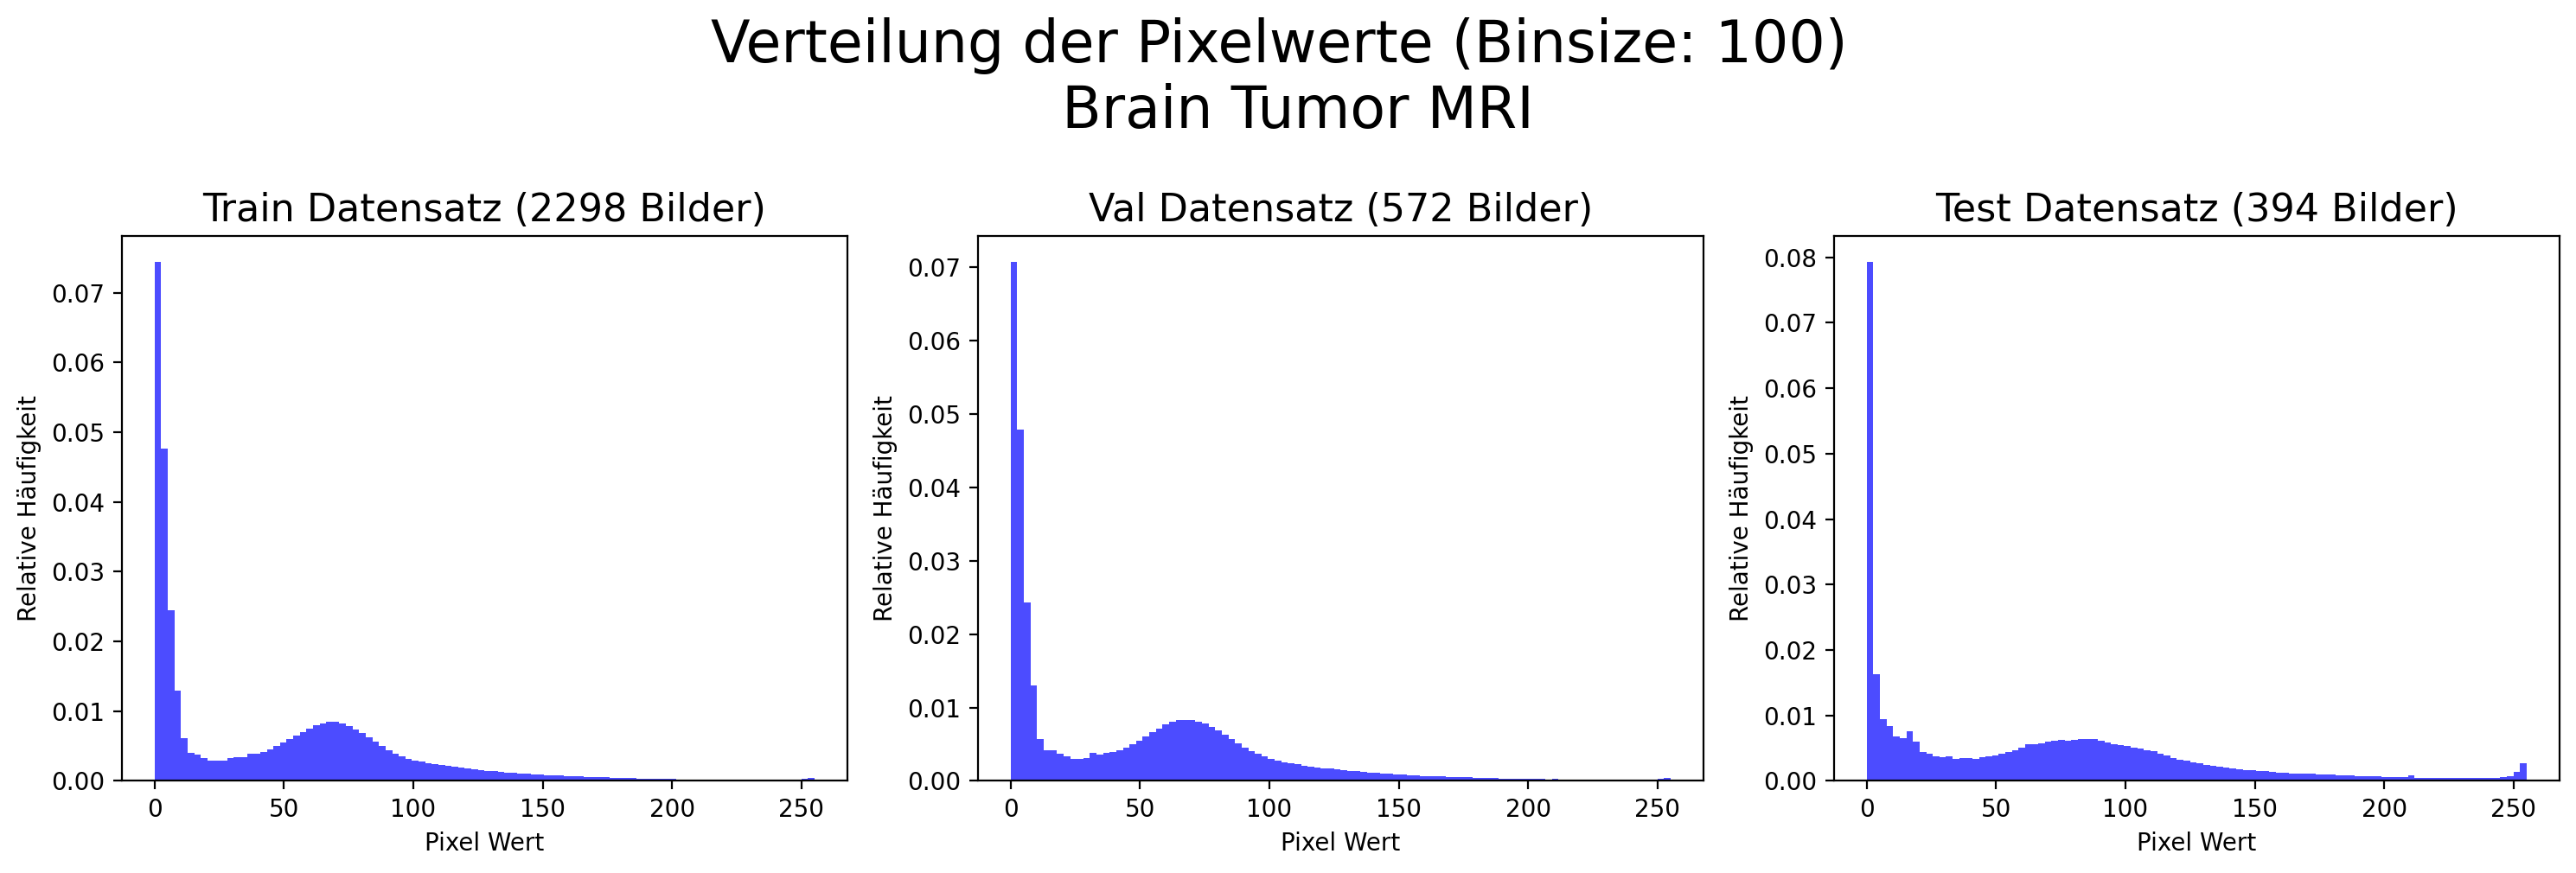
\includegraphics[width=\linewidth, height=5cm]{01-images/03-data/brain-Pixelverteilung-Partitionen.png}
    \caption{Histogramme der Pixelverteilung von Hirntumor in jeder Datenpartition}
    \label{fig:hist-datapartition-brain}
\end{figure}

Ein ähnliches Muster, das durch einen deutlichen Buckel gekennzeichnet ist, zeigt sich auch in diesem Hirntumor-Datensatz, jedoch mit einer Peakverschiebung. In den Hirntumor Histogrammen tritt dieser Peak typischerweise bei einem Pixelwert von etwa 80 auf. Sowohl die Trainings- als auch die Validierungspartition weisen ein vergleichbares Muster auf. In der Testpartition ist der Buckel allerdings weniger stark ausgeprägt. Zudem kommt es ab einem Pixelwert von 250 zu einem markanten Anstieg, der am Ende des Histogramms einen signifikanten Ausschlag verursacht. Eine mögliche Erklärung, dass die Testdatenpartition aus einer anderen Verteilung kommt. 

\subsubsection{Differenzbilder} \label{chap:Differenzenbilder-TestProblemEda2-mri}

Auch bei den Differenzbilder ist das Vorgehen, analog wie im Kapitel \ref{chap:Differenzenbilder-TestProblemEda2-covidx} beschrieben. 

\begin{figure}[ht]
    \centering
    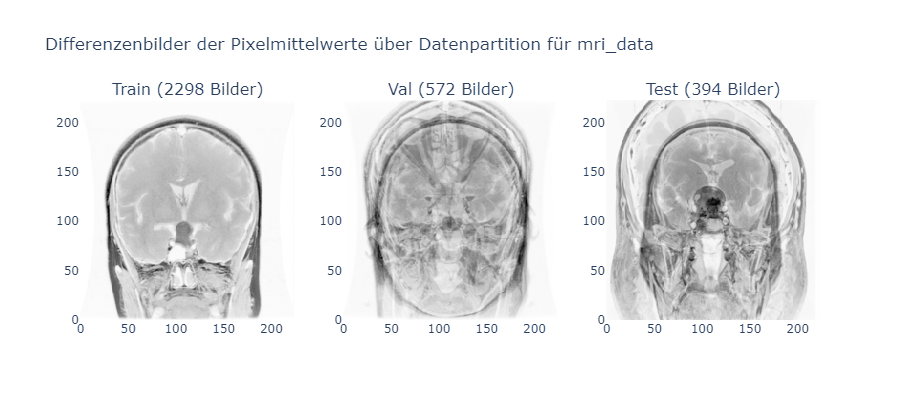
\includegraphics[width=\linewidth, height=5cm]{01-images/03-data/brain-Differenzenbilder-Partition.png}
    \caption{Differenzbilder von Hirntumor in jeder Datenpartition}
    \label{fig:differenzenbilder-datapartition-brain}
\end{figure}

In der Trainingspartition der Differenzbilder ist eine klare und detaillierte Konsistenz der Bilder vorhanden. In der Validierungs- und Testpartition ist dies jedoch nicht der Fall. Dort sind verschwommene Darstellungen zu erkennen, was auf die unterschiedliche Vielfalt der Bilder zurückzuführen ist. Dabei lässt sich visuell feststellen, dass die Verschwommenheit in der Validierungspartition nicht so stark ausgeprägt ist wie in der Testpartition.

\subsubsection{Feature Maps \& PCA} \label{chap:FeatureMaps-TestProblemEda3-mri}

\todo{Im Anhang hinzufuegen ? }

\newpage

% Methodik
\section{Methodik} 
In diesem Abschnitt werden die in dieser Thesis angewandten Methoden erläutert, einschliesslich der verwendeten Modelle, Metriken und Algorithmen.

\subsection{Technische Umsetzung} \label{chap:technische-umsetzung}
Für die technische Umsetzung dieser Bachelorarbeit wurden bewährte Data Science Frameworks verwendet, darunter Numpy, Pandas, Matplotlib und Seaborn. Für die Modellierung und Bildverarbeitung kamen PyTorch und PyTorch-Lightning zum Einsatz. Der Trainingsprozess sowie die Modelle wurden mit Weights \& Biases verfolgt.

\subsection{Preprocessing}  \label{chap:preprocessing}
Das Preprocessing transformiert die Rohdaten, dass sie optimal für das Training oder die Verarbeitung durch das Modell vorbereitet sind. Dieser Abschnitt behandelt zwei Arten des Preprocessings, Preprocessing beim Training und Preprocessing mit Perturbationen.

\subsubsection{Preprocessing beim Training} \label{chap:Preprocessing beim Training}
Alle Bilder werden beim Training durch eine Preprocessing Pipeline vorbereitet. Dabei werden die Bilder auf eine Grösse von 224 x 224 Pixel mit Antialiasing skaliert.

Antialiasing ist eine Technik, die in der Computergrafik verwendet wird, um den Aliasing-Effekt zu entfernen. Der Aliasing-Effekt führt zu gezackten Kanten in gerasterten Bildern.

\subsubsection{Preprocessing mit Perturbation} \label{chap:Preprocessing mit Perturbation}
Die erzeugten Perturbationen werden durch eine elementweise Addition auf den Inputbildern hinzugefügt. Die Addition der Perturbationen kann durch das Erstellen eigener PyTorch-Custom-Preprocessing-Klassen codiert werden, was eine einfache Integration in die Adversarial Training Pipeline ermöglicht. 

\subsection{Klassifikationsmodelle} \label{chap:klassifikationsmodelle}
In dieser Thesis wurde die Generalisierbarkeit verschiedener Klassifikationsmodelle in unterschiedlichen Architekturen untersucht. Dazu wurden die durch die PyTorch Library bereitgestellt Modelle ResNet \cite{he_deep_2015}, DenseNet \cite{huang_densely_2018}, EfficientNetV2, \cite{tan_efficientnetv2_2021} AlexNet, \cite{krizhevsky_imagenet_2012}, VGG \cite{simonyan_very_2015} und der \acrfull{vit} \cite{dosovitskiy_image_2021} verwendet. In jeder Modellfamilie wurden zwei bis drei Modelle trainiert und evaluiert. Durch die Vielfalt der verwendeten Modelle wird sichergestellt, dass die Ergebnisse nicht auf eine spezifische Architektur beschränkt sind. Modelle, die kein erfolgreiches Training durchliefen, wurden aussortiert und nicht weiter berücksichtigt. Betroffen waren unter anderem die Modellfamilien AlexNet, VGG und der \acrfull{vit}. Eine ausführlichere Darstellung hierzu befindet sich im Kapitel \ref{chap:ergebnisse-modelltraining}.

Bei der Berechnung der Metriken, der Generation der Perturbationen und der \Gls{robustifizierung} des Modells, wird in dieser Arbeit jegliches Modell als $f(\cdot)$ referenziert.

\subsubsection{ResNet}
Das ResNet oder Residual Neural Network wurde von Kaiming et al. \cite{he_deep_2015} entwickelt und erreichte einen Fehler von 3.57\% auf dem ImageNet-Testdatensatz. Dieses Ergebnis führte zum Sieg in der Klassifikationsaufgabe des ILSVRC 2015. Beim ResNet werden Residual Connections eingesetzt, um sogenannte ``Skip Connections'' zwischen den Konvolutionen des neuronalen Netzwerks zu etablieren. Diese Verbindungen erleichtern den direkten Fluss von Informationen zwischen den Konvolutionen, was das Problem des Vanishing Gradient während des Trainings verhindert. Durch die Residual Connections können tiefe neuronale Netzwerke effektiver trainiert werden, da sie den Gradientenfluss durch das Netzwerk erleichtern.

\subsubsection{DenseNet}
Das DenseNet, kurz für Densely Connected Convolutional Networks, wurde von Huang et al. \cite{huang_densely_2018} eingeführt und stellt eine Weiterentwicklung des ResNet dar. Im Gegensatz zum ResNet, das Skip Connections zwischen bestimmten Konvolutionen herstellt, implementiert DenseNet eine dichte Verbindungsstruktur innerhalb sogenannter ``Dense Blocks''. In diesen Blöcken ist jede Konvolution direkt mit allen nachfolgenden Konvolutionen verbunden. Zwischen den Dense Blocks befinden sich Übergangsschichten, die für Dimensionsreduktion sorgen. Diese Struktur ermöglicht eine effiziente Informationsübertragung und fördert die Wiederverwendung von Merkmalen innerhalb des Netzwerks. Durch die direkten Verbindungen sowohl innerhalb als auch zwischen den Dense Blöcken kann DenseNet den Informationsverlust während des Trainings reduzieren und die Stabilität des Gradientenflusses verbessern.

\subsubsection{EfficientNetV2} 
EfficientNetV2, vorgestellt von Tan et al. \cite{tan_efficientnetv2_2021}, ist eine Weiterentwicklung des EfficientNet-Modells, die darauf abzielt, ein optimales Gleichgewicht zwischen Modellgrösse und Leistung durch eine skalierbare Compound Scaling-Strategie zu erreichen. Im Gegensatz zu früheren Ansätzen berücksichtigt EfficientNetV2 neben Tiefe, Breite und Auflösung auch die Netzwerkstruktur und verwendet verbesserte Bausteine wie EfficientConv, eine effizientere Variante der Standard-Konvolution. Diese Verbesserungen ermöglichen es dem Modell, mit weniger Parametern vergleichbare oder sogar bessere Leistungen bei verschiedenen Bilderkennungsaufgaben zu erzielen als andere Modelle. Die resultierende Effizienz macht EfficientNetV2 zu einer attraktiven Wahl für ressourcenbeschränkte Umgebungen oder Anwendungen, die schnelle Inferenzzeiten erfordern.

\subsection{Metriken}
\todo{Write small introduction text}

\subsubsection{Confusion matrix}

Die Confusion Matrix ist ein Werkzeug, das verwendet wird, um die Vorhersagen eines Klassifikationsmodells mit der tatsächlichen Wahrheit zu vergleichen. Dabei werden die Vorhersagen des Modells in vier Kategorien unterteilt:

\begin{enumerate}
    \item True Positives (TP): Elemente, die korrekterweise als zur Zielklasse gehörend erkannt wurden.
    \item True Negatives (TN): Elemente, die korrekterweise als nicht zur Zielklasse gehörend erkannt wurden.
    \item False Positives (FP): Elemente, die fälschlicherweise als zur Zielklasse gehörend vorhergesagt wurden, obwohl sie es in Wirklichkeit nicht sind.
    \item False Negatives (FN): Elemente, die fälschlicherweise nicht als zur Zielklasse gehörend erkannt wurden, obwohl sie es eigentlich sind.
\end{enumerate}

Nachfolgende die Darstellung einer Confusion Matrix, mit der Anordnung von PyTorch Torchmetrics. 

\begin{table}[h]
    \centering
    \begin{tabular}{l|l|c|c|}
        \multicolumn{2}{c}{}&\multicolumn{2}{c}{Predicted label}\\
        \cline{3-4}
        \multicolumn{2}{c|}{}&Negativ&Positiv\\
        \cline{2-4}
        \multirow{2}{*}{Actual label}& Negativ & $TN$ & $FP$\\
        \cline{2-4}
        & Positiv & $FN$ & $TP$\\
        \cline{2-4}
    \end{tabular}
    \label{tab:conftable}
    \caption{Binäre Konfusionsmatrix}
\end{table}

\subsubsection{Precision}
Precision (Präzision) misst das Verhältnis der korrekt identifizierten positiven Instanzen zu allen Instanzen, die vom Modell als positiv klassifiziert wurden. Mit anderen Worten, Precision gibt an, wie viele der als positiv identifizierten Fälle tatsächlich positiv sind. Die Formel für Precision ist:

\begin{equation}
    \text{Precision} = \frac{TP}{TP + FP}
    \label{eq:PrecisionFormula}
\end{equation}


\subsubsection{Recall}

Recall hingegen misst das Verhältnis der korrekt identifizierten positiven Instanzen zu allen tatsächlich positiven Instanzen. Mit anderen Worten, Recall gibt an, wie viele der tatsächlich positiven Fälle vom Modell korrekt identifiziert wurden. Die Formel für Recall ist:

\begin{equation}
    \text{Recall} = \frac{TP}{TP + FN}
    \label{eq:RecallFormula}
\end{equation}

\subsubsection{Specificity}
Specificity ist eine weitere wichtige Metrik zur Bewertung der Leistung von Klassifizierungsmodellen. Im Gegensatz zu Precision und Recall, die sich auf die Leistung des Modells bei der Identifizierung von positiven Instanzen konzentrieren, misst die Spezifität die Fähigkeit des Modells, negative Instanzen korrekt zu identifizieren.

Die Spezifität gibt das Verhältnis der korrekt identifizierten negativen Instanzen zur Gesamtzahl der tatsächlich negativen Instanzen an. Anders ausgedrückt, Spezifität gibt an, wie viele der tatsächlich negativen Fälle vom Modell korrekt identifiziert wurden. Die Formel für Spezifität ist:

\begin{equation}
    \text{Specificity} = \frac{TN}{TN + FP}
    \label{eq:SpecificityFormula}
\end{equation}

\subsubsection{AUROC}
Die AUROC (Area Under the Receiver Operating Characteristic Curve) ist eine Metrik zur quantitativen Bewertung der Leistungsfähigkeit von Klassifizierungsmodelle. Die zugrundeliegende ROC-Kurve (Receiver Operating Characteristic Curve) visualisiert das Verhältnis zwischen der True Positive Rate (TPR) und der False Positive Rate (FPR) eines Klassifizierungsmodells über verschiedene Schwellenwerte für die Klassifikation. Hierbei variiert die TPR als Prozentsatz der korrekt identifizierten positiven Fälle im Verhältnis zur Gesamtzahl der tatsächlich positiven Fälle, während die FPR den Anteil der fälschlicherweise als positiv klassifizierten Fälle im Verhältnis zur Gesamtzahl der tatsächlich negativen Fälle beschreibt.

\begin{equation}
    \text{True Positive Rate (TPR)} = \text{Recall} =\frac{\text{TP}}{\text{TP} + \text{FN}}
    \label{eq:TPR}
\end{equation}

\begin{equation}
    \text{False Positive Rate (FPR)} = \frac{\text{FP}}{\text{FP} + \text{TN}} 
    \label{eq:FPR}
\end{equation}

Die AUROC quantifiziert die Gesamtleistung des Klassifizierungsmodells, indem sie die Fläche unter der ROC-Kurve berechnet. Ein Wert von 0.5 deutet auf ein schlechtes Modell hin, das äquivalent zu einer zufälligen Klassifikation ist, während ein Wert von 1 eine perfekte Klassifikation ohne Fehler bedeutet. Die AUROC ermöglicht somit eine quantiative Vergleichbarkeit verschiedener Klassifizierungsmodelle.


\subsubsection{F1-Score}
Der F1-Score ist eine Metrik, die Precision und Recall kombiniert, um die Gesamtleistung eines Klassifizierungsmodells zu bewerten. Er ist besonders nützlich, wenn ein ausgewogenes Verhältnis zwischen Precision und Recall angestrebt wird.

Der F1-Score wird als harmonisches Mittelwert von Precision und Recall berechnet und berücksichtigt sowohl falsch positive als auch falsch negative Vorhersagen. Die Formel für den F1-Score lautet:

\begin{equation}
    \text{F1} = 2 \cdot \frac{Precision \cdot Recall}{Precision + Recall}
    \label{eq:F1Score}
\end{equation}

Durch die Berücksichtigung von Precision und Recall ermöglicht der F1-Score eine umfassendere Bewertung der Leistung eines Klassifizierungsmodells. Ein hoher F1-Score zeigt an, dass das Modell sowohl eine hohe Precision als auch einen hohen Recall aufweist, was darauf hindeutet, dass es sowohl präzise als auch umfassend bei der Identifizierung von positiven Instanzen ist.

Der F1-Score ist besonders nützlich in Situationen, in denen ein Ungleichgewicht zwischen den Klassen vorliegt oder wenn sowohl Precision als auch Recall von Bedeutung sind, wie zum Beispiel bei der Erkennung von Betrug oder bei medizinischen Diagnosen.


\subsubsection{Fooling Rate}
Die Fooling Rate beschreibt, wie erfolgreich ein Modell durch adversarial Attacks getäuscht werden kann. Sie misst den relativen Anteil der erfolgreichen Attacken, das das Modell falsch klassifiziert hat. Zum Beispiel, wenn ein Modell eine Fooling Rate von 80\% hat, bedeutet das, dass von 100 modifizierten Bildern 80 fälschlicherweise klassifiziert werden. Eine hohe Fooling Rate bedeutet, dass das Modell anfälliger für adversarielle Angriffe ist und somit weniger vertrauenswürdig in Bezug auf die Klassifizierung von Daten. Mathematisch lässt sich die Fooling Rate wie folgt definieren. 

\begin{equation}
    \text{Fooling Rate} = \frac{1}{N} \sum_{i=1}^{N} \left\{ \begin{array}{ll} 1, & \text{if } \text{round}(\hat{y}_i) \neq \text{round}(\hat{y}_{adv,i}) \\ 0, & \text{otherwise} \end{array} \right.
    \label{eq:Fooling Rate}
\end{equation}

Wobei die Funktion Rundungsfunktion $\text{round}(\cdot)$ wie folgt definiert ist:

\todo{should we define things like x is real}

\begin{equation}
    \text{round}(x) = \lfloor x + 0.5 \rfloor \quad \text{, } x \in \mathbb{R}
    \label{eq:Rundungsfunktion}
\end{equation}


\subsubsection{Matrizennorm}
\todo{Brauchen wir das so genau erklärt?}
Vektoren repräsentieren nicht nur Richtungen, sondern auch Längen. Diese Längenmessung wird durch die sogenannte Norm ermöglicht. Für einen Vektor $v$ wird die Norm wie folgt berechnet:

\begin{equation}
    \| v \| = \sqrt{\sum_{i=1}^{n} v_i^2}
    \label{eq:Vektornorm}
\end{equation}

Matrizen sind eine Erweiterung dieses Konzepts. Ähnlich wie bei Vektoren können wir die "`Grösse"' einer Matrix mit einer entsprechenden Norm messen. Die Norm einer Matrix $A$ wird durch die Formel definiert:

\begin{equation}
    \| A \|_P = \sqrt{\sum_{i=1}^{m} \sum_{j=1}^{n} |a_{ij}|^p}
    \label{eq:Matrixnorm}
\end{equation}

Hier steht $p$ für einen Parameter, der die Art der Norm festlegt. Beispielsweise entspricht $p=2$ der Frobeniusnorm. Wenn $p$ gegen unendlich kovergiert, erhalten wir die Maximumnorm, die den höchsten Wert in der Matrix entspricht:

\begin{equation}
    \|A\|_{\infty} = \max_{1 \leq i \leq m} \sum_{j=1}^{n} |a_{ij}|
    \label{eq:Maximumnorm}
\end{equation}

Diese Definitionen helfen uns, die "`Grösse"' von Matrizen in verschiedenen Kontexten zu verstehen und zu quantifizieren.
\subsection{Modell Training} \label{chap:modelltraining}
In diesem Kapitel wird erläutert, wie die Baseline-Modelle trainiert werden und welche Komponenten dabei zum Einsatz kommen.

\subsubsection{Loss-Funktion} \label{chap:loss-function}
Das Modelltraining nutzt den \acrfull{bce} Loss. Der \acrshort{bce} Loss wird minimiert, wenn das Modell eine perfekte Vorhersage trifft (d.h. wenn $\hat{y}_i = y_i$ für alle $i$) und steigt, je weiter $\hat{y}_i$ von $y_i$ abweicht.

Der \acrshort{bce} Loss ist definiert als:

\begin{equation}
    L_{\text{BCE}} = -\frac{1}{N} \sum_{i=1}^{N} (y_i \cdot \log(\hat{y}_i) + (1-y_i) \cdot \log(1-\hat{y}_i))
    \label{eq:TrainingBCE}
\end{equation}

\begin{align*}
    y_i,        &\text{ Label des $i$-ten Datenpunkts.} \\
    \hat{y}_i,  &\text{ Vorhersage des Modells des $i$-ten Datenpunkts.} \\
    N,          &\text{ Gesamtanzahl Datenpunkte.} \\
\end{align*} 

\subsubsection{Adam-Optimizer} \label{chap:optimizer}
Für die Optimierung der Modellparameter wird der Adam-Optimizer von Kingma et al. \cite{kingma_adam_2017} genutzt. Dieser Optimierungsalgorithmus wurde zur Anpassung stochastischer Zielfunktionen mittels Gradientenverfahren entwickelt. Er kombiniert Techniken wie Momentum und RMSprop, um die Lernrate dynamisch anzupassen und die Konvergenz des Modells zu verbessern. Adam-Optimizer zeigt in der Praxis gute Ergebnisse und ist mit anderen Methoden der stochastischen Optimierung vergleichbar.

\subsubsection{Hyperparamteroptimierung und Modellselektion}
Für das Training werden alle Datensätze und Modelle iteriert, die in den Kapitel \ref{chap:Daten} und \ref{chap:klassifikationsmodelle} beschrieben sind. Aufgrund der Grösse des \nameref{chap:COVIDx CXR-4}-Datensatzes im Vergleich zum \nameref{chap:Brain-Tumor} werden beim \nameref{chap:COVIDx CXR-4} Datensatz pro Trainingsepoche zufällig 5\% des Trainingssubsets ausgewählt. Für jede Kombination aus Datensatz und Modell werden drei Trainingsdurchläufe gestartet, wobei für die Lernrate jeweils die drei Werte $10^{-5}$, $10^{-4}$ und $10^{-3}$ nacheinander verwendet werden.

Aufgrund des hohen Rechenaufwands und begrenzter Ressourcen wird auf eine Hyperparameteroptimierung bei der L2-Regularisierung und dem Dropout vor dem letzten Klassifikationslayer verzichtet. Stattdessen wird der beste Checkpoint jeder Modell-Datensatz-Kombination basierend auf dem niedrigsten Validierungsloss gespeichert.
\subsection{UAP Algorithmus} \label{chap:UAP}

Der hier beschriebene Algorithmus für die Generation von einer \acrfull{uap} basiert auf dem Ansatz von Moosavi-Dezfooli et al. \cite{moosavi-dezfooli_universal_2017}. Ziel ist, eine Perturbation zu entwickeln, die auf neue Bilder übertragbar ist. Der Algorithmus durchläuft iterativ eine Auswahl von Trainingsbildern und findet jeweils den kürzesten Weg zur Entscheidungsgrenze jedes Bildes. Dabei werden die erzeugten Perturbationen aufsummiert, um eine universelle Perturbation zu erzeugen.

Bei der Generation der \acrshort{uap}s wird nur eine Teilmenge der positiv gelabelten Trainingsbilder verwendet. Die generierten \acrshort{uap}s sind speziell darauf ausgelegt, positive Klassenbilder fälschlicherweise als negative zu klassifizieren.

\subsubsection{Loss-Funktion $L_{\text{UAP}}$}
Das Optimierungsproblem des Referenzpapers \cite{moosavi-dezfooli_universal_2017} wird in dieser Implementierung durch eine selbst definierte Loss-Funktion gelöst, welche die Norm der Perturbationstensor und die inverse \acrlong{bce} Funktion minimiert. Durch die Minimierung der Norm der Perturbationstensor wird sichergestellt, dass die erzeugte Perturbation minimal ist und somit weniger auffällig. Gleichzeitig sorgt die Minimierung der Inverse \acrlong{bce} dafür, dass die aktuelle Perturbation an die Entscheidungsgrenze bringt. Diese doppelte Optimierung stellt sicher, dass die Perturbationen sowohl klein als auch wirksam ist.

% Die Grundidee dabei ist, dass die Norm die aktuelle Perturbation so klein wie möglich hält und die Inverse der \acrlong{bce} die aktuelle Perturbation an die Entscheidungsgrenze bringt.

Die Loss-Funktion optimiert den Tensor $\Delta v$ und sieht wie folgt aus:
\begin{equation}
    L_{UAP} = \lambda_{norm} \cdot ||v + \Delta v||_p + \frac{1}{L_{BCE}(\hat{y}, \hat{y}_{\text{adv}}) + \epsilon}
\label{Loss}
\end{equation}

Wobei die verwendete \acrlong{bce} wie folgt minimiert wird:
\begin{equation}
L_{BCE} = - (\hat{y} \cdot \log(\hat{y}_{\text{adv}}) + (1-\hat{y}) \cdot \log(1-\hat{y}_{\text{adv}}))
\label{eq:BCE}
\end{equation}

\begin{align*}
%\text{wobei:}&\\
L_{UAP}, &\text{ ist der gesamte Loss.} \\
L_{BCE}, &\text{ bezeichnet den \acrlong{bce} Loss.} \\
\lambda_{norm}, &\text{ ist der Regularisierungsparameter der Matrizennorm.} \\
v, &\text{ ist die universelle adversarial Perturbation.} \\
\Delta v, &\text{ ist die Änderung der Perturbation } v \text{.} \\
||v + \Delta v||_p, &\text{ repräsentiert die } L_p \text{-Norm der Perturbation } v + \Delta v. \\
\hat{y}, &\text{ ist die Vorhersage des Modells für das Originalbild ($\text{img}$).} \\
\hat{y}_{adv}, &\text{ ist die Vorhersage des Modells für das perturbierte Bild ($\text{img} + v + \Delta v$).} \\
\epsilon, &\text{ ist eine kleine positive Konstante für numerische Stabilität.}
\end{align*}

Der Algorithmus erfordert eine Batch Size von 1 und führt nach jeder Berechnung die Backpropagation durch, wodurch kein Mittelwert bei der Loss-Funktion berechnet wird. $\hat{y}$ sowie $\hat{y}_{adv}$ beziehen sich auf das aktuelle Bild im Algorithmus.

Für $\epsilon$ wird ein kleiner Wert wie $10^{-6}$ gewählt, der eine Division durch 0 verhindert, wenn der Output unseres Modells sowohl mit als auch ohne Perturbation gleich ist. Dies ist vor allem bei der Berechnung der ersten Perturbation ein Problem, da zu diesem Zeitpunkt ein Nulltensor vorhanden ist.

\subsubsection{Technische UAP Umsetzung} \label{chap:technische_umsetzung_uap}

Die technische Umsetzung des Prozesses zur Generierung der \acrshort{uap} Bilder ist im folgenden Pseudocode visualisiert.



\begin{algorithm}[H]
\caption{Algorithmus für die Generierung von \acrlong{uap}}
\begin{algorithmic}[1]
\label{algo:UAP Algorithmus}
\STATE \textbf{initialize} Liste $v$
\FOR{Anzahl Perturbationen $i$}
    \STATE \textbf{initialize} Nulltensor $v_i$
    \WHILE{$\text{Fooling Rate}(k) < r$}
        \FOR{$\text{img}$ in Trainingsdatensatz $X_{1:n}$}
        \STATE \textbf{initialize} Nulltensor $\Delta v$
        \STATE \textbf{initialize} $j_{\text{tries}} \gets 0$
            \WHILE{$(\hat{y}_{(img)} \geq k) = (\hat{y}_{({\text{img} + v_i + \Delta v})} \geq k)$ \textbf{and} $j_{\text{tries}} < t$}         
            \STATE Aktualisiere $\Delta v$ mittels $L_{\text{UAP}}$: $$\Delta v \gets \Delta v - lr_{\text{UAP}} (\frac{\partial L_{UAP}}{\partial \Delta v})$$
            \STATE Inkrementiere $j_{\text{tries}}$: $$j_{\text{tries}} \gets j_{\text{tries}} + 1$$
            \ENDWHILE
            \STATE Addiere die Perturbation $\Delta v$ auf $v_i$: $$v_i \leftarrow v_i + \Delta v$$
        \ENDFOR
    \ENDWHILE
    \STATE Füge $v_i$ zur Liste $v$ hinzu
\ENDFOR
\STATE \textbf{return} Liste von Perturbationen $v$
\end{algorithmic}
\end{algorithm}

\text{Wobei man folgende Parameter selbst bestimmen muss:}
\begin{align*}
i, &\text{ ist die Anzahl Perturbationsbilder, welche generiert werden.} \\
n, &\text{ ist die Anzahl Trainingsbilder, welche für die Generierung verwendet werden.} \\
t, &\text{ ist die Anzahl Versuche, eine bildlokale Perturbation zu finden.}\\
X_{1:n}, &\text{ ist eine Teilmenge aller positiven gelabelten Trainingsbilder.} \\
r, &\text{ ist der prozentuelle Anteil von Trainingsbilder, welche durch die Perturbationen} \\ 
&\text{  getäuscht werden, damit die Perturbation } v_i \text{ gespeichert wird.} \\
k, &\text{ ist der Threshold der Entscheidungsgrenze.} \\
p, &\text{ ist der Normparameter der $L_p$ Norm, siehe \nameref{Loss}.}\\
\lambda_{norm},\epsilon, &\text{ siehe \nameref{Loss}.}\\
lr_{\text{UAP}}, &\text{ ist die Learningrate für die Gewichtsaktualisierung von $\Delta v$.}
\end{align*}

Eine visuelle Darstellung zum \Gls{algorithmus} ist bei Abbildung \ref{fig:05-uap_algorithm} im Anhang zu finden. 

\subsubsection{Wahl des Matrizennormregularisierungsparameters $\lambda_{norm}$}

In Vorversuchen wurde festgestellt, dass jedes Modell standardmässig unterschiedlich robust gegenüber \acrshort{uap}s ist und dass der Matrizennormalisierungsparameter $\lambda_{norm}$ nicht universell gewählt werden kann. Wenn dieser Parameter zu hoch gewählt wird, wird die Perturbationsgenerierung für manche Modelle instabil und die gewünschte Schwelle der Entscheidungsgrenze $k$ kann nicht erreicht werden. Daher muss vor jeder Robustifizierung für jedes Modell manuell ein stabiler Regularisierungsparameter $\lambda_{norm}$ gefunden werden. Je höher dieser gewählt wird, desto instabiler ist die Generierung der \acrshort{uap}s, aber desto geringer ist die Perturbation.
\\
\\
In der folgenden Tabelle \ref{tab:Matrizennormregularisierungsparameter} werden einige der gewählten Werte erfasst:

\begin{table}[h!]
\centering
\begin{tabular}{l|l|l}
\hline
\textbf{Datensatz} & \textbf{Modell} & \textbf{$\lambda_{norm}$} \\ 
\hline
MRI & ResNet50 & $0.05$ \\
\hline
'' & ResNet18 & $>$1 \\
\hline
COVIDx & - & - \\
\hline
'' & - & - \\
\bottomrule
\end{tabular}
\caption{Beispiele der gewählten Matrizennormregularisierungsparameter $\lambda_{norm}$}
\label{tab:Matrizennormregularisierungsparameter}
\end{table}

\todo{Befüllen}
\subsection{Schutzmechanismen}

Im Kapitel Schutzmechanismen listen wir Mechanismen auf, welche wir testen, um unsere in Kapitel \ref{chap:modelltraining} beschriebenen Modelle robuster gegen adversariale Angriffe machen sollen.

\subsubsection{Adversarial Training} \label{chap:adversarial training}

Die Grundidee hinter Adversarial Training ist, dass wir Perturbationen generieren und unser Modell auf diesen Perturbationen iterativ weitertrainieren. Wir hoffen, dass das Modell beim Weitertrainieren die Entscheidungsgrenze für mögliche Perturbationen weiter vom Nullpunkt verschiebt. Dadurch müssen diese Perturbationen grösser werden, um das Modell zu täuschen.

\begin{figure}[H]
    \centering
    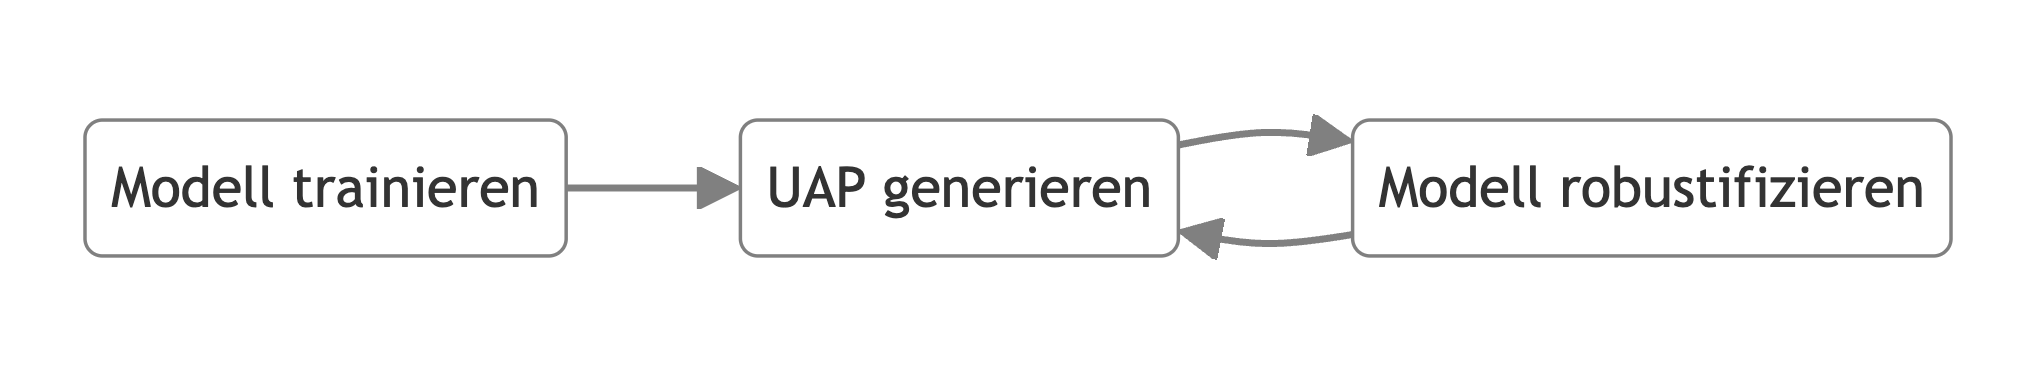
\includegraphics[width=13.5cm]{01-images/04-methodik/simplified_overview.png}
    \caption{Simplifizierte Version unseres Vorgehens}
    \label{fig:07-simplified_overview}
\end{figure}

In der Abbildung \ref{fig:Evaluierungspipeline} ist der Iterationsschritt der Pipeline zu sehen. 

\begin{figure}[H]
    \centering
    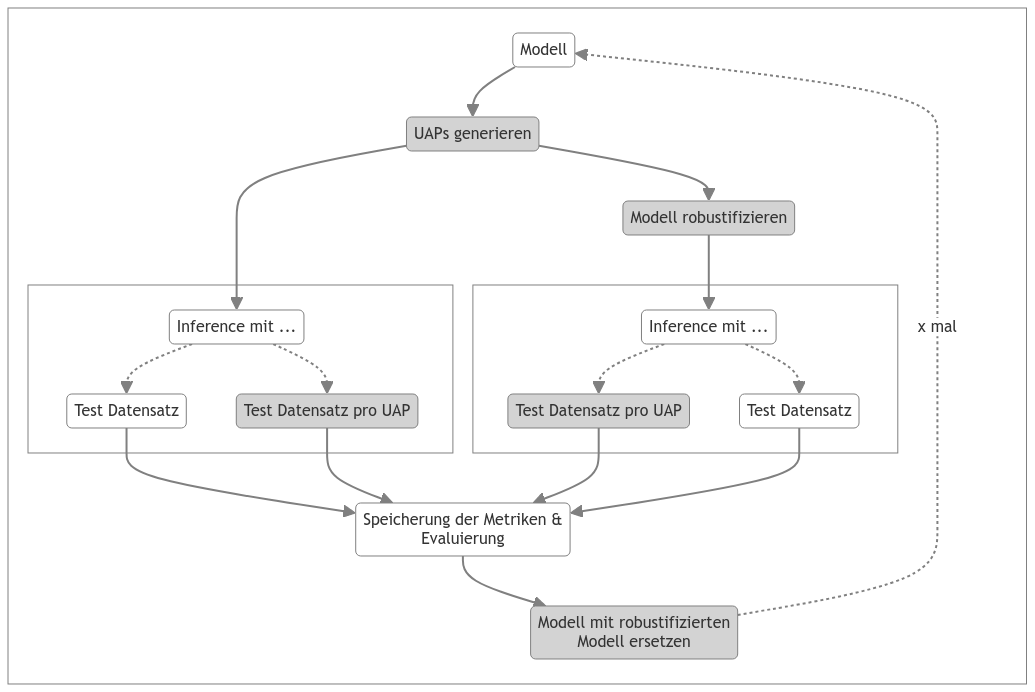
\includegraphics[width=\linewidth]{01-images/04-methodik/robustifizierungs-pipeline.png}
    \caption{Übersicht der Evaluierungspipeline}
    \label{fig:Evaluierungspipeline}
\end{figure}


\begin{itemize}
    \item \textbf{Modell}: Das vortrainierte Modell, welches robustifiziert wird.
    \item \textbf{UAPs generieren}: \acrshort{uap} werden generiert, um das Modell robuster zu machen.
    \item \textbf{Modell robustifizieren}: Adversarial Training wird angewendet, um das Modell zu robustifizieren. Siehe Kapitel \ref{chap:adversarial training}.
    \item \textbf{Inference mit...}: Erfolgt über zwei parallele Wege:
        \begin{itemize}
            \item Einer führt zur Inferenz mit dem ursprünglichen Modell, jeweils für den Testdatensatz mit und ohne \acrshort{uap}.
            \item Der andere Weg führt zur Inferenz mit dem robustifizierten Modell, ebenfalls für Testdatensatz mit und ohne \acrshort{uap}.
        \end{itemize}
    \item \textbf{Speicherung der Metriken \& Evaluierung}: Hier speichern wir die berechneten Metriken und vergleichen die vier Outputs der Inferenz miteinander untereinander für jede Robustifikations Iteration. 
\end{itemize}

\newpage

Technisch lässt sich unsere Pipeline so umsetzen:

\begin{algorithm}
\caption{Pipeline zur Generierung von universelle adversarial Perturbationen}
\label{alg:UAP_Pseudo_Algorithmmus}
\begin{algorithmic}[1]
\STATE Modell laden
\FOR{Anzahl Robustifizierungen n\_robustifications}
    \STATE Generierung der UAPs (Algorithmus \ref{algo:UAP Algorithmus})
    \STATE Inferenz auf den Testdaten ($p_{\text{adv}}$=0.0)
    \FOR{jede UAP}
        \STATE Inferenz auf den Testdaten mit UAP ($p_{\text{adv}}$=1.0)
    \ENDFOR
    \STATE Modelltraining mittels UAPs (random selection, $p_{\text{adv}}$=0.5)
    \STATE Laden des besten Modellcheckpoints
    \STATE Inferenz auf den Testdaten mit dem robustifiziertem Modell ($p_{\text{adv}}$=0.0)
    \FOR{jede UAP}
        \STATE Inferenz auf den Testdaten mit UAP mit dem robustifizierem Modell ($p_{\text{adv}}$=1.0)
    \ENDFOR
\ENDFOR
\end{algorithmic}
\end{algorithm}

\text{Wobei man folgende Parameter selbst bestimmen muss:}
\begin{align*}
\text{model}, &\text{ ist das Modell, welches robustifiziert werden soll.} \\
\text{dataset}, &\text{ ist der Datensatz, welcher zur robustifizierung genutzt werden soll.} \\
\text{n\_robustifications}, &\text{ ist die Anzahl Robustifizierungen, welche probiert werden sollten.} \\
i, &\text{ siehe Algorithmus \ref{algo:UAP Algorithmus}.}\\
n, &\text{ siehe Algorithmus \ref{algo:UAP Algorithmus}.}\\
t, &\text{ siehe Algorithmus \ref{algo:UAP Algorithmus}.}\\
r, &\text{ siehe Algorithmus \ref{algo:UAP Algorithmus}.}\\
k, &\text{ siehe Algorithmus \ref{algo:UAP Algorithmus}.}\\
p, &\text{ siehe Algorithmus \ref{algo:UAP Algorithmus}.}\\
\lambda_{norm}, &\text{ siehe Algorithmus \ref{algo:UAP Algorithmus}.}\\
\epsilon, &\text{ siehe Algorithmus \ref{algo:UAP Algorithmus}.}\\
\end{align*}

Hier bezieht sich $p_{\text{adv}}$ auf die Wahrscheinlichkeit, dass eine Perturbation beim Trainingsprozess oder bei der Inferenz auf das Bild addiert wird. Im Trainingsprozess beträgt die $p_{\text{adv}}$ bei der Validierung ebenfalls 0.5. Währenddessen nimmt die Inferenz auf den Testdaten Werte von entweder 0 oder 1 an. 


\subsubsection{Data Augmentation}

Bei der Data Augmentation verändern wir mit einer zufälligen Transformation die vorhandenen Trainingsdaten, um die Variabilität im Datensatz zu erhöhen. Dies kann durch verschiedene Methoden geschehen, wie zum Beispiel:

\begin{itemize}
    \item \textbf{Rotation}: Drehen des Bildes um einen bestimmten Winkel.
    \item \textbf{Verschiebung}: Verschieben des Bildes in eine bestimmte Richtung.
    \item \textbf{Skalierung}: Ändern der Grösse des Bildes.
    \item \textbf{Spiegelung}: Spiegeln des Bildes entlang einer Achse.
    \item \textbf{Rauschen hinzufügen}: Zufälliges Rauschen hinzufügen, um das Bild zu verändern.
\end{itemize}

Diese Techniken helfen, das Modell robuster zu machen und die Generalisierungsfähigkeit zu verbessern, indem sie es zwingen, verschiedene Variationen der Daten zu lernen.

\subsubsection{Input Ensembles}

Mit Input Ensembles nutzen wir mehrere Modelle, die unabhängig voneinander trainiert wurden. Der Prozess sieht wie folgt aus:

\begin{enumerate}
    \item \textbf{Training mehrerer Modelle}: Jedes Modell wird separat mit demselben Trainingsdatensatz trainiert.
    \item \textbf{Unabhängige Vorhersagen}: Jedes Modell gibt eine eigene Vorhersage, basierend auf dem Input.
    \item \textbf{Kombinieren der Vorhersagen}: Der endgültige Output wird durch Mehrheitsentscheidung (Voting) bestimmt. 
\end{enumerate}

Durch diese Methode können wir die Genauigkeit und Robustheit der Vorhersagen verbessern.

% Resultat
\section{Resultate}

\todo{Welche Grafiken sind sinnvoll}
\todo{Unsicherheiten und Straeungen}

\subsection{Ergebnisse des Modelltrainings}

\subsection{\acrlong{uap}}

\subsection{Anfälligkeit von ungeschützten Modellen}

\subsection{Anfälligkeit von geschützten Modellen}

\subsubsection{Data Augmentation}

\subsubsection{Adversarial Training}

\subsubsection{Input Ensembles}

\subsubsection{Weitere Verteidigungsmechanismen}

Detektion von Adversarial Bilder durch Bildanalysen, wie Fouriertransformation. 


\subsection{Universal Adversarial Perturbation}

\todo{Vergleiche mit anderen Perturbation oder mit Perturbationen aus dem UAP paper.}

\subsection{Anfälligkeit der ungeschützten Modelle}



\subsection{Anfälligkeit nach Adversarial Training}


%% ResNet
\subsubsection{UAP ResNet18}
\todo{Kapitel noch in Arbeit}
In diesem Kapitel visualisieren wir die UAP, welches durch das ResNet18 Modell erstellt wurden.

% UAPs Resnet18 covidx robustifikations level 0
\begin{figure}[ht!]
    \centering
    \begin{subfigure}{0.19\linewidth}
        \centering
        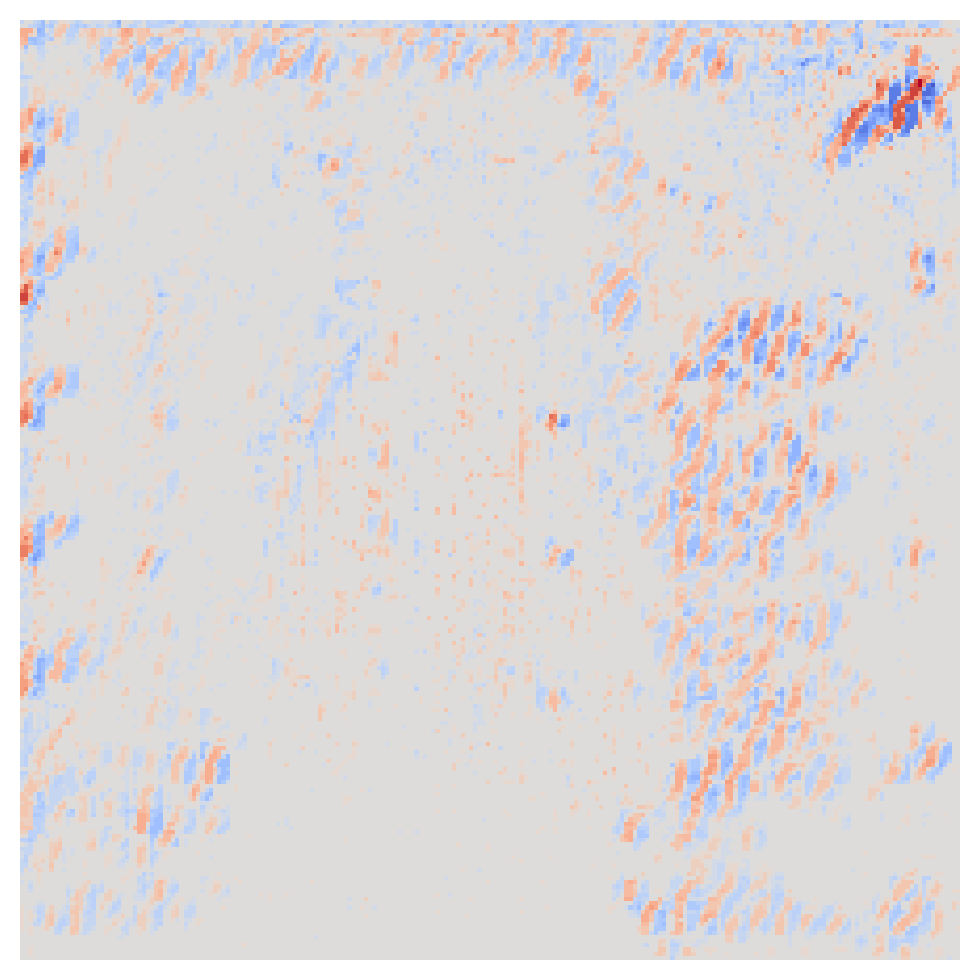
\includegraphics[height=1\linewidth]{01-images/05-resultate/uap_resnet/uap0-resnet18-covid-n200-robustificationslevel0.png}
        \caption{UAP Index 0}
    \end{subfigure}\hfill%
    \begin{subfigure}{0.19\linewidth}
        \centering
        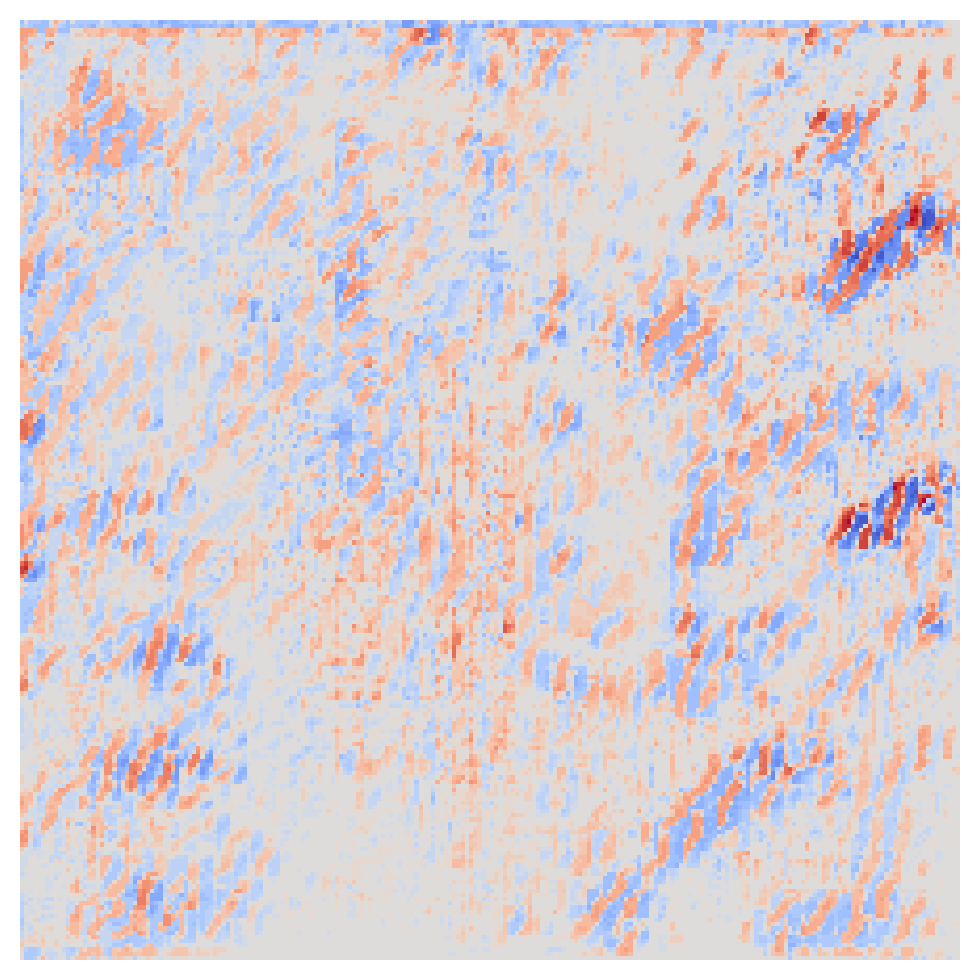
\includegraphics[height=1\linewidth]{01-images/05-resultate/uap_resnet/uap1-resnet18-covid-n200-robustificationslevel0.png}
        \caption{UAP Index 1}
    \end{subfigure}\hfill%
    \begin{subfigure}{0.19\linewidth}
        \centering
        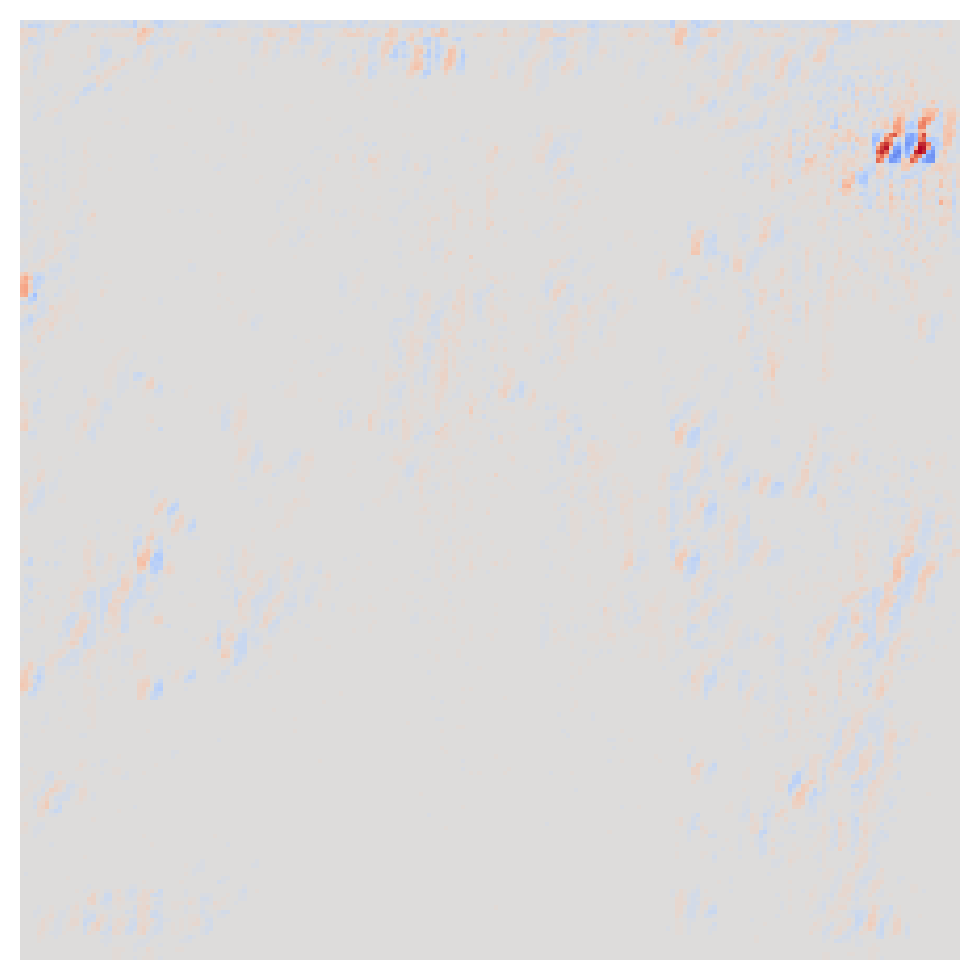
\includegraphics[height=1\linewidth]{01-images/05-resultate/uap_resnet/uap2-resnet18-covid-n200-robustificationslevel0.png}
        \caption{UAP Index 2}
    \end{subfigure}\hfill%
    \begin{subfigure}{0.19\linewidth}
        \centering
        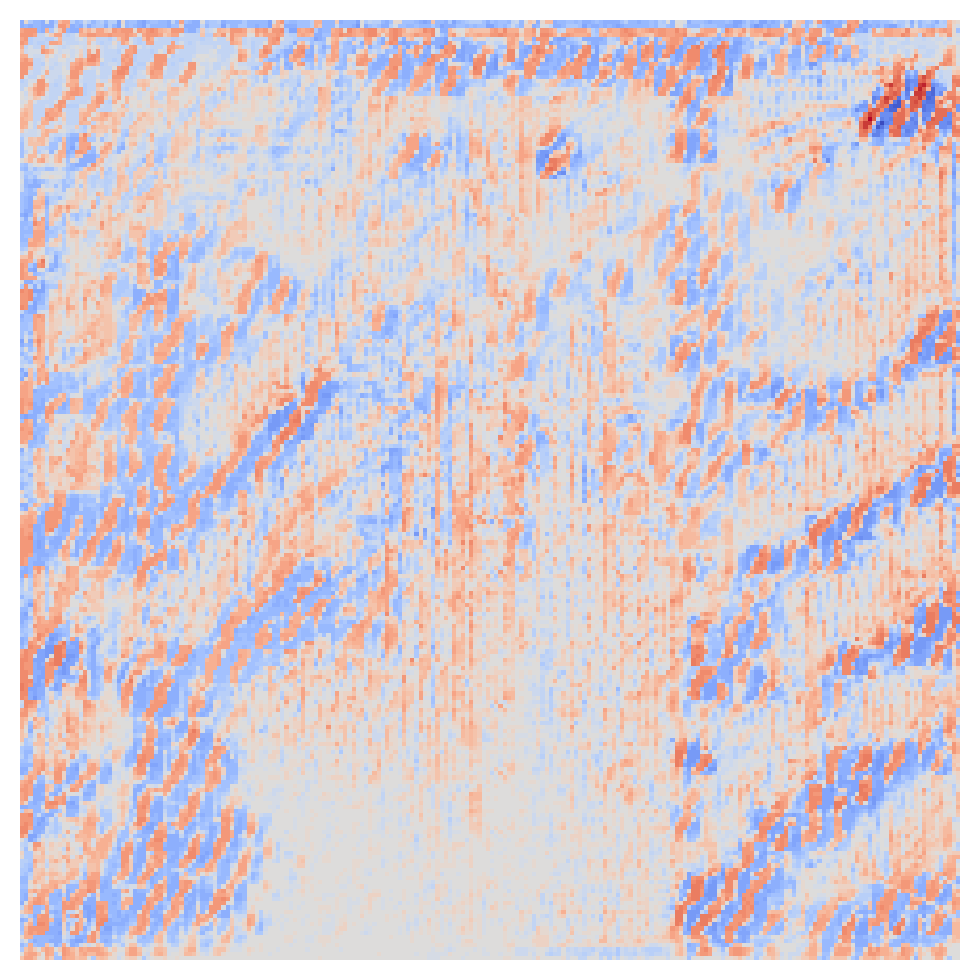
\includegraphics[height=1\linewidth]{01-images/05-resultate/uap_resnet/uap3-resnet18-covid-n200-robustificationslevel0.png}
        \caption{UAP Index 3}
    \end{subfigure}\hfill%
    \begin{subfigure}{0.19\linewidth}
        \centering
        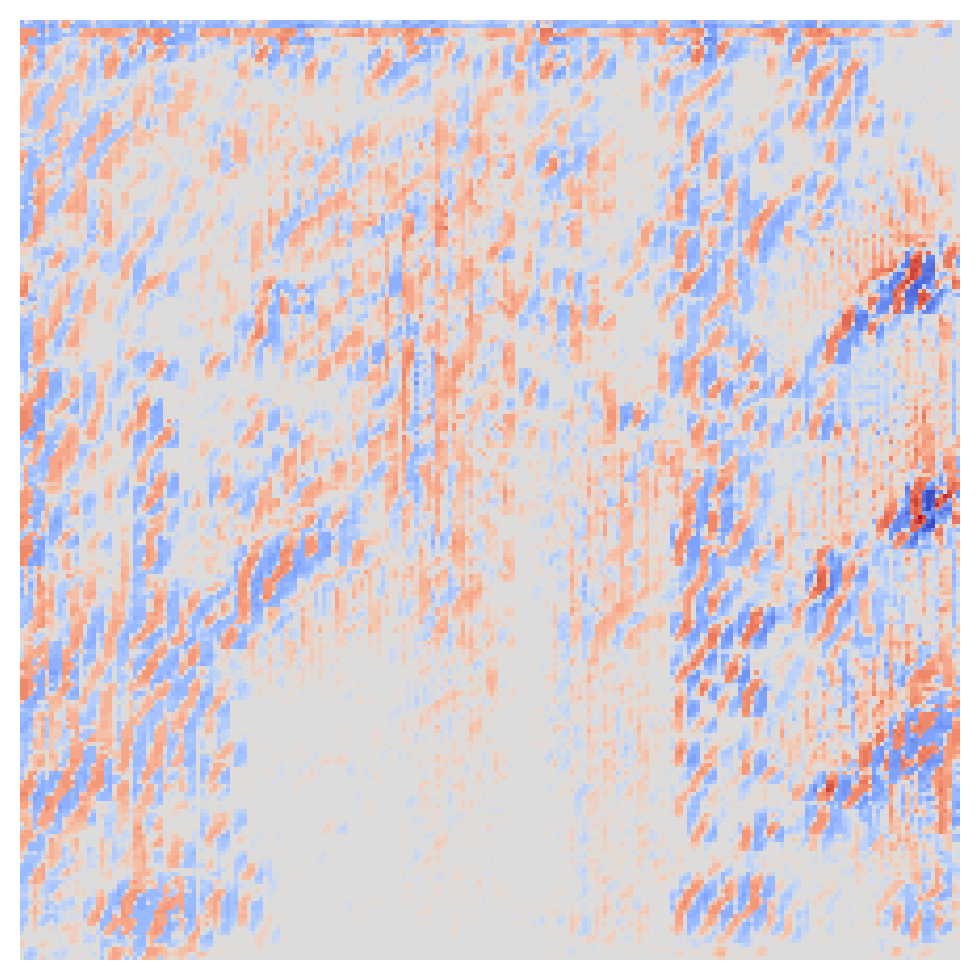
\includegraphics[height=1\linewidth]{01-images/05-resultate/uap_resnet/uap4-resnet18-covid-n200-robustificationslevel0.png}
        \caption{UAP Index 4}
    \end{subfigure}
    \caption{5 generierte UAPs durch 200 Trainingsbilder des mit ResNet18 trainierten Covidx Datensatzes vor der Robustifizierung durch adversarielles Training}
    \label{fig:uap-resnet18-covidx-rob0}
\end{figure}

in Abbildung \ref{} sind 5 UAPs vor der Robustifikation auf den Covidx Datensatz zu erkennen. 

% UAPs Resnet18 MRI robustifikations level 0
\begin{figure}[ht!]
    \centering
    \begin{subfigure}{0.19\linewidth}
        \centering
        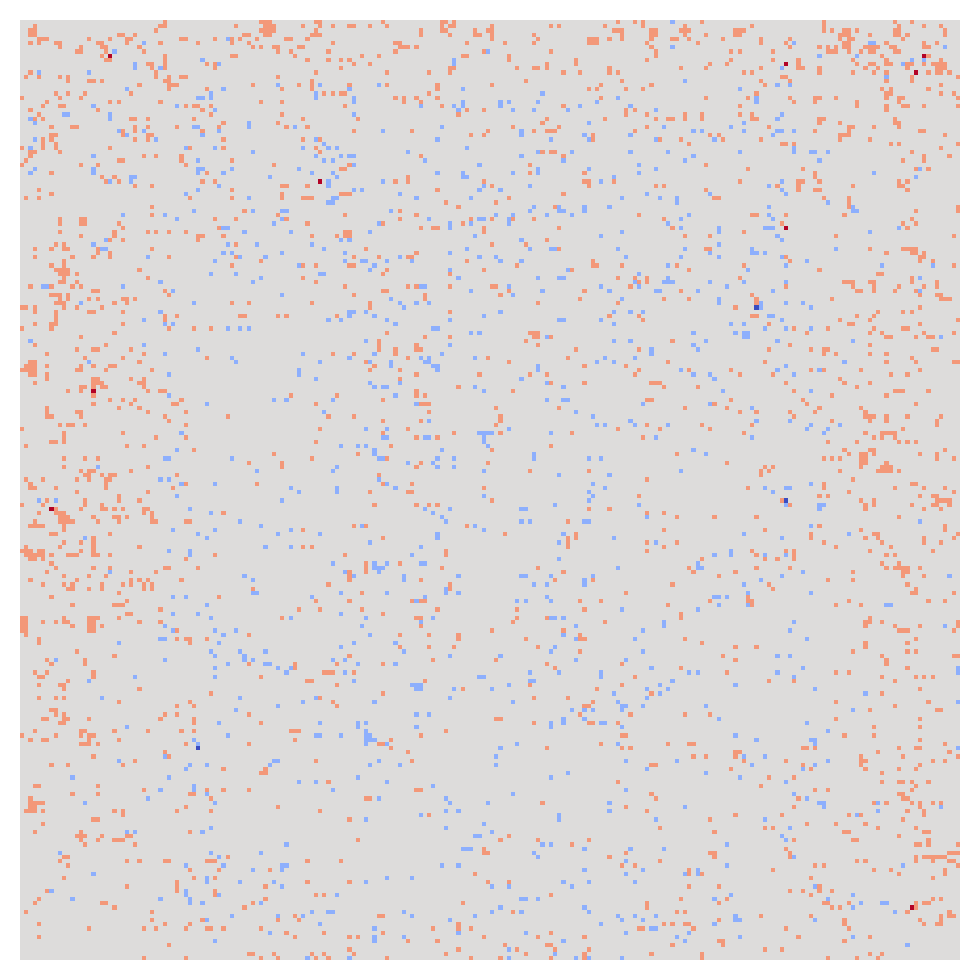
\includegraphics[height=1\linewidth]{01-images/05-resultate/uap_resnet/uap0-resnet18-mri-n200-robustificationslevel0.png}
        \caption{UAP Index 0}
    \end{subfigure}\hfill%
    \begin{subfigure}{0.19\linewidth}
        \centering
        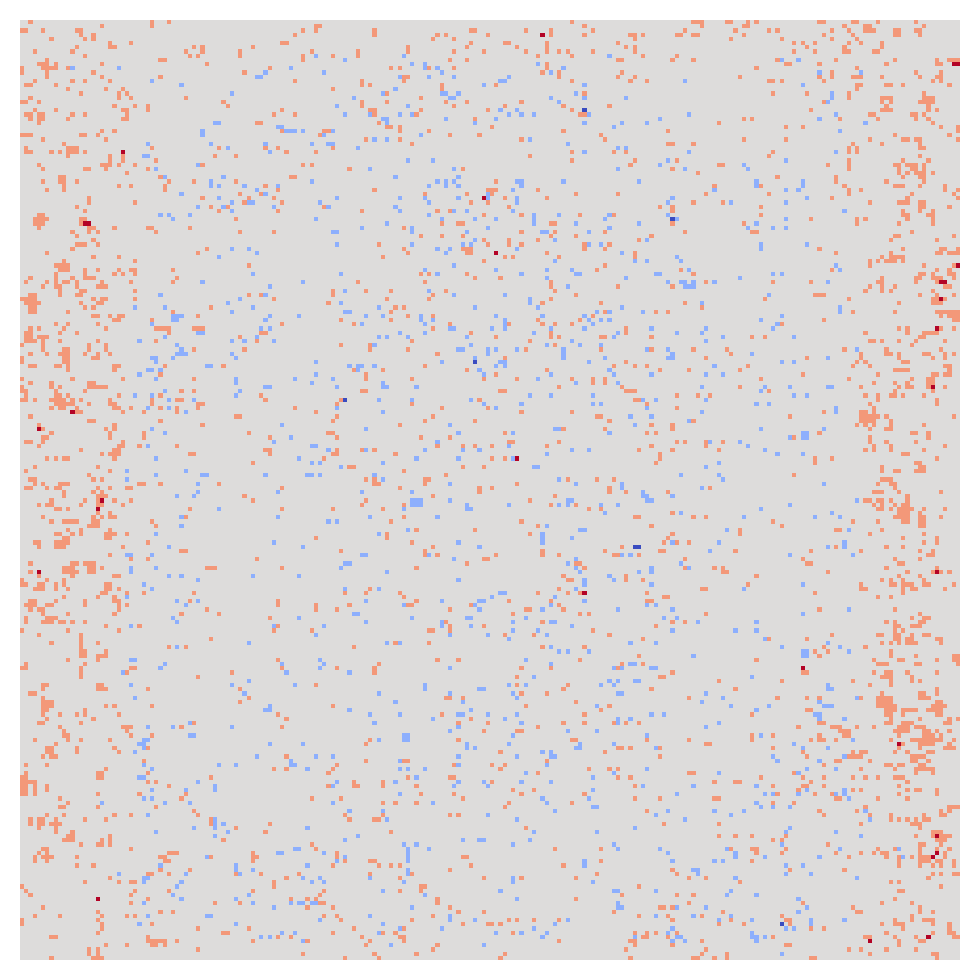
\includegraphics[height=1\linewidth]{01-images/05-resultate/uap_resnet/uap1-resnet18-mri-n200-robustificationslevel0.png}
        \caption{UAP Index 1}
    \end{subfigure}\hfill%
    \begin{subfigure}{0.19\linewidth}
        \centering
        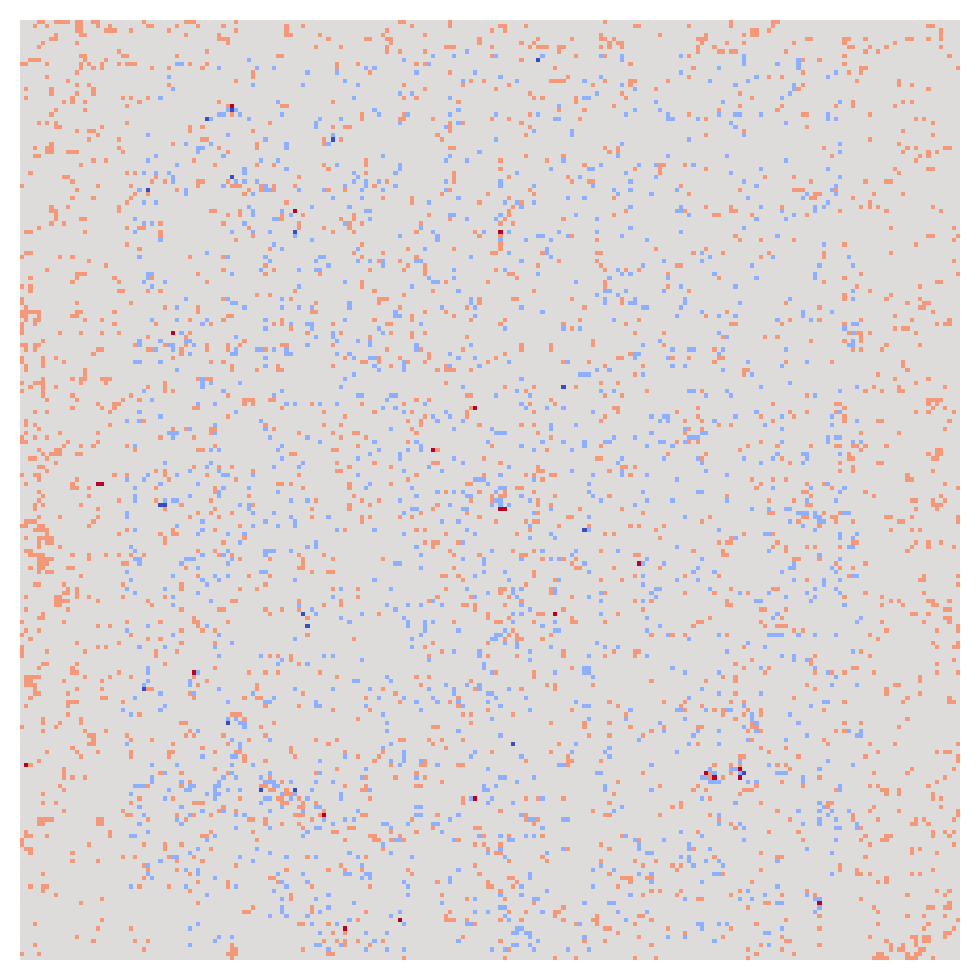
\includegraphics[height=1\linewidth]{01-images/05-resultate/uap_resnet/uap2-resnet18-mri-n200-robustificationslevel0.png}
        \caption{UAP Index 2}
    \end{subfigure}\hfill%
    \begin{subfigure}{0.19\linewidth}
        \centering
        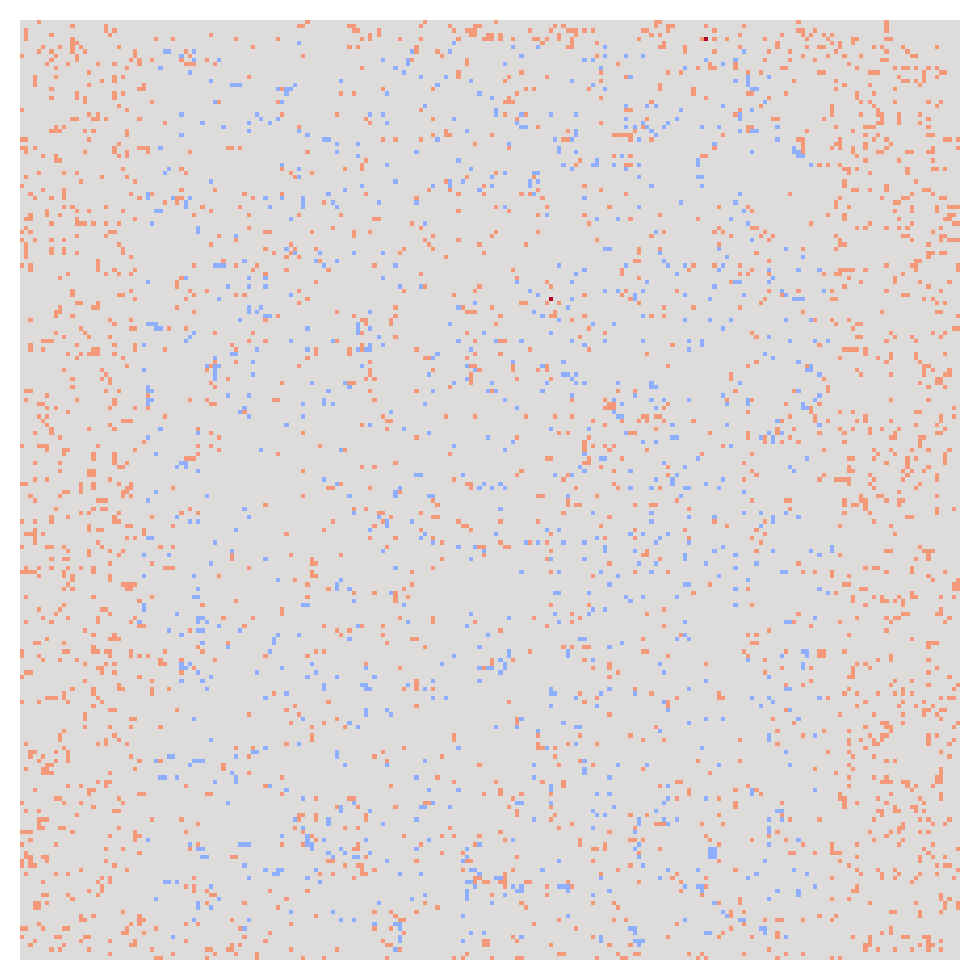
\includegraphics[height=1\linewidth]{01-images/05-resultate/uap_resnet/uap3-resnet18-mri-n200-robustificationslevel0.png}
        \caption{UAP Index 3}
    \end{subfigure}\hfill%
    \begin{subfigure}{0.19\linewidth}
        \centering
        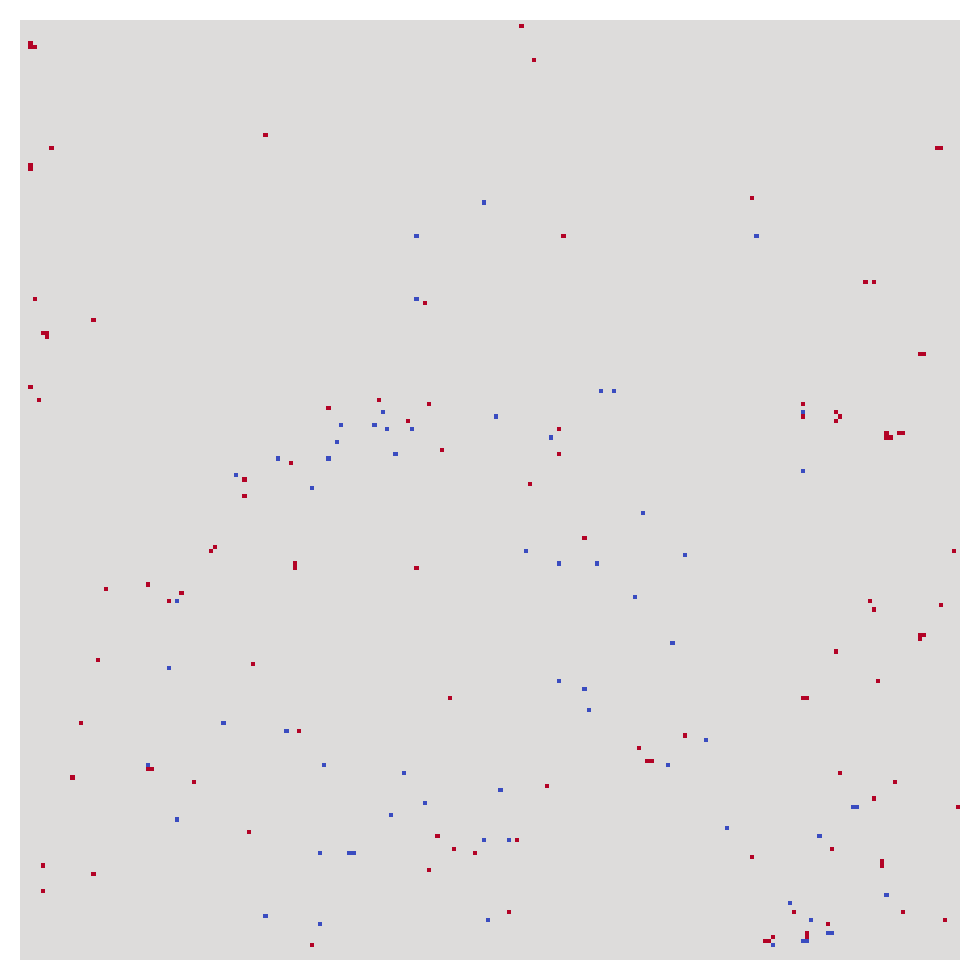
\includegraphics[height=1\linewidth]{01-images/05-resultate/uap_resnet/uap4-resnet18-mri-n200-robustificationslevel0.png}
        \caption{UAP Index 4}
    \end{subfigure}
    \caption{5 generierte UAPs durch 200 Trainingsbilder des mit ResNet18 trainierten Hirntumor Datensatzes vor der Robustifizierung durch adversarielles Training}
    \label{fig:uap-resnet18-mri-rob0}
\end{figure}

in Abbildung \ref{} sind 5 UAPs vor der Robustifikation auf den Hinrtumor Datensatz zu erkennen. 

\newpage

% UAP Vor und Nach Robustifikation
\begin{figure}[ht!]
    \centering
    \begin{subfigure}{0.19\linewidth}
        \centering
        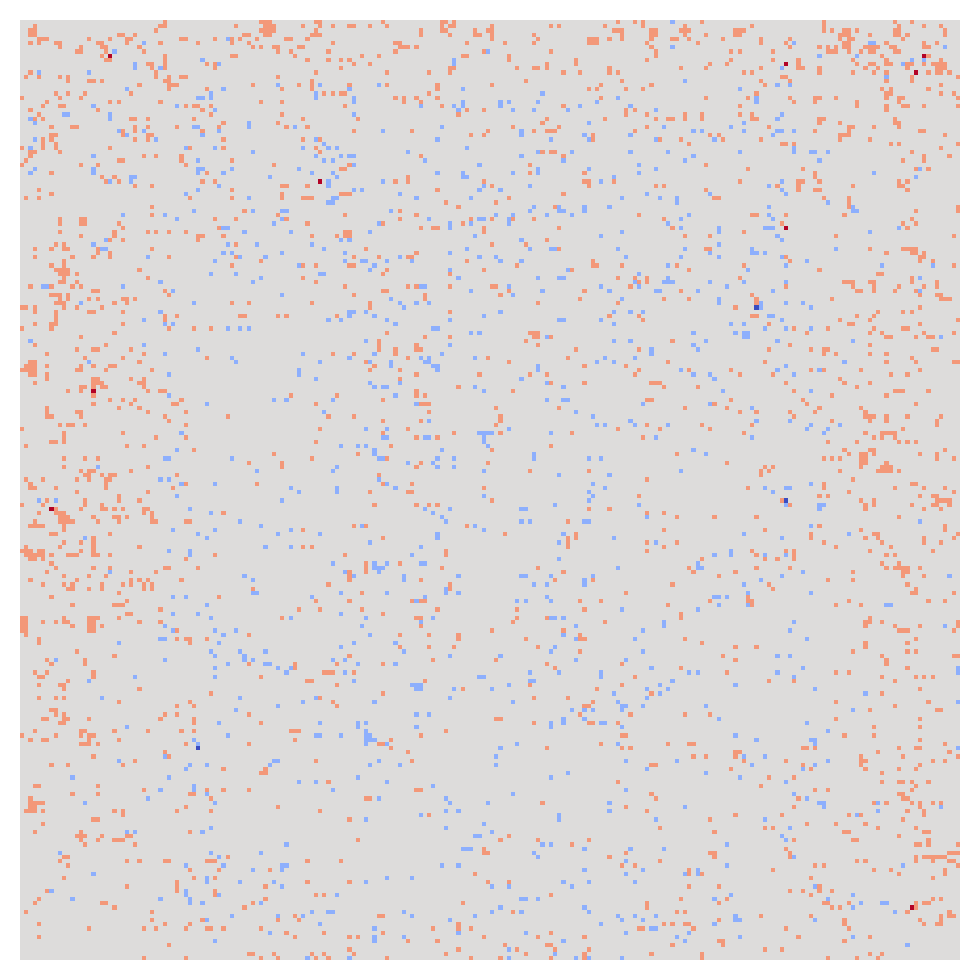
\includegraphics[height=1\linewidth]{01-images/05-resultate/uap_resnet/uap0-resnet18-mri-n200-robustificationslevel0.png}
        \caption{UAP 1 vor der Robustifikation}
    \end{subfigure}
    \begin{subfigure}{0.19\linewidth}
        \centering
        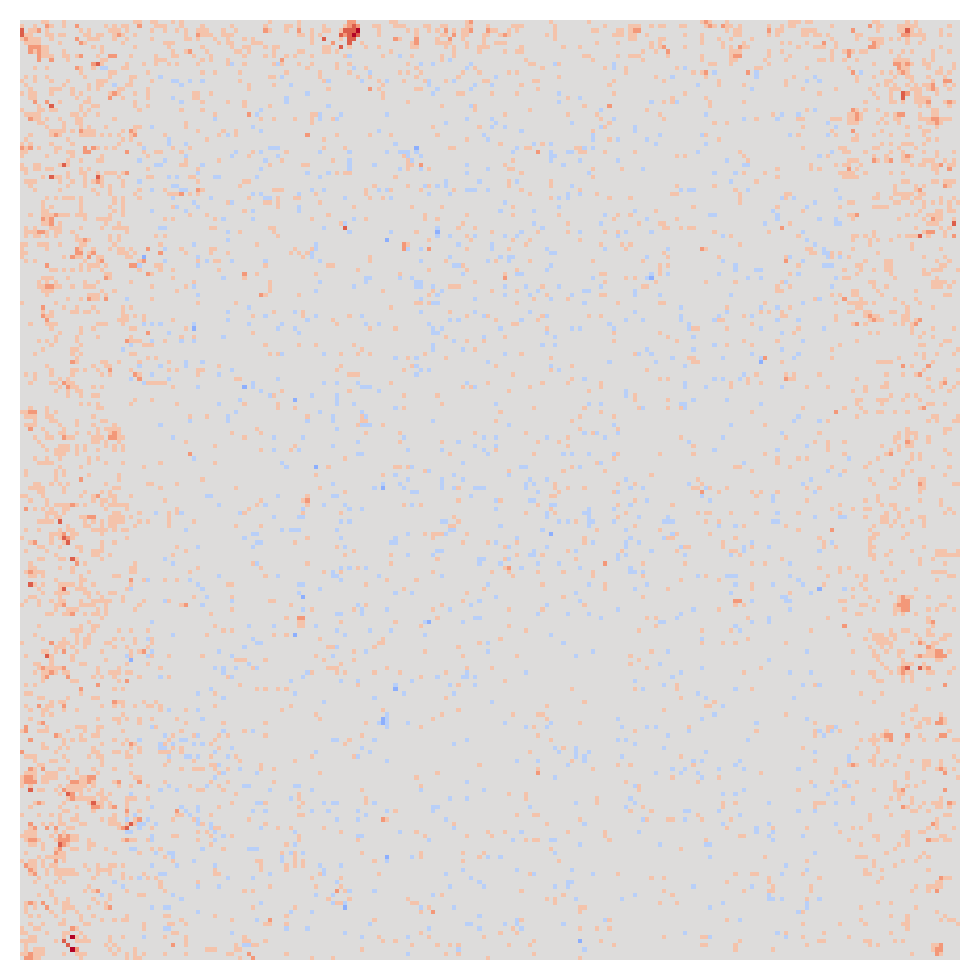
\includegraphics[height=1\linewidth]{01-images/05-resultate/uap_resnet/uap0-resnet18-mri-n200-robustificationslevel7.png}
        \caption{UAP 1 nach der Robustifikation}
    \end{subfigure}
    \hfill%
    \begin{subfigure}{0.19\linewidth}
        \centering
        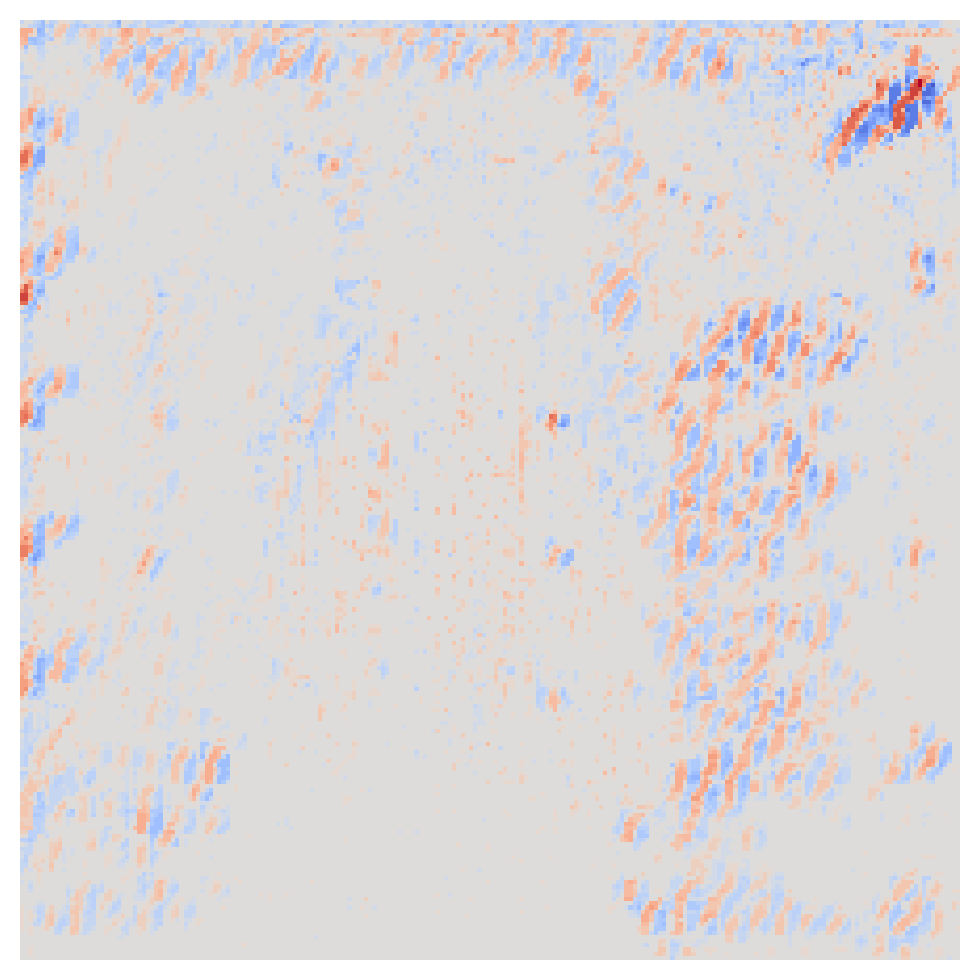
\includegraphics[height=1\linewidth]{01-images/05-resultate/uap_resnet/uap0-resnet18-covid-n200-robustificationslevel0.png}
        \caption{UAP 1 vor der Robustifikation}
    \end{subfigure}
    \begin{subfigure}{0.19\linewidth}
        \centering
        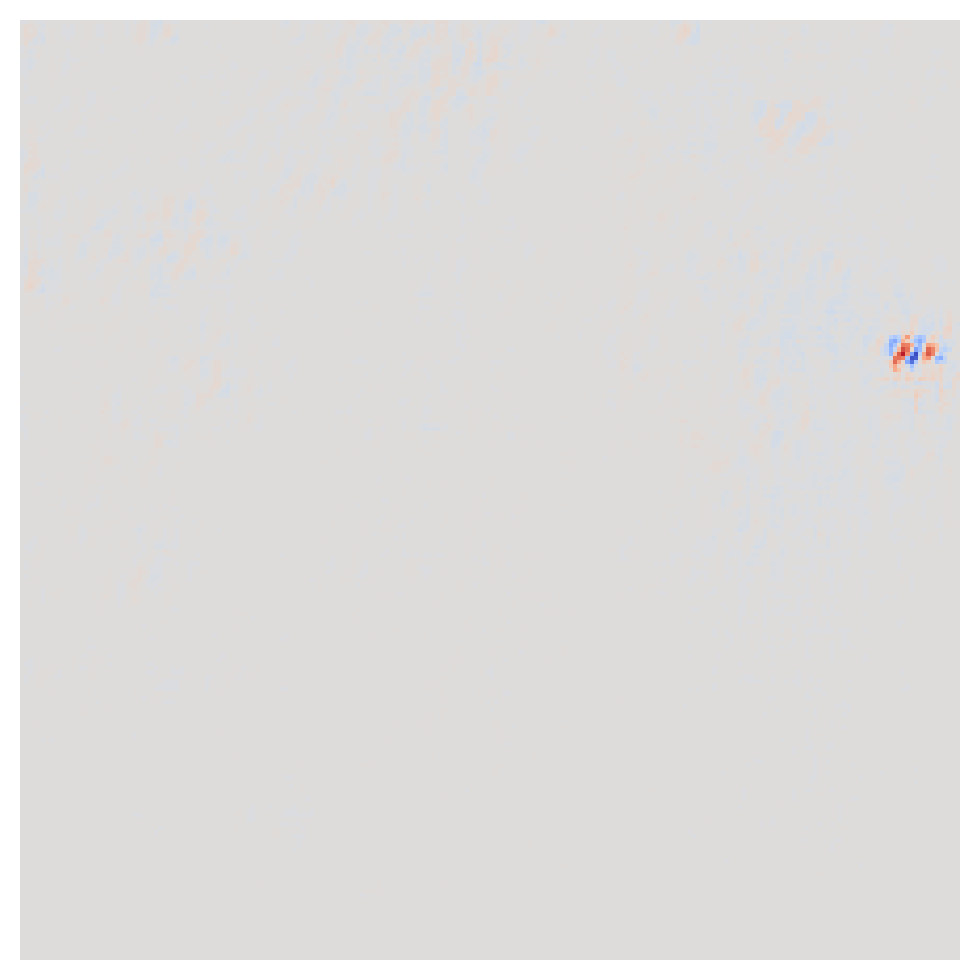
\includegraphics[height=1\linewidth]{01-images/05-resultate/uap_resnet/uap0-resnet18-covid-n200-robustificationslevel7.png}
        \caption{UAP 1 nach der Robustifikation}
    \end{subfigure}
    \caption{Generierte UAP vor und nach der Robustifikation für Covid und Hirntumor Datensatz}
    \label{fig:uap-resnet18-mri-rob0}
\end{figure}

Ein Vergleich von vor und nach der robustifikation ist in Abbildung \ref{} zu sehen

% UAP Robustifikationslevel
\begin{figure}[ht!]
    \centering
    \begin{subfigure}{0.095\linewidth}
        \centering
        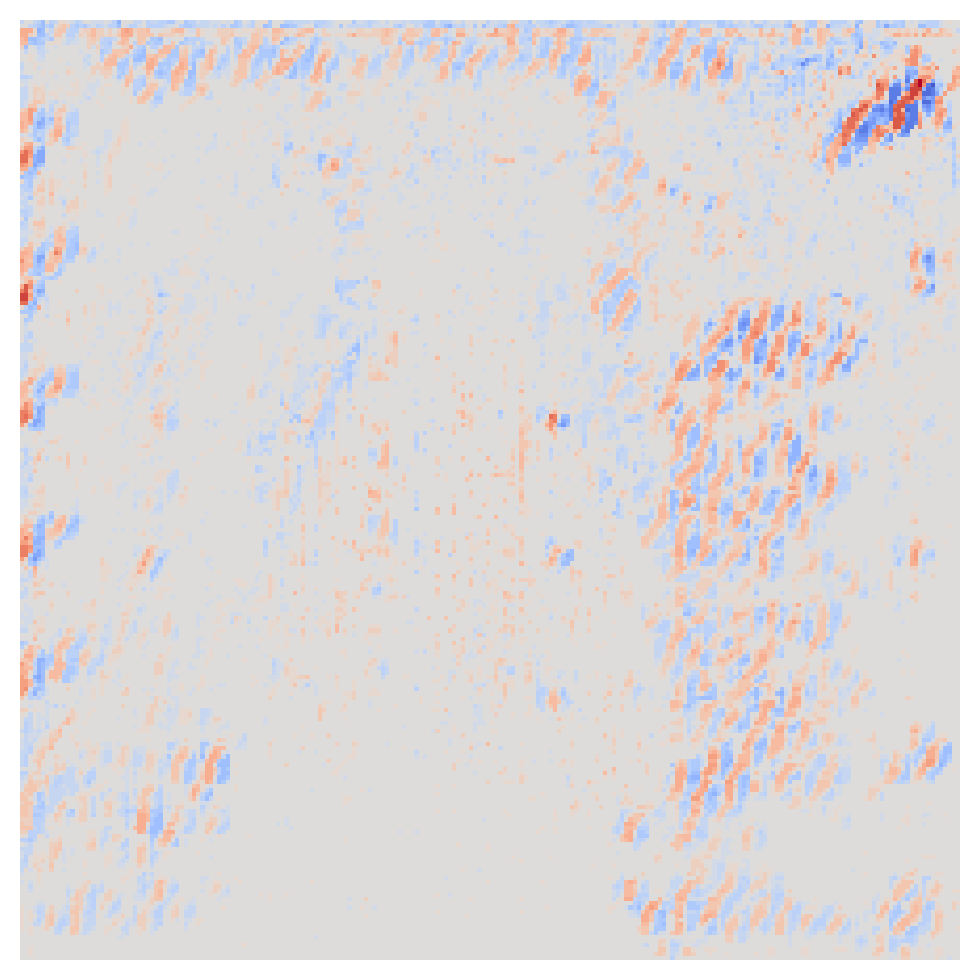
\includegraphics[height=1\linewidth]{01-images/05-resultate/uap_resnet/uap0-resnet18-covid-n200-robustificationslevel0.png}
        \caption{0}
    \end{subfigure}\hfill%
    \begin{subfigure}{0.095\linewidth}
        \centering
        
\includegraphics[height=1\linewidth]{01-images/05-resultate/uap_resnet/uap0-resnet18-covid-n200-robustificationslevel1.png}
        \caption{1}
    \end{subfigure}\hfill%
    \begin{subfigure}{0.095\linewidth}
        \centering
        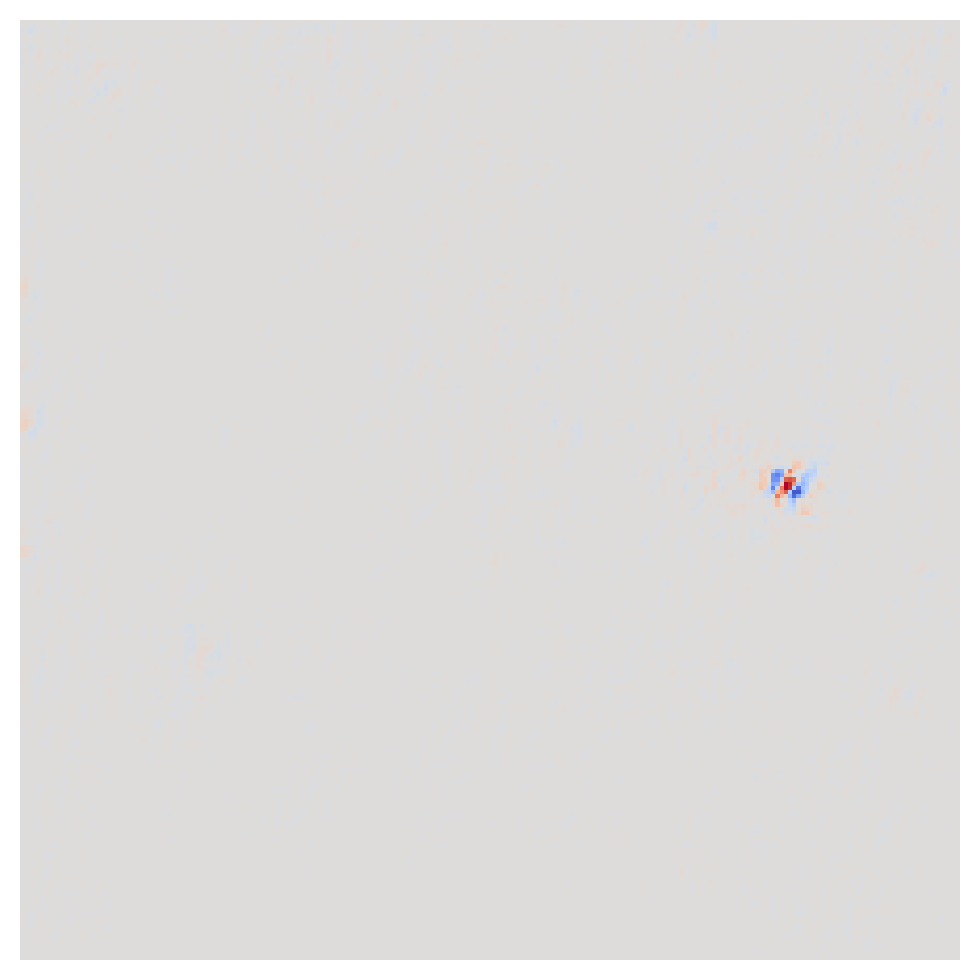
\includegraphics[height=1\linewidth]{01-images/05-resultate/uap_resnet/uap0-resnet18-covid-n200-robustificationslevel2.png}
        \caption{2}
    \end{subfigure}\hfill%
    \begin{subfigure}{0.095\linewidth}
        \centering
        
\includegraphics[height=1\linewidth]{01-images/05-resultate/uap_resnet/uap0-resnet18-covid-n200-robustificationslevel3.png}
        \caption{3}
    \end{subfigure}\hfill%
    \begin{subfigure}{0.095\linewidth}
        \centering
        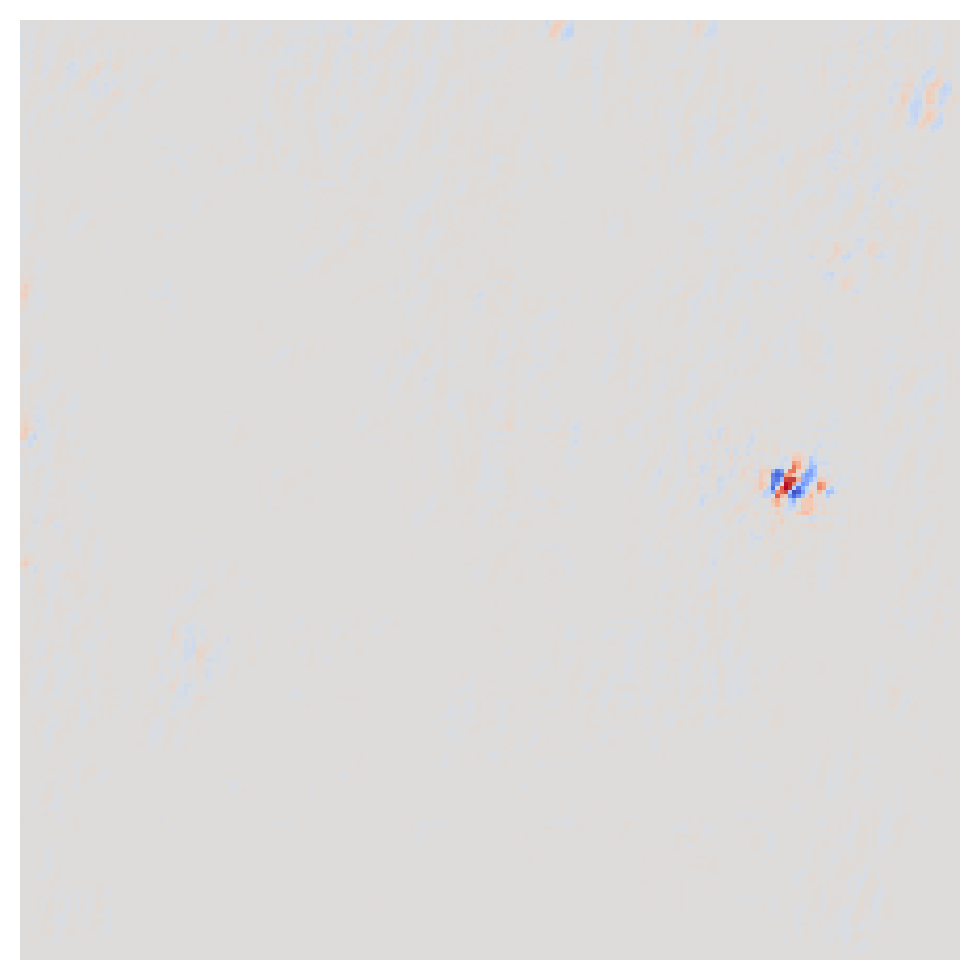
\includegraphics[height=1\linewidth]{01-images/05-resultate/uap_resnet/uap0-resnet18-covid-n200-robustificationslevel4.png}
        \caption{4}
    \end{subfigure}\hfill%
    \begin{subfigure}{0.095\linewidth}
        \centering
        
\includegraphics[height=1\linewidth]{01-images/05-resultate/uap_resnet/uap0-resnet18-covid-n200-robustificationslevel5.png}
        \caption{5}
    \end{subfigure}\hfill%
    \begin{subfigure}{0.095\linewidth}
        \centering
        
\includegraphics[height=1\linewidth]{01-images/05-resultate/uap_resnet/uap0-resnet18-covid-n200-robustificationslevel6.png}
        \caption{6}
    \end{subfigure}\hfill%
    \begin{subfigure}{0.095\linewidth}
        \centering
        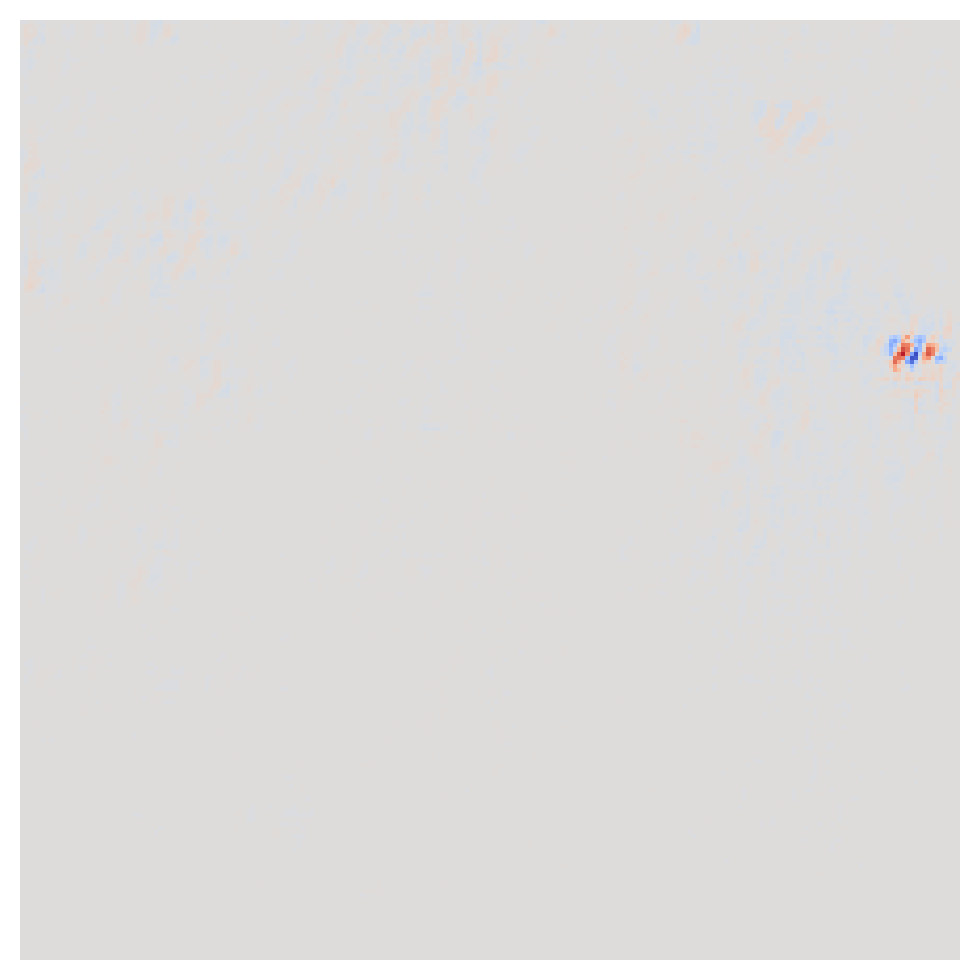
\includegraphics[height=1\linewidth]{01-images/05-resultate/uap_resnet/uap0-resnet18-covid-n200-robustificationslevel7.png}
        \caption{7}
    \end{subfigure}\hfill%
    \begin{subfigure}{0.095\linewidth}
        \centering
        
\includegraphics[height=1\linewidth]{01-images/05-resultate/uap_resnet/uap0-resnet18-covid-n200-robustificationslevel8.png}
        \caption{8}
    \end{subfigure}\hfill%
    \begin{subfigure}{0.095\linewidth}
        \centering
        
\includegraphics[height=1\linewidth]{01-images/05-resultate/uap_resnet/uap0-resnet18-covid-n200-robustificationslevel9.png}
        \caption{9}
    \end{subfigure}
    \caption{Generierte UAPs durch 200 Trainigsbilder des mit ResNet18 trainierten Hirntumor Datensatzes nach jeder Robustifikationslevel druch adversarial Training von links nach rechts}
    \label{fig:uap-resnet18-covidx-rob0}
\end{figure}

Hier in dieser Abbildung \ref{} sind jeweils nur die UAP Index 0 zu erkennen durch unterschiedliche Robustifikationslevel zu erkennen. 

\begin{figure}[ht!]
    \centering
    \begin{subfigure}{0.095\linewidth}
        \centering
        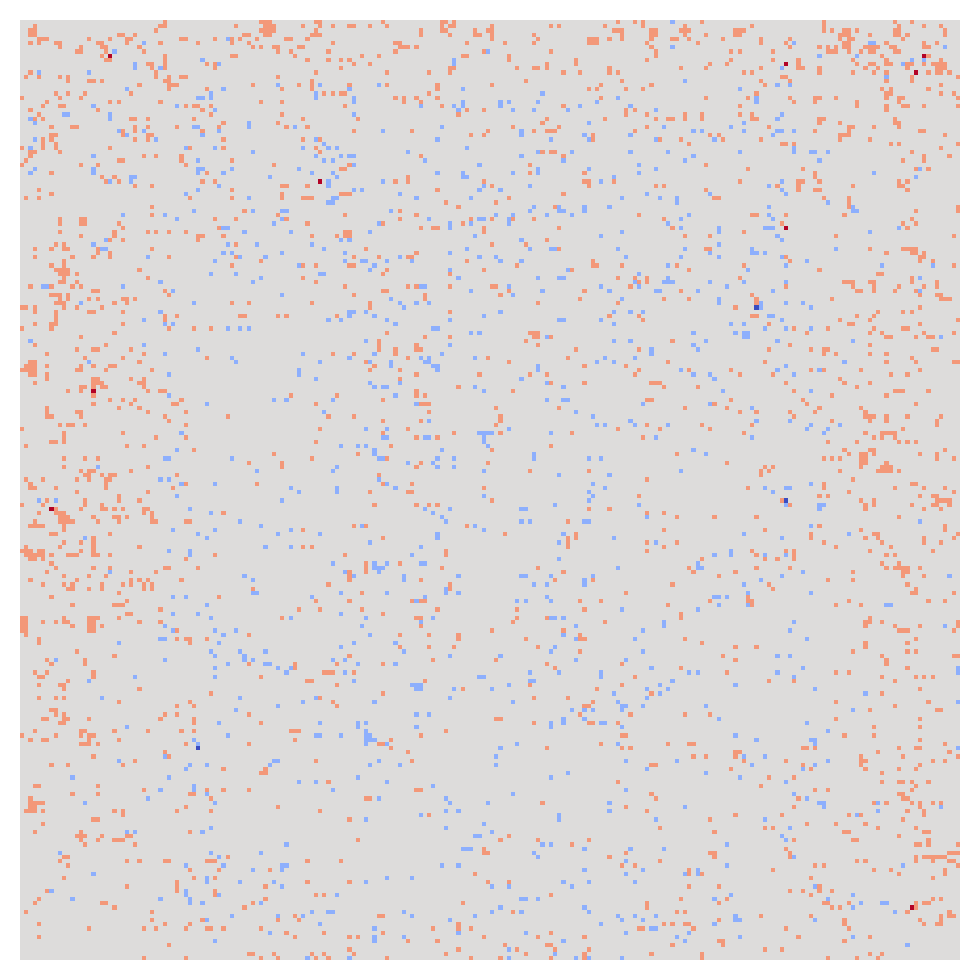
\includegraphics[height=1\linewidth]{01-images/05-resultate/uap_resnet/uap0-resnet18-mri-n200-robustificationslevel0.png}
        \caption{0}
    \end{subfigure}\hfill%
    \begin{subfigure}{0.095\linewidth}
        \centering
        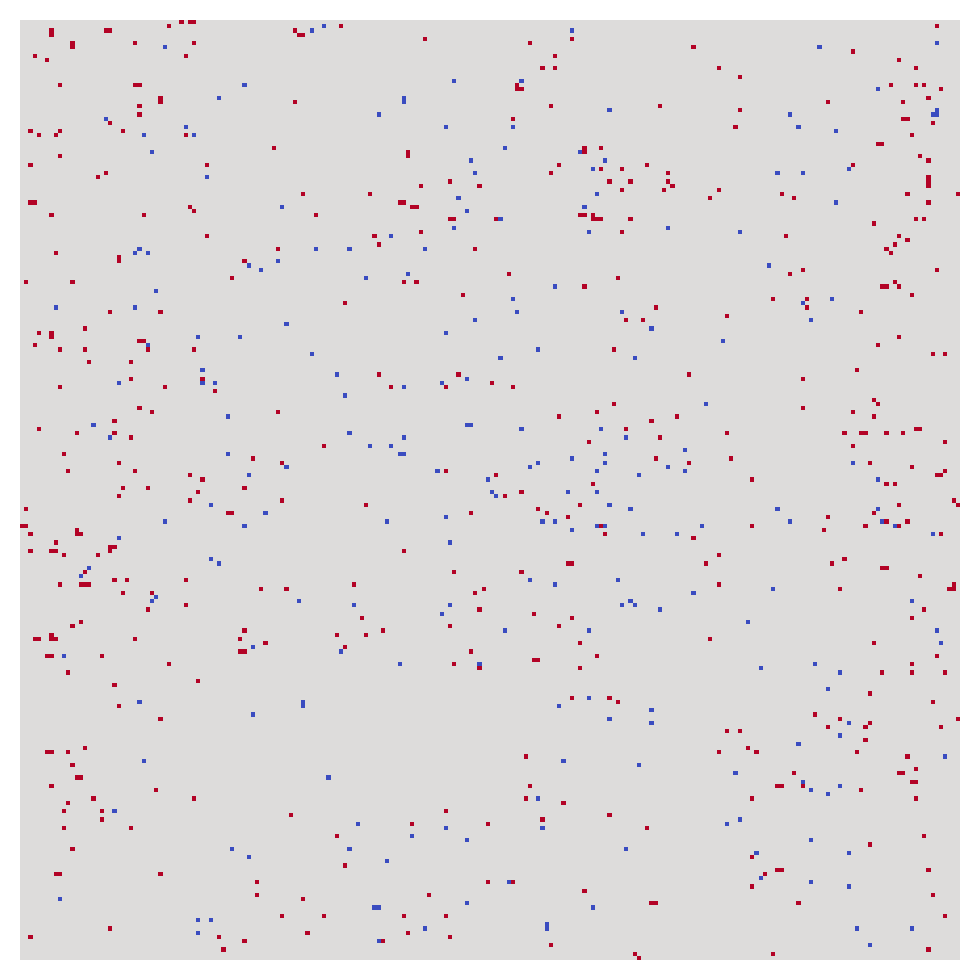
\includegraphics[height=1\linewidth]{01-images/05-resultate/uap_resnet/uap0-resnet18-mri-n200-robustificationslevel1.png}
        \caption{1}
    \end{subfigure}\hfill%
    \begin{subfigure}{0.095\linewidth}
        \centering
        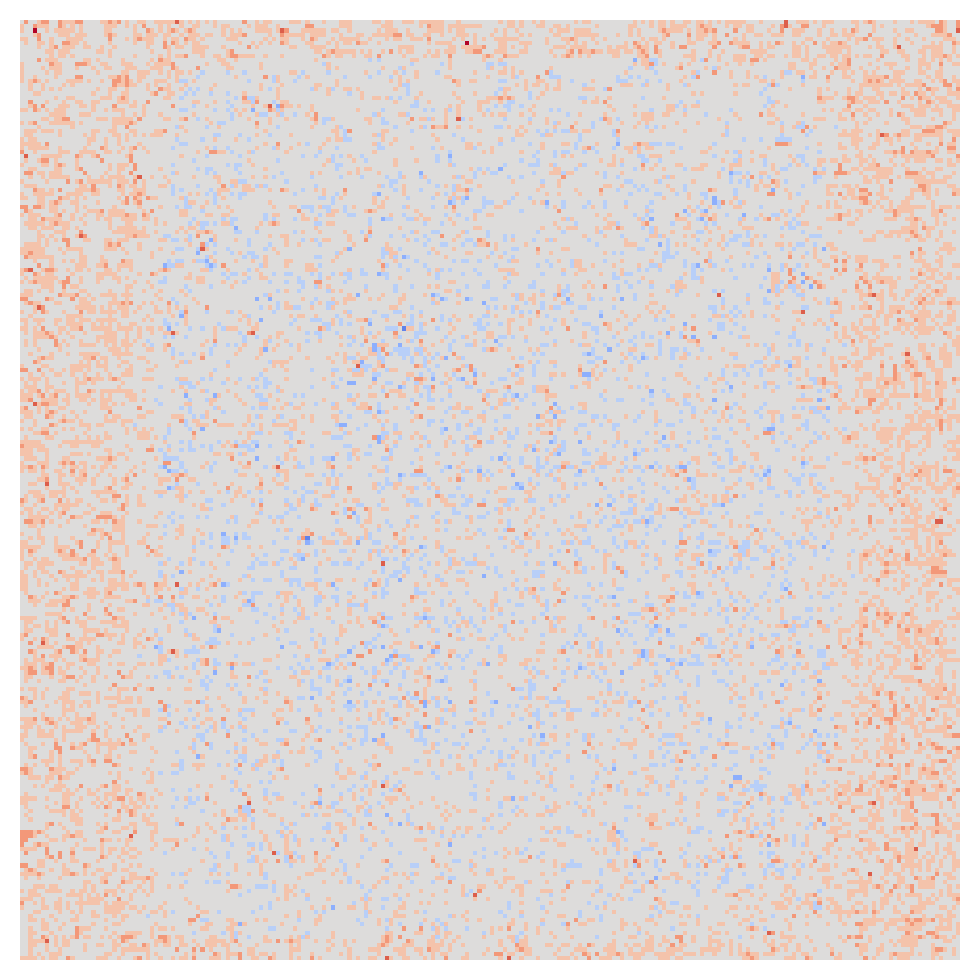
\includegraphics[height=1\linewidth]{01-images/05-resultate/uap_resnet/uap0-resnet18-mri-n200-robustificationslevel2.png}
        \caption{2}
    \end{subfigure}\hfill%
    \begin{subfigure}{0.095\linewidth}
        \centering
        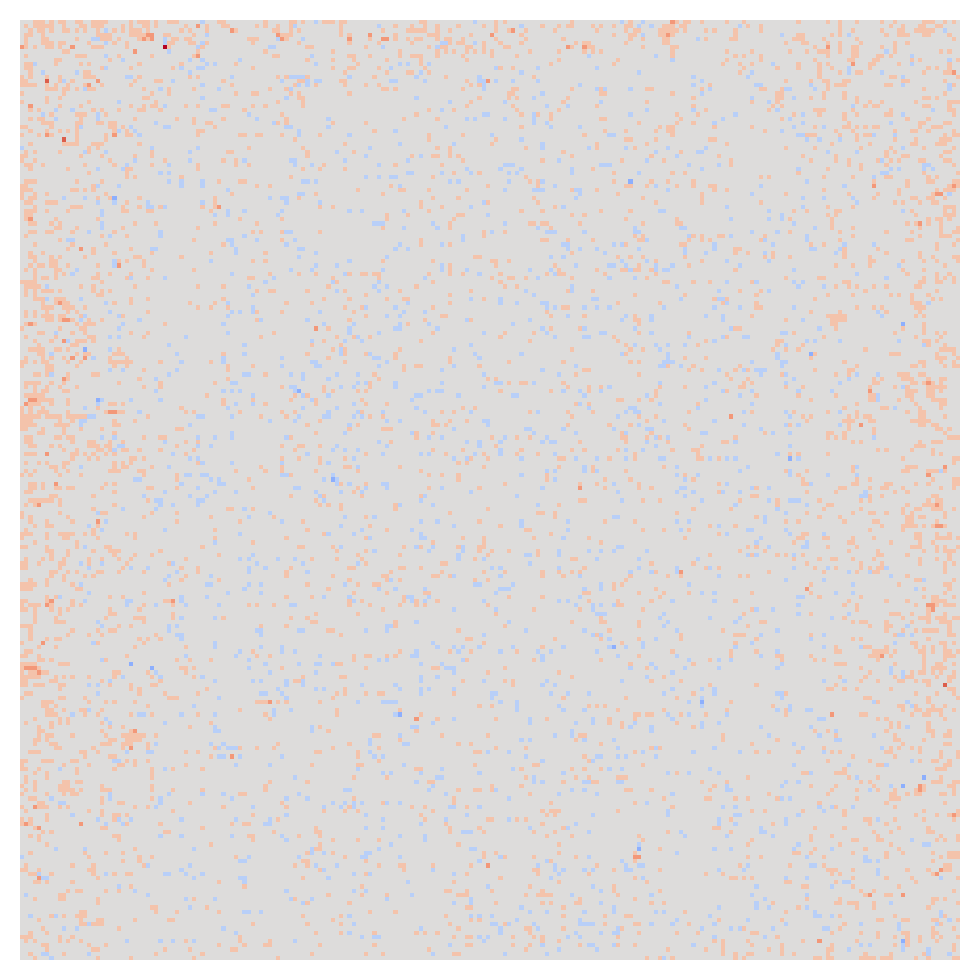
\includegraphics[height=1\linewidth]{01-images/05-resultate/uap_resnet/uap0-resnet18-mri-n200-robustificationslevel3.png}
        \caption{3}
    \end{subfigure}\hfill%
    \begin{subfigure}{0.095\linewidth}
        \centering
        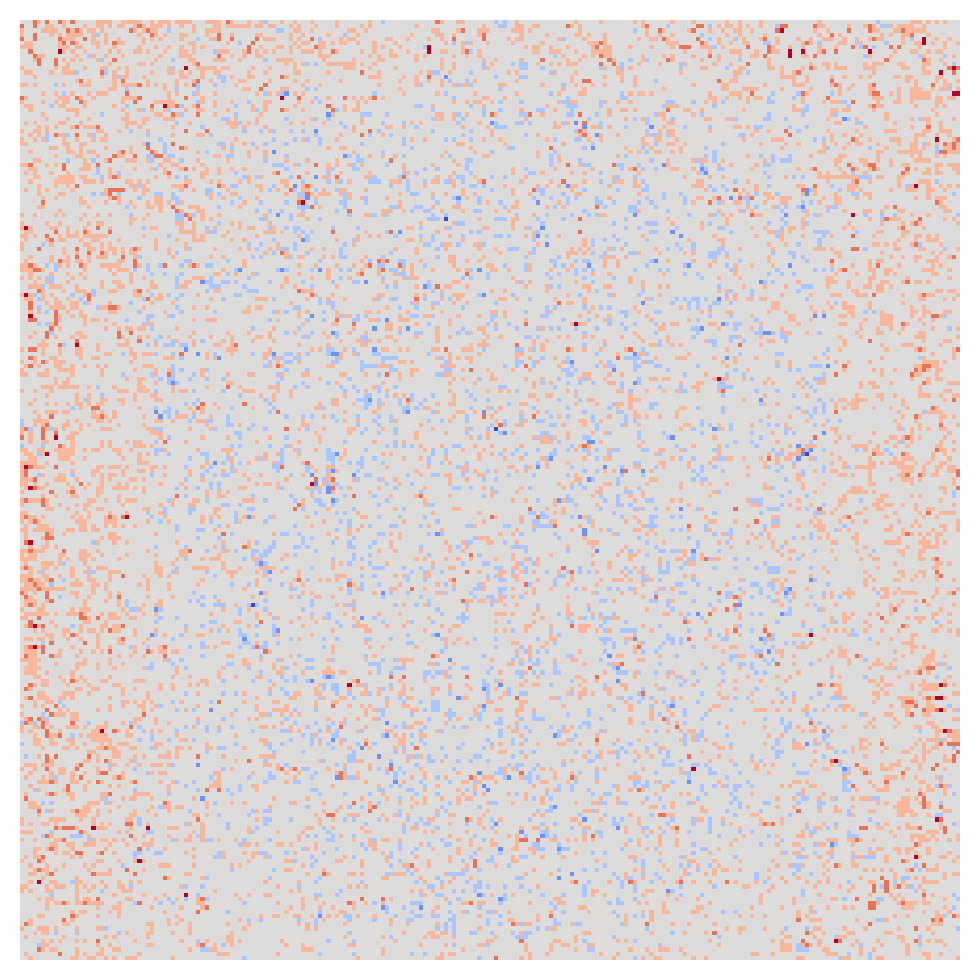
\includegraphics[height=1\linewidth]{01-images/05-resultate/uap_resnet/uap0-resnet18-mri-n200-robustificationslevel4.png}
        \caption{4}
    \end{subfigure}\hfill%
    \begin{subfigure}{0.095\linewidth}
        \centering
        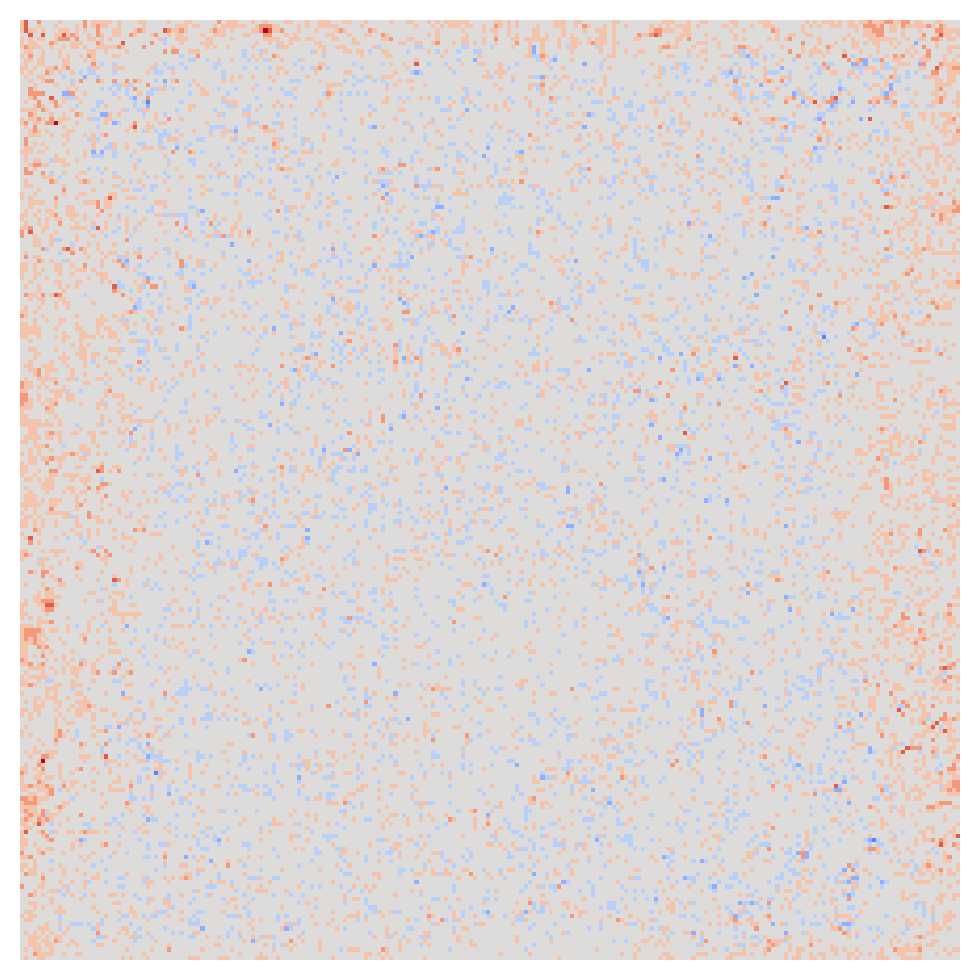
\includegraphics[height=1\linewidth]{01-images/05-resultate/uap_resnet/uap0-resnet18-mri-n200-robustificationslevel5.png}
        \caption{5}
    \end{subfigure}\hfill%
    \begin{subfigure}{0.095\linewidth}
        \centering
        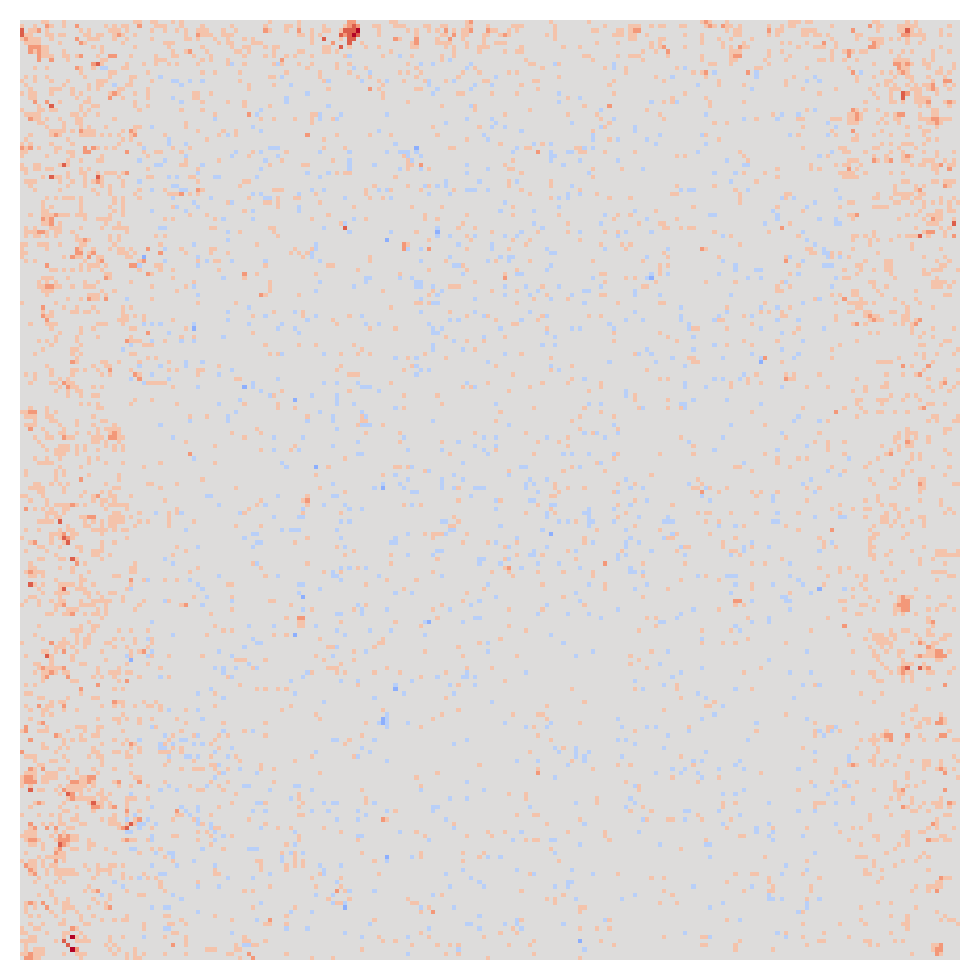
\includegraphics[height=1\linewidth]{01-images/05-resultate/uap_resnet/uap0-resnet18-mri-n200-robustificationslevel6.png}
        \caption{6}
    \end{subfigure}
    \caption{Generierte UAPs durch 200 Trainigsbilder des mit ResNet18 trainierten Hirntumor Datensatzes nach jeder Robustifikationslevel druch adversarial Training von links nach rechts}
    \label{fig:uap-resnet18-covidx-rob0}
\end{figure}




\subsubsection{UAP ResNet50}
\todo{Kapitel noch in Arbeit}
In diesem Kapitel visualisieren wir die UAP, welches durch das ResNet18 Modell erstellt wurden.

% UAPs Resnet18 covidx robustifikations level 0
\begin{figure}[ht!]
    \centering
    \begin{subfigure}{0.19\linewidth}
        \centering
        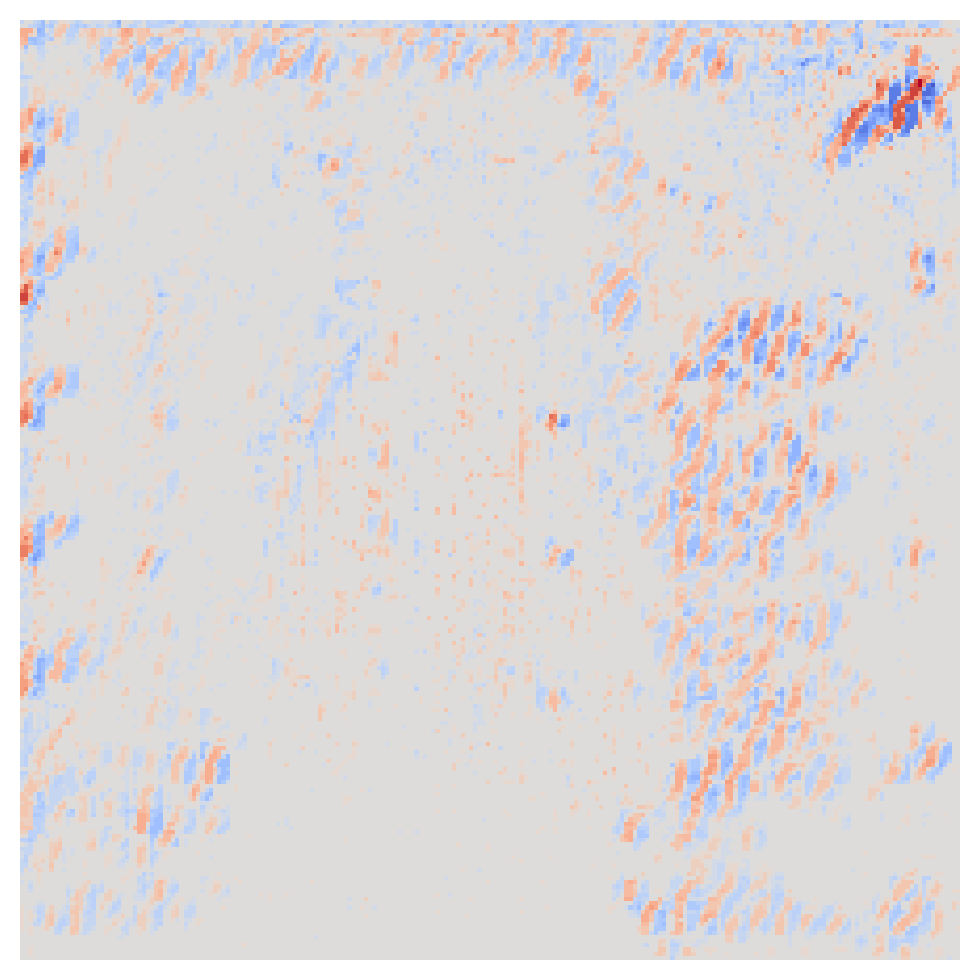
\includegraphics[height=1\linewidth]{01-images/05-resultate/uap_resnet/uap0-resnet18-covid-n200-robustificationslevel0.png}
        \caption{UAP Index 0}
    \end{subfigure}\hfill%
    \begin{subfigure}{0.19\linewidth}
        \centering
        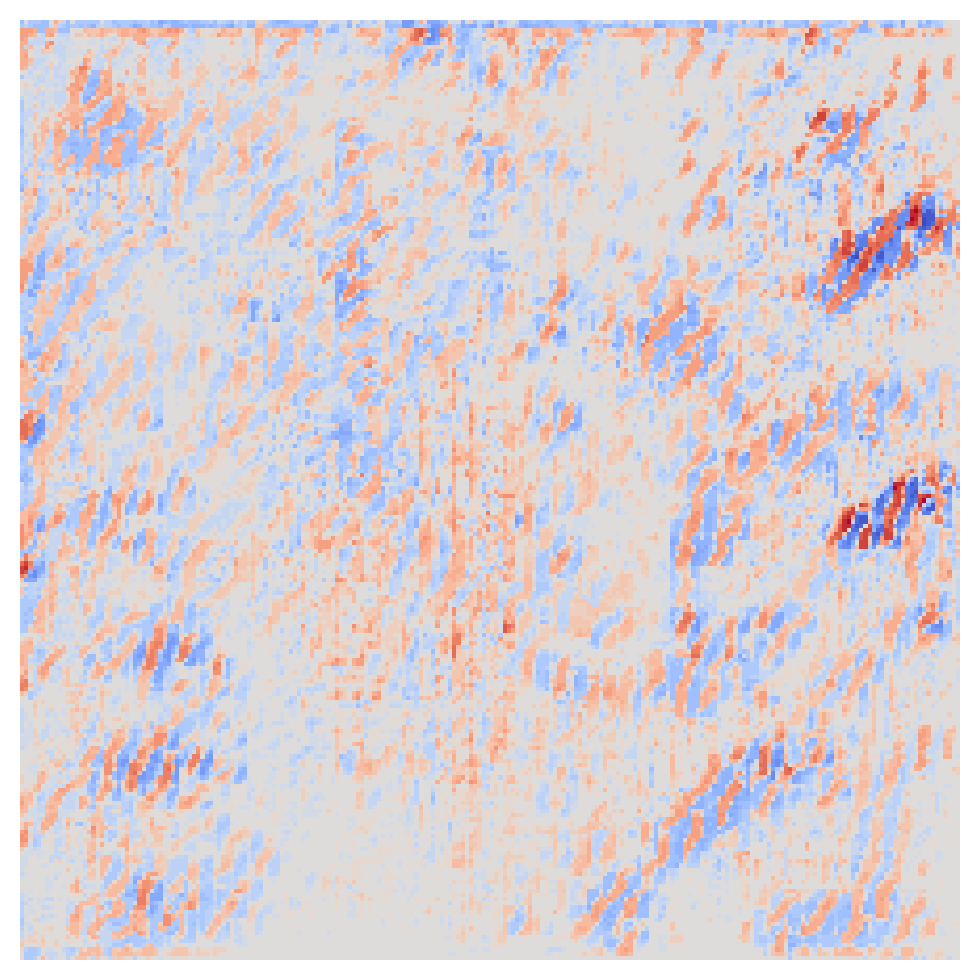
\includegraphics[height=1\linewidth]{01-images/05-resultate/uap_resnet/uap1-resnet18-covid-n200-robustificationslevel0.png}
        \caption{UAP Index 1}
    \end{subfigure}\hfill%
    \begin{subfigure}{0.19\linewidth}
        \centering
        \includegraphics[height=1\linewidth]{01-images/05-resultate/uap_resnet/uap2-resnet18-covid-n200-robustificationslevel0.png}
        \caption{UAP Index 2}
    \end{subfigure}\hfill%
    \begin{subfigure}{0.19\linewidth}
        \centering
        \includegraphics[height=1\linewidth]{01-images/05-resultate/uap_resnet/uap3-resnet18-covid-n200-robustificationslevel0.png}
        \caption{UAP Index 3}
    \end{subfigure}\hfill%
    \begin{subfigure}{0.19\linewidth}
        \centering
        \includegraphics[height=1\linewidth]{01-images/05-resultate/uap_resnet/uap4-resnet18-covid-n200-robustificationslevel0.png}
        \caption{UAP Index 4}
    \end{subfigure}
    \caption{5 generierte UAPs durch 200 Trainingsbilder des mit ResNet18 trainierten Covidx Datensatzes vor der Robustifizierung durch adversarielles Training}
    \label{fig:uap-resnet18-covidx-rob0}
\end{figure}

in Abbildung \ref{} sind 5 UAPs vor der Robustifikation auf den Covidx Datensatz zu erkennen. 

% UAPs Resnet18 MRI robustifikations level 0
\begin{figure}[ht!]
    \centering
    \begin{subfigure}{0.19\linewidth}
        \centering
        \includegraphics[height=1\linewidth]{01-images/05-resultate/uap_resnet/uap0-resnet18-mri-n200-robustificationslevel0.png}
        \caption{UAP Index 0}
    \end{subfigure}\hfill%
    \begin{subfigure}{0.19\linewidth}
        \centering
        \includegraphics[height=1\linewidth]{01-images/05-resultate/uap_resnet/uap1-resnet18-mri-n200-robustificationslevel0.png}
        \caption{UAP Index 1}
    \end{subfigure}\hfill%
    \begin{subfigure}{0.19\linewidth}
        \centering
        \includegraphics[height=1\linewidth]{01-images/05-resultate/uap_resnet/uap2-resnet18-mri-n200-robustificationslevel0.png}
        \caption{UAP Index 2}
    \end{subfigure}\hfill%
    \begin{subfigure}{0.19\linewidth}
        \centering
        \includegraphics[height=1\linewidth]{01-images/05-resultate/uap_resnet/uap3-resnet18-mri-n200-robustificationslevel0.png}
        \caption{UAP Index 3}
    \end{subfigure}\hfill%
    \begin{subfigure}{0.19\linewidth}
        \centering
        \includegraphics[height=1\linewidth]{01-images/05-resultate/uap_resnet/uap4-resnet18-mri-n200-robustificationslevel0.png}
        \caption{UAP Index 4}
    \end{subfigure}
    \caption{5 generierte UAPs durch 200 Trainingsbilder des mit ResNet18 trainierten Hirntumor Datensatzes vor der Robustifizierung durch adversarielles Training}
    \label{fig:uap-resnet18-mri-rob0}
\end{figure}

in Abbildung \ref{} sind 5 UAPs vor der Robustifikation auf den Hinrtumor Datensatz zu erkennen. 

\newpage

% UAP Vor und Nach Robustifikation
\begin{figure}[ht!]
    \centering
    \begin{subfigure}{0.19\linewidth}
        \centering
        \includegraphics[height=1\linewidth]{01-images/05-resultate/uap_resnet/uap0-resnet18-mri-n200-robustificationslevel0.png}
        \caption{UAP 1 vor der Robustifikation}
    \end{subfigure}
    \begin{subfigure}{0.19\linewidth}
        \centering
        \includegraphics[height=1\linewidth]{01-images/05-resultate/uap_resnet/uap0-resnet18-mri-n200-robustificationslevel7.png}
        \caption{UAP 1 nach der Robustifikation}
    \end{subfigure}
    \hfill%
    \begin{subfigure}{0.19\linewidth}
        \centering
        \includegraphics[height=1\linewidth]{01-images/05-resultate/uap_resnet/uap0-resnet18-covid-n200-robustificationslevel0.png}
        \caption{UAP 1 vor der Robustifikation}
    \end{subfigure}
    \begin{subfigure}{0.19\linewidth}
        \centering
        \includegraphics[height=1\linewidth]{01-images/05-resultate/uap_resnet/uap0-resnet18-covid-n200-robustificationslevel7.png}
        \caption{UAP 1 nach der Robustifikation}
    \end{subfigure}
    \caption{Generierte UAP vor und nach der Robustifikation für Covid und Hirntumor Datensatz}
    \label{fig:uap-resnet18-mri-rob0}
\end{figure}

Ein Vergleich von vor und nach der robustifikation ist in Abbildung \ref{} zu sehen

% UAP Robustifikationslevel
\begin{figure}[ht!]
    \centering
    \begin{subfigure}{0.095\linewidth}
        \centering
        \includegraphics[height=1\linewidth]{01-images/05-resultate/uap_resnet/uap0-resnet18-covid-n200-robustificationslevel0.png}
        \caption{0}
    \end{subfigure}\hfill%
    \begin{subfigure}{0.095\linewidth}
        \centering
        \includegraphics[height=1\linewidth]{01-images/05-resultate/uap_resnet/uap0-resnet18-covid-n200-robustificationslevel1.png}
        \caption{1}
    \end{subfigure}\hfill%
    \begin{subfigure}{0.095\linewidth}
        \centering
        \includegraphics[height=1\linewidth]{01-images/05-resultate/uap_resnet/uap0-resnet18-covid-n200-robustificationslevel2.png}
        \caption{2}
    \end{subfigure}\hfill%
    \begin{subfigure}{0.095\linewidth}
        \centering
        \includegraphics[height=1\linewidth]{01-images/05-resultate/uap_resnet/uap0-resnet18-covid-n200-robustificationslevel3.png}
        \caption{3}
    \end{subfigure}\hfill%
    \begin{subfigure}{0.095\linewidth}
        \centering
        \includegraphics[height=1\linewidth]{01-images/05-resultate/uap_resnet/uap0-resnet18-covid-n200-robustificationslevel4.png}
        \caption{4}
    \end{subfigure}\hfill%
    \begin{subfigure}{0.095\linewidth}
        \centering
        \includegraphics[height=1\linewidth]{01-images/05-resultate/uap_resnet/uap0-resnet18-covid-n200-robustificationslevel5.png}
        \caption{5}
    \end{subfigure}\hfill%
    \begin{subfigure}{0.095\linewidth}
        \centering
        \includegraphics[height=1\linewidth]{01-images/05-resultate/uap_resnet/uap0-resnet18-covid-n200-robustificationslevel6.png}
        \caption{6}
    \end{subfigure}\hfill%
    \begin{subfigure}{0.095\linewidth}
        \centering
        \includegraphics[height=1\linewidth]{01-images/05-resultate/uap_resnet/uap0-resnet18-covid-n200-robustificationslevel7.png}
        \caption{7}
    \end{subfigure}\hfill%
    \begin{subfigure}{0.095\linewidth}
        \centering
        \includegraphics[height=1\linewidth]{01-images/05-resultate/uap_resnet/uap0-resnet18-covid-n200-robustificationslevel8.png}
        \caption{8}
    \end{subfigure}\hfill%
    \begin{subfigure}{0.095\linewidth}
        \centering
        \includegraphics[height=1\linewidth]{01-images/05-resultate/uap_resnet/uap0-resnet18-covid-n200-robustificationslevel9.png}
        \caption{9}
    \end{subfigure}
    \caption{Generierte UAPs durch 200 Trainigsbilder des mit ResNet18 trainierten Hirntumor Datensatzes nach jeder Robustifikationslevel druch adversarial Training von links nach rechts}
    \label{fig:uap-resnet18-covidx-rob0}
\end{figure}

Hier in dieser Abbildung \ref{} sind jeweils nur die UAP Index 0 zu erkennen durch unterschiedliche Robustifikationslevel zu erkennen. 

\begin{figure}[ht!]
    \centering
    \begin{subfigure}{0.095\linewidth}
        \centering
        \includegraphics[height=1\linewidth]{01-images/05-resultate/uap_resnet/uap0-resnet18-mri-n200-robustificationslevel0.png}
        \caption{0}
    \end{subfigure}\hfill%
    \begin{subfigure}{0.095\linewidth}
        \centering
        \includegraphics[height=1\linewidth]{01-images/05-resultate/uap_resnet/uap0-resnet18-mri-n200-robustificationslevel1.png}
        \caption{1}
    \end{subfigure}\hfill%
    \begin{subfigure}{0.095\linewidth}
        \centering
        \includegraphics[height=1\linewidth]{01-images/05-resultate/uap_resnet/uap0-resnet18-mri-n200-robustificationslevel2.png}
        \caption{2}
    \end{subfigure}\hfill%
    \begin{subfigure}{0.095\linewidth}
        \centering
        \includegraphics[height=1\linewidth]{01-images/05-resultate/uap_resnet/uap0-resnet18-mri-n200-robustificationslevel3.png}
        \caption{3}
    \end{subfigure}\hfill%
    \begin{subfigure}{0.095\linewidth}
        \centering
        \includegraphics[height=1\linewidth]{01-images/05-resultate/uap_resnet/uap0-resnet18-mri-n200-robustificationslevel4.png}
        \caption{4}
    \end{subfigure}\hfill%
    \begin{subfigure}{0.095\linewidth}
        \centering
        \includegraphics[height=1\linewidth]{01-images/05-resultate/uap_resnet/uap0-resnet18-mri-n200-robustificationslevel5.png}
        \caption{5}
    \end{subfigure}\hfill%
    \begin{subfigure}{0.095\linewidth}
        \centering
        \includegraphics[height=1\linewidth]{01-images/05-resultate/uap_resnet/uap0-resnet18-mri-n200-robustificationslevel6.png}
        \caption{6}
    \end{subfigure}
    \caption{Generierte UAPs durch 200 Trainigsbilder des mit ResNet18 trainierten Hirntumor Datensatzes nach jeder Robustifikationslevel druch adversarial Training von links nach rechts}
    \label{fig:uap-resnet18-covidx-rob0}
\end{figure}




%% DenseNet
\subsubsection{UAP DenseNet}
\todo{Kapitel in Arbeit}
In diesem Kapitel visualisieren wir die UAP, welches durch das DenseNet Modell erstellt wurden.


%%%%%
% Replace images with DenseNet UAPs

%%%%%


% UAPs Resnet18 covidx robustifikations level 0
\begin{figure}[ht!]
    \centering
    \begin{subfigure}{0.19\linewidth}
        \centering
        \includegraphics[height=1\linewidth]{01-images/05-resultate/uap_resnet/uap0-resnet18-covid-n200-robustificationslevel0.png}
        \caption{UAP Index 0}
    \end{subfigure}\hfill%
    \begin{subfigure}{0.19\linewidth}
        \centering
        \includegraphics[height=1\linewidth]{01-images/05-resultate/uap_resnet/uap1-resnet18-covid-n200-robustificationslevel0.png}
        \caption{UAP Index 1}
    \end{subfigure}\hfill%
    \begin{subfigure}{0.19\linewidth}
        \centering
        \includegraphics[height=1\linewidth]{01-images/05-resultate/uap_resnet/uap2-resnet18-covid-n200-robustificationslevel0.png}
        \caption{UAP Index 2}
    \end{subfigure}\hfill%
    \begin{subfigure}{0.19\linewidth}
        \centering
        \includegraphics[height=1\linewidth]{01-images/05-resultate/uap_resnet/uap3-resnet18-covid-n200-robustificationslevel0.png}
        \caption{UAP Index 3}
    \end{subfigure}\hfill%
    \begin{subfigure}{0.19\linewidth}
        \centering
        \includegraphics[height=1\linewidth]{01-images/05-resultate/uap_resnet/uap4-resnet18-covid-n200-robustificationslevel0.png}
        \caption{UAP Index 4}
    \end{subfigure}
    \caption{5 generierte UAPs durch 200 Trainingsbilder des mit ResNet18 trainierten Covidx Datensatzes vor der Robustifizierung durch adversarielles Training}
    \label{fig:uap-resnet18-covidx-rob0}
\end{figure}

in Abbildung \ref{} sind 5 UAPs vor der Robustifikation auf den Covidx Datensatz zu erkennen. 

% UAPs Resnet18 MRI robustifikations level 0
\begin{figure}[ht!]
    \centering
    \begin{subfigure}{0.19\linewidth}
        \centering
        \includegraphics[height=1\linewidth]{01-images/05-resultate/uap_resnet/uap0-resnet18-mri-n200-robustificationslevel0.png}
        \caption{UAP Index 0}
    \end{subfigure}\hfill%
    \begin{subfigure}{0.19\linewidth}
        \centering
        \includegraphics[height=1\linewidth]{01-images/05-resultate/uap_resnet/uap1-resnet18-mri-n200-robustificationslevel0.png}
        \caption{UAP Index 1}
    \end{subfigure}\hfill%
    \begin{subfigure}{0.19\linewidth}
        \centering
        \includegraphics[height=1\linewidth]{01-images/05-resultate/uap_resnet/uap2-resnet18-mri-n200-robustificationslevel0.png}
        \caption{UAP Index 2}
    \end{subfigure}\hfill%
    \begin{subfigure}{0.19\linewidth}
        \centering
        \includegraphics[height=1\linewidth]{01-images/05-resultate/uap_resnet/uap3-resnet18-mri-n200-robustificationslevel0.png}
        \caption{UAP Index 3}
    \end{subfigure}\hfill%
    \begin{subfigure}{0.19\linewidth}
        \centering
        \includegraphics[height=1\linewidth]{01-images/05-resultate/uap_resnet/uap4-resnet18-mri-n200-robustificationslevel0.png}
        \caption{UAP Index 4}
    \end{subfigure}
    \caption{5 generierte UAPs durch 200 Trainingsbilder des mit ResNet18 trainierten Hirntumor Datensatzes vor der Robustifizierung durch adversarielles Training}
    \label{fig:uap-resnet18-mri-rob0}
\end{figure}

in Abbildung \ref{} sind 5 UAPs vor der Robustifikation auf den Hinrtumor Datensatz zu erkennen. 

\newpage

% UAP Vor und Nach Robustifikation
\begin{figure}[ht!]
    \centering
    \begin{subfigure}{0.19\linewidth}
        \centering
        \includegraphics[height=1\linewidth]{01-images/05-resultate/uap_resnet/uap0-resnet18-mri-n200-robustificationslevel0.png}
        \caption{UAP 1 vor der Robustifikation}
    \end{subfigure}
    \begin{subfigure}{0.19\linewidth}
        \centering
        \includegraphics[height=1\linewidth]{01-images/05-resultate/uap_resnet/uap0-resnet18-mri-n200-robustificationslevel7.png}
        \caption{UAP 1 nach der Robustifikation}
    \end{subfigure}
    \hfill%
    \begin{subfigure}{0.19\linewidth}
        \centering
        \includegraphics[height=1\linewidth]{01-images/05-resultate/uap_resnet/uap0-resnet18-covid-n200-robustificationslevel0.png}
        \caption{UAP 1 vor der Robustifikation}
    \end{subfigure}
    \begin{subfigure}{0.19\linewidth}
        \centering
        \includegraphics[height=1\linewidth]{01-images/05-resultate/uap_resnet/uap0-resnet18-covid-n200-robustificationslevel7.png}
        \caption{UAP 1 nach der Robustifikation}
    \end{subfigure}
    \caption{Generierte UAP vor und nach der Robustifikation für Covid und Hirntumor Datensatz}
    \label{fig:uap-resnet18-mri-rob0}
\end{figure}

Ein Vergleich von vor und nach der robustifikation ist in Abbildung \ref{} zu sehen

% UAP Robustifikationslevel
\begin{figure}[ht!]
    \centering
    \begin{subfigure}{0.095\linewidth}
        \centering
        \includegraphics[height=1\linewidth]{01-images/05-resultate/uap_resnet/uap0-resnet18-covid-n200-robustificationslevel0.png}
        \caption{0}
    \end{subfigure}\hfill%
    \begin{subfigure}{0.095\linewidth}
        \centering
        \includegraphics[height=1\linewidth]{01-images/05-resultate/uap_resnet/uap0-resnet18-covid-n200-robustificationslevel1.png}
        \caption{1}
    \end{subfigure}\hfill%
    \begin{subfigure}{0.095\linewidth}
        \centering
        \includegraphics[height=1\linewidth]{01-images/05-resultate/uap_resnet/uap0-resnet18-covid-n200-robustificationslevel2.png}
        \caption{2}
    \end{subfigure}\hfill%
    \begin{subfigure}{0.095\linewidth}
        \centering
        \includegraphics[height=1\linewidth]{01-images/05-resultate/uap_resnet/uap0-resnet18-covid-n200-robustificationslevel3.png}
        \caption{3}
    \end{subfigure}\hfill%
    \begin{subfigure}{0.095\linewidth}
        \centering
        \includegraphics[height=1\linewidth]{01-images/05-resultate/uap_resnet/uap0-resnet18-covid-n200-robustificationslevel4.png}
        \caption{4}
    \end{subfigure}\hfill%
    \begin{subfigure}{0.095\linewidth}
        \centering
        \includegraphics[height=1\linewidth]{01-images/05-resultate/uap_resnet/uap0-resnet18-covid-n200-robustificationslevel5.png}
        \caption{5}
    \end{subfigure}\hfill%
    \begin{subfigure}{0.095\linewidth}
        \centering
        \includegraphics[height=1\linewidth]{01-images/05-resultate/uap_resnet/uap0-resnet18-covid-n200-robustificationslevel6.png}
        \caption{6}
    \end{subfigure}\hfill%
    \begin{subfigure}{0.095\linewidth}
        \centering
        \includegraphics[height=1\linewidth]{01-images/05-resultate/uap_resnet/uap0-resnet18-covid-n200-robustificationslevel7.png}
        \caption{7}
    \end{subfigure}\hfill%
    \begin{subfigure}{0.095\linewidth}
        \centering
        \includegraphics[height=1\linewidth]{01-images/05-resultate/uap_resnet/uap0-resnet18-covid-n200-robustificationslevel8.png}
        \caption{8}
    \end{subfigure}\hfill%
    \begin{subfigure}{0.095\linewidth}
        \centering
        \includegraphics[height=1\linewidth]{01-images/05-resultate/uap_resnet/uap0-resnet18-covid-n200-robustificationslevel9.png}
        \caption{9}
    \end{subfigure}
    \caption{Generierte UAPs durch 200 Trainigsbilder des mit ResNet18 trainierten Hirntumor Datensatzes nach jeder Robustifikationslevel druch adversarial Training von links nach rechts}
    \label{fig:uap-resnet18-covidx-rob0}
\end{figure}

Hier in dieser Abbildung \ref{} sind jeweils nur die UAP Index 0 zu erkennen durch unterschiedliche Robustifikationslevel zu erkennen. 

\begin{figure}[ht!]
    \centering
    \begin{subfigure}{0.095\linewidth}
        \centering
        \includegraphics[height=1\linewidth]{01-images/05-resultate/uap_resnet/uap0-resnet18-mri-n200-robustificationslevel0.png}
        \caption{0}
    \end{subfigure}\hfill%
    \begin{subfigure}{0.095\linewidth}
        \centering
        \includegraphics[height=1\linewidth]{01-images/05-resultate/uap_resnet/uap0-resnet18-mri-n200-robustificationslevel1.png}
        \caption{1}
    \end{subfigure}\hfill%
    \begin{subfigure}{0.095\linewidth}
        \centering
        \includegraphics[height=1\linewidth]{01-images/05-resultate/uap_resnet/uap0-resnet18-mri-n200-robustificationslevel2.png}
        \caption{2}
    \end{subfigure}\hfill%
    \begin{subfigure}{0.095\linewidth}
        \centering
        \includegraphics[height=1\linewidth]{01-images/05-resultate/uap_resnet/uap0-resnet18-mri-n200-robustificationslevel3.png}
        \caption{3}
    \end{subfigure}\hfill%
    \begin{subfigure}{0.095\linewidth}
        \centering
        \includegraphics[height=1\linewidth]{01-images/05-resultate/uap_resnet/uap0-resnet18-mri-n200-robustificationslevel4.png}
        \caption{4}
    \end{subfigure}\hfill%
    \begin{subfigure}{0.095\linewidth}
        \centering
        \includegraphics[height=1\linewidth]{01-images/05-resultate/uap_resnet/uap0-resnet18-mri-n200-robustificationslevel5.png}
        \caption{5}
    \end{subfigure}\hfill%
    \begin{subfigure}{0.095\linewidth}
        \centering
        \includegraphics[height=1\linewidth]{01-images/05-resultate/uap_resnet/uap0-resnet18-mri-n200-robustificationslevel6.png}
        \caption{6}
    \end{subfigure}
    \caption{Generierte UAPs durch 200 Trainigsbilder des mit ResNet18 trainierten Hirntumor Datensatzes nach jeder Robustifikationslevel druch adversarial Training von links nach rechts}
    \label{fig:uap-resnet18-covidx-rob0}
\end{figure}




%% EfficientNet
\subsubsection{UAP EfficientNetV2-M}
\todo{Kapitel noch in Arbeit}
In diesem Kapitel visualisieren wir die UAP, welches durch das EfficientNetV2-M Modell erstellt wurden.

%%%%%
% Replace images with EfficientNet UAPs
%%%%%

% UAPs EfficientNetV2m covidx robustifikations level 0
\begin{figure}[ht!]
    \centering
    \begin{subfigure}{0.19\linewidth}
        \centering
        \includegraphics[height=1\linewidth]{01-images/05-resultate/uap_efficientnet/uap0-efficientnetv2m-covid-n200-robustificationslevel0.png}
        \caption{UAP Index 0}
    \end{subfigure}\hfill%
    \begin{subfigure}{0.19\linewidth}
        \centering
        \includegraphics[height=1\linewidth]{01-images/05-resultate/uap_efficientnet/uap1-efficientnetv2m-covid-n200-robustificationslevel0.png}
        \caption{UAP Index 1}
    \end{subfigure}\hfill%
    \begin{subfigure}{0.19\linewidth}
        \centering
        \includegraphics[height=1\linewidth]{01-images/05-resultate/uap_efficientnet/uap2-efficientnetv2m-covid-n200-robustificationslevel0.png}
        \caption{UAP Index 2}
    \end{subfigure}\hfill%
    \begin{subfigure}{0.19\linewidth}
        \centering
        \includegraphics[height=1\linewidth]{01-images/05-resultate/uap_efficientnet/uap3-efficientnetv2m-covid-n200-robustificationslevel0.png}
        \caption{UAP Index 3}
    \end{subfigure}\hfill%
    \begin{subfigure}{0.19\linewidth}
        \centering
        \includegraphics[height=1\linewidth]{01-images/05-resultate/uap_efficientnet/uap4-efficientnetv2m-covid-n200-robustificationslevel0.png}
        \caption{UAP Index 4}
    \end{subfigure}
    \caption{5 generierte UAPs durch 200 Trainingsbilder des mit EfficientNetV2-M trainierten Covidx Datensatzes vor der Robustifizierung durch adversarial Training}
    \label{fig:uap-resnet18-covidx-rob0}
\end{figure}

in Abbildung \ref{} sind 5 UAPs vor der Robustifikation auf den Covidx Datensatz zu erkennen. 

% UAPs EffiecientNetV2m MRI robustifikations level 0
\begin{figure}[ht!]
    \centering
    \begin{subfigure}{0.19\linewidth}
        \centering
        \includegraphics[height=1\linewidth]{01-images/05-resultate/uap_efficientnet/uap0-efficientnetv2m-mri-n200-robustificationslevel0.png}
        \caption{UAP Index 0}
    \end{subfigure}\hfill%
    \begin{subfigure}{0.19\linewidth}
        \centering
        \includegraphics[height=1\linewidth]{01-images/05-resultate/uap_efficientnet/uap0-efficientnetv2m-mri-n200-robustificationslevel1.png}
        \caption{UAP Index 1}
    \end{subfigure}\hfill%
    \begin{subfigure}{0.19\linewidth}
        \centering
        \includegraphics[height=1\linewidth]{01-images/05-resultate/uap_efficientnet/uap0-efficientnetv2m-mri-n200-robustificationslevel2.png}
        \caption{UAP Index 2}
    \end{subfigure}\hfill%
    \begin{subfigure}{0.19\linewidth}
        \centering
        \includegraphics[height=1\linewidth]{01-images/05-resultate/uap_efficientnet/uap0-efficientnetv2m-mri-n200-robustificationslevel3.png}
        \caption{UAP Index 3}
    \end{subfigure}\hfill%
    \begin{subfigure}{0.19\linewidth}
        \centering
        \includegraphics[height=1\linewidth]{01-images/05-resultate/uap_efficientnet/uap0-efficientnetv2m-mri-n200-robustificationslevel4.png}
        \caption{UAP Index 4}
    \end{subfigure}
    \caption{5 generierte UAPs durch 200 Trainingsbilder des mit EfficientNetV2-M trainierten Hirntumor Datensatzes vor der Robustifizierung durch adversarielles Training}
    \label{fig:uap-resnet18-mri-rob0}
\end{figure}

in Abbildung \ref{} sind 5 UAPs vor der Robustifikation auf den Hinrtumor Datensatz zu erkennen. 

\newpage

% UAP Vor und Nach Robustifikation
\begin{figure}[ht!]
    \centering
    \begin{subfigure}{0.19\linewidth}
        \centering
        \includegraphics[height=1\linewidth]{01-images/05-resultate/uap_efficientnet/uap0-efficientnetv2m-mri-n200-robustificationslevel0.png}
        \caption{UAP 1 vor der Robustifikation}
    \end{subfigure}
    \begin{subfigure}{0.19\linewidth}
        \centering
        \includegraphics[height=1\linewidth]{01-images/05-resultate/uap_efficientnet/uap0-efficientnetv2m-mri-n200-robustificationslevel5.png}
        \caption{UAP 1 nach der Robustifikation}
    \end{subfigure}
    \hfill%
    \begin{subfigure}{0.19\linewidth}
        \centering
        \includegraphics[height=1\linewidth]{01-images/05-resultate/uap_efficientnet/uap0-efficientnetv2m-covid-n200-robustificationslevel0.png}
        \caption{UAP 1 vor der Robustifikation}
    \end{subfigure}
    \begin{subfigure}{0.19\linewidth}
        \centering
        \includegraphics[height=1\linewidth]{01-images/05-resultate/uap_efficientnet/uap0-efficientnetv2m-covid-n200-robustificationslevel9.png}
        \caption{UAP 1 nach der Robustifikation}
    \end{subfigure}
    \caption{Generierte UAP vor und nach der Robustifikation für Covid und Hirntumor Datensatz}
    \label{fig:uap-resnet18-mri-rob0}
\end{figure}

Ein Vergleich von vor und nach der robustifikation ist in Abbildung \ref{} zu sehen

% UAP Robustifikationslevel COVID
\begin{figure}[ht!]
    \centering
    \begin{subfigure}{0.095\linewidth}
        \centering
        \includegraphics[height=1\linewidth]{01-images/05-resultate/uap_efficientnet/uap0-efficientnetv2m-covid-n200-robustificationslevel0.png}
        \caption{0}
    \end{subfigure}\hfill%
    \begin{subfigure}{0.095\linewidth}
        \centering
        \includegraphics[height=1\linewidth]{01-images/05-resultate/uap_efficientnet/uap0-efficientnetv2m-covid-n200-robustificationslevel1.png}
        \caption{1}
    \end{subfigure}\hfill%
    \begin{subfigure}{0.095\linewidth}
        \centering
        \includegraphics[height=1\linewidth]{01-images/05-resultate/uap_efficientnet/uap0-efficientnetv2m-covid-n200-robustificationslevel2.png}
        \caption{2}
    \end{subfigure}\hfill%
    \begin{subfigure}{0.095\linewidth}
        \centering
        \includegraphics[height=1\linewidth]{01-images/05-resultate/uap_efficientnet/uap0-efficientnetv2m-covid-n200-robustificationslevel3.png}
        \caption{3}
    \end{subfigure}\hfill%
    \begin{subfigure}{0.095\linewidth}
        \centering
        \includegraphics[height=1\linewidth]{01-images/05-resultate/uap_efficientnet/uap0-efficientnetv2m-covid-n200-robustificationslevel4.png}
        \caption{4}
    \end{subfigure}\hfill%
    \begin{subfigure}{0.095\linewidth}
        \centering
        \includegraphics[height=1\linewidth]{01-images/05-resultate/uap_efficientnet/uap0-efficientnetv2m-covid-n200-robustificationslevel5.png}
        \caption{5}
    \end{subfigure}\hfill%
    \begin{subfigure}{0.095\linewidth}
        \centering
        \includegraphics[height=1\linewidth]{01-images/05-resultate/uap_efficientnet/uap0-efficientnetv2m-covid-n200-robustificationslevel6.png}
        \caption{6}
    \end{subfigure}\hfill%
    \begin{subfigure}{0.095\linewidth}
        \centering
        \includegraphics[height=1\linewidth]{01-images/05-resultate/uap_efficientnet/uap0-efficientnetv2m-covid-n200-robustificationslevel7.png}
        \caption{7}
    \end{subfigure}\hfill%
    \begin{subfigure}{0.095\linewidth}
        \centering
        \includegraphics[height=1\linewidth]{01-images/05-resultate/uap_efficientnet/uap0-efficientnetv2m-covid-n200-robustificationslevel8.png}
        \caption{8}
    \end{subfigure}\hfill%
    \begin{subfigure}{0.095\linewidth}
        \centering
        \includegraphics[height=1\linewidth]{01-images/05-resultate/uap_efficientnet/uap0-efficientnetv2m-covid-n200-robustificationslevel9.png}
        \caption{9}
    \end{subfigure}
    \caption{Generierte UAPs durch 200 Trainigsbilder des mit EfficientNetV2-M trainierten Hirntumor Datensatzes nach jeder Robustifikationslevel druch adversarial Training von links nach rechts}
    \label{fig:uap-resnet18-covidx-rob0}
\end{figure}

Hier in dieser Abbildung \ref{} sind jeweils nur die UAP Index 0 zu erkennen durch unterschiedliche Robustifikationslevel zu erkennen. 


% MRI
\begin{figure}[ht!]
    \centering
    \begin{subfigure}{0.095\linewidth}
        \centering
        \includegraphics[height=1\linewidth]{01-images/05-resultate/uap_efficientnet/uap0-efficientnetv2m-mri-n200-robustificationslevel0.png}
        \caption{0}
    \end{subfigure}\hfill%
    \begin{subfigure}{0.095\linewidth}
        \centering
        \includegraphics[height=1\linewidth]{01-images/05-resultate/uap_efficientnet/uap0-efficientnetv2m-mri-n200-robustificationslevel1.png}
        \caption{1}
    \end{subfigure}\hfill%
    \begin{subfigure}{0.095\linewidth}
        \centering
        \includegraphics[height=1\linewidth]{01-images/05-resultate/uap_efficientnet/uap0-efficientnetv2m-mri-n200-robustificationslevel2.png}
        \caption{2}
    \end{subfigure}\hfill%
    \begin{subfigure}{0.095\linewidth}
        \centering
        \includegraphics[height=1\linewidth]{01-images/05-resultate/uap_efficientnet/uap0-efficientnetv2m-mri-n200-robustificationslevel3.png}
        \caption{3}
    \end{subfigure}\hfill%
    \begin{subfigure}{0.095\linewidth}
        \centering
        \includegraphics[height=1\linewidth]{01-images/05-resultate/uap_efficientnet/uap0-efficientnetv2m-mri-n200-robustificationslevel4.png}
        \caption{4}
    \end{subfigure}
    \caption{Generierte UAPs durch 200 Trainigsbilder des mit EfficientNetV2-M trainierten Hirntumor Datensatzes nach jeder Robustifikationslevel druch adversarial Training von links nach rechts}
    \label{fig:uap-resnet18-covidx-rob0}
\end{figure}





% Diskussion und Ausblick
\section{Diskussion und Ausblick}

\subsection{Auswirkungen unserer Ergebnisse}
Mögliche Gefahren, wichtige Punkte für die Forschung, etc.

\subsection{Opportunities}
\subsubsection{Bias Detection}
Mittels der Generation der Perturbationen könnte man auf Biases eines Modells schliessen, da die attakierte Stelle ja wichtig ist für das Modell. (Alternative zu Grad-Cam)

\subsection{Weitere mögliche Verteidigungsmechanismen}



\subsubsection{Data Augmentation}

\todo{zu wenig Zeit}

Bei der Data Augmentation verändern wir mit einer zufälligen Transformation die vorhandenen Trainingsdaten, um die Variabilität im Datensatz zu erhöhen. Dies kann durch verschiedene Methoden geschehen, wie zum Beispiel:

\begin{itemize}
    \item \textbf{Rotation}: Drehen des Bildes um einen bestimmten Winkel.
    \item \textbf{Verschiebung}: Verschieben des Bildes in eine bestimmte Richtung.
    \item \textbf{Skalierung}: Ändern der Grösse des Bildes.
    \item \textbf{Spiegelung}: Spiegeln des Bildes entlang einer Achse.
    \item \textbf{Rauschen hinzufügen}: Zufälliges Rauschen hinzufügen, um das Bild zu verändern.
\end{itemize}

Diese Techniken helfen, das Modell robuster zu machen und die Generalisierungsfähigkeit zu verbessern, indem sie es zwingen, verschiedene Variationen der Daten zu lernen.

\subsubsection{Input Ensembles}

\todo{zu wenig Zeit}

Mit Input Ensembles nutzen wir mehrere Modelle, die unabhängig voneinander trainiert wurden. Der Prozess sieht wie folgt aus:

\begin{enumerate}
    \item \textbf{Training mehrerer Modelle}: Jedes Modell wird separat mit demselben Trainingsdatensatz trainiert.
    \item \textbf{Unabhängige Vorhersagen}: Jedes Modell gibt eine eigene Vorhersage, basierend auf dem Input.
    \item \textbf{Kombinieren der Vorhersagen}: Der endgültige Output wird durch Mehrheitsentscheidung (Voting) bestimmt. 
\end{enumerate}

Durch diese Methode können wir die Genauigkeit und Robustheit der Vorhersagen verbessern.

\subsubsection{Multiklassifkation}

Notiz: Diskussion zur Loss Funktion und Algorithmus für Multiklassifkation
statt \acrlong{bce} können wir für Multiklassifkationen die \acrlong{ce} berücksichtigen. 
Für Prediction, mit 0.5 Tresholding, kann man bei Multiklassifkationen Softmax nehmen und anschliessend Argmax. 

\subsubsection{Bildmaske}

Schwarze Pixel entfernen, da diese kein Informationen enthalten aber für Perturbationen anfällig sind. 

\subsubsection{Bildanalysen}
Detektion von Adversarial Bilder durch Bildanalysen, wie Fouriertransformation. 

\subsection{Ein Wort zu Technology Credulity}
Experten sollten bei kritischen Use Cases unbedingt in-the-loop bleiben und Ergebnisse kritisch hinterfragen.


% Schluss
% Wörterglossar
\addcontentsline{toc}{section}{Glossar}
\newglossaryentry{latex}
{
        name=latex,
        description={Is a mark up language specially suited for 
scientific documents}
}

\newglossaryentry{maths}
{
        name=mathematics,
        description={Mathematics is what mathematicians do}
}

\newglossaryentry{formula}
{
        name=formula,
        description={A mathematical expression}
}

\newglossaryentry{algorithmus}
{
        name=Algorithmus,
        description={Eine präzise Anweisung oder eine Folge von Anweisungen zur Lösung eines Problems oder zur Ausführung einer Aufgabe in endlicher Zeit}
}

\addcontentsline{toc}{section}{Akronyme}
\newacronym{uap}{UAP}{Universal Adversarial Perturbation}

\newacronym{bce}{BCE}{Binary Cross Entropy}

\newacronym{ce}{CE}{Cross Entropy}

\newacronym{dnn}{DNN}{Deep Neural Network}

\newacronym{cnn}{CNN}{Convolutional Neural Network}

\newacronym{vit}{ViT}{Vision Transformer}







%\printglossary[type=\acronymtype]

\printglossaries

\printbibliography[title = {Literaturverzeichnis}]{}
\addcontentsline{toc}{section}{Literaturverzeichnis}

\newpage
\listoffigures
\addcontentsline{toc}{section}{\listfigurename}

\newpage
\listoftables
\addcontentsline{toc}{section}{\listtablename} 

\newpage
\listofalgorithms
\addcontentsline{toc}{section}{Algorithmenverzeichnis}

\section*{Hilfsmittelverzeichnis}
\addcontentsline{toc}{section}{Hilfsmittelverzeichnis}

\begin{table}[ht!]
    \centering
    \begin{tabular}{l|l|l}
        
        \hline
        \textbf{Hilfsmittel} & \textbf{Verwendung} & \textbf{Betroffene Stellen} \\ 

        % AI Chatbot
        \hline
        GPT3.5/4/4o & Textüberarbeitung und -korrektur. & Ganze Arbeit \\
        Llama3 & Generation von Codeblöcken, welche über- & \\
        DeepL Write & arbeitet und übernommen wurden. & \\

        \hline
        GitHub Copilot & Autovervollständigung von Quellcode & Quellcode \\ 

        % Documentation
        \hline
        Zotero & Quellenverwaltung & Kurzbelege im Fliesstext \\ 
         & & Literaturverzeichnis \\
         
        \hline
        Mermaid & Technische Visualisierungen & Abbildungen (\ref{fig:05-uap_algorithm}, \ref{fig:Evaluierungspipeline})\\

        \hline
        Overleaf & Bericht schreiben & Bericht \\

        \hline
        LanguageTool & Textkorrektur & Bericht \\

        % Communication
        \hline
        Microsoft Teams & Kommunikationskanal & Kommunikation mit Betreuer \\

        % Programming
        \hline
        GitHub & Code Verwaltung und Taskboard & Quellcode und Projekt- \\
        & & management \\

        \hline
        Weights \& Biases & Loggen von Metriken und Modelle & Quellcode \\

        \hline
        Python & Technische Umsetzung der Arbeit &  Quellcode \\
        \& Libraries & Verwendete Libraries: Kapitel \ref{chap:technische-umsetzung} & \\
        
        \hline
        Lambda Labs & Ausführung des Quellcodes & Quellcode \\
        i4DS Slurm & & \\
        Jupyterhub & & \\
        
    \bottomrule
    \end{tabular}
    \caption{Hilfsmittelverzeichnis der Bachelor Thesis}
    \label{tab:hilfmittelverzeichnis}
\end{table}


\phantomsection
\section*{Ehrlichkeitserklärung}
\addcontentsline{toc}{section}{Ehrlichkeitserklärung}

wir erklären hiermit, dass wir den vorliegenden Leistungsnachweis selber und selbständig verfasst haben,
\begin{itemize} 
\item dass wir sämtliche nicht von uns selber stammenden Textstellen und anderen Quellen wie Bilder etc. gemäss gängigen wissenschaftlichen Zitierregeln\footnote{z.B. APA oder IEEE} korrekt zitiert und die verwendeten Quellen klar sichtbar ausgewiesen haben; 
\item dass wir in einer Fussnote oder einem Hilfsmittelverzeichnis alle verwendeten Hilfsmittel (KI-Assistenzsysteme wie Chatbots\footnote{z.B. ChatGPT}, Übersetzungs-\footnote{z.B. Deepl} Paraphrasier-\footnote{z.B. Quillbot} oder Programmierapplikationen\footnote{z.B. Github Copilot}) deklariert und ihre Verwendung bei den entsprechenden Textstellen angegeben haben;
\item dass wir sämtliche immateriellen Rechte an von uns allfällig verwendeten Materialien wie Bilder oder Grafiken erworben haben oder dass diese Materialien von uns selbst erstellt wurden;
\item dass das Thema, die Arbeit oder Teile davon nicht bei einem Leistungsnachweis eines anderen Moduls verwendet wurden, sofern dies nicht ausdrücklich mit der Dozentin oder dem Dozenten im Voraus vereinbart wurde und in der Arbeit ausgewiesen wird; 
\item dass wir uns bewusst sind, dass unsere Arbeit auf Plagiate und auf Drittautorschaft menschlichen oder technischen Ursprungs (Künstliche Intelligenz) überprüft werden kann;
\item dass wir uns bewusst sind, dass die Hochschule für Technik FHNW einen Verstoss gegen diese Eigenständigkeitserklärung bzw. die ihr zugrundeliegenden Studierendenpflichten der Studien- und Prüfungsordnung der Hochschule für Technik verfolgt und dass daraus disziplinarische Folgen (Verweis oder Ausschluss aus dem Studiengang) resultieren können.
\end{itemize}

\vspace{1cm}

\noindent
\begin{tabular}{ll}
    \includegraphics[width=3.0cm, height=1.0cm]{01-images/01-setup/04-placeholder.png} &  Vogelsang, \today \\
    \hrulefill                  & \hrulefill        \\
    Si Ben Tran                 & Ort, Datum        \\[1.5cm]
    
    \includegraphics[width=3.0cm, height=1.0cm]{01-images/01-setup/04-placeholder.png} & Zürich, \today  \\
    \hrulefill                  & \hrulefill        \\
    Gabriel Torres Gamez        & Ort, Datum        \\[1.5cm]
\end{tabular}

\section{Anhang}



\begin{itemize}

    \item \textbf{GitHub Repositories} \\
    \href{https://github.com/AdversarialAttacks}{https://github.com/AdversarialAttacks}
    
    \item \textbf{Weights \& Bias} \\
    \href{https://wandb.ai/24FS_I4DS27}
    {https://wandb.ai/24FS\_I4DS27}
    
    \item \textbf{UAP Algorithmus} \\
    \href{https://github.com/AdversarialAttacks/report/blob/main/01-images/05-UAP_ALG.png}{UAP Algorithmus}
    
\end{itemize}

%stuff to do und ueberpruefen

\todo{Links von Inhaltsverzeichnis}

\todo{gänsefüse konsistent im Bericht überprüfen}

\todo{Scharfes S erstzen}

\todo{Alle TODO entfernen}

\todo{unnoetige Kommentare entfernen}

\end{document}


